\documentclass[12pt,a4paper,english,twoside]{book} %book, report, article, twoside

%
%% Most important packages
%
\usepackage[english]{babel} % Support to split words in several languages
\usepackage[utf8]{inputenc} % Allows to add accents directly
\usepackage[T1]{fontenc} 
\usepackage{indentfirst} % First line spacing in each paragraph
\usepackage[gen]{eurosym} % Support for the \euro command
\usepackage[hidelinks]{hyperref} % Remove red squares in the index
\usepackage{makeidx} % Package to create indexes
\usepackage{parskip} % Limit ranges of spacing between paragraphs
\usepackage{float} % Use [H]
\usepackage{cite}
\usepackage{url}
\usepackage{graphicx}

%
%% Secondary packages
%
\usepackage{anysize}
\usepackage{rotating}
\usepackage{ulem}
\usepackage{color} % Color the cell of the page circa 64
\usepackage{listings}
\usepackage{titlesec}
\usepackage{array}
\usepackage{multirow}
\usepackage{longtable}

%
%% Word-to-Latex PACKAGES: Could be removed
%
\usepackage{amsmath} % Define equations in several lines
\usepackage{wasysym} % Set of extra symbols
\usepackage{enumitem}
\usepackage{adjustbox}
\usepackage{ragged2e}
\usepackage[svgnames,table]{xcolor}
\usepackage{tikz}
\usepackage{changepage}
\usepackage{setspace}
\usepackage{hhline}
\usepackage{multicol}
\usepackage{tabto}
\usepackage{makecell}
\usepackage{fancyhdr}
\usepackage[toc,page]{appendix}
\usetikzlibrary{shapes.symbols,shapes.geometric,shadows,arrows.meta}
\urlstyle{same}

%
%% Not neccesary here
%
%\usepackage[final]{pdfpages} % Insert pdfs
%\usepackage[dvips]{epsfig} %%%Inclusión de figuras postscript con visualización posterior%%%
%\usepackage{boxedminipage} % Put two images one next to the other
%\usepackage{verbatim} % Show commands without executing them
%\usepackage{subfigure}
%\usepackage{enumerate} % Enumerates
%\usepackage{wrapfig} % Place text next to images
%\usepackage{latexsym} % Used to create circles
%\usepackage{amsfonts} % Extended mathematic fonts
%\usepackage[normalem]{ulem} % Underline
%\usepackage{amssymb}
%\usepackage{subfig}




%%%%%%%%%%%%%%%%%%%%%%%%%%%%%%%%%%%%%%%%%%%%%%%%%%%%%%%
% Customization
%%%%%%%%%%%%%%%%%%%%%%%%%%%%%%%%%%%%%%%%%%%%%%%%%%%%%%%

%% Modify the bottom alignment of the paragraphs
\raggedbottom
%\flushbottom
\setlength{\parskip}{0.2cm plus0mm minus1.5mm} % Important, {paragraphs gap, variable {+0,-1.5}}

%% Tolerance to split words in two lines
\pretolerance=500
\tolerance=753

%% Chapter title customization
\titleformat{\chapter}[display]
{\Huge\filright}
{\Huge\scshape{\chaptertitlename}
\Huge\thechapter
}

%% Default images folder
\graphicspath{{media/}}

%% Default document margins
\marginsize{4cm}{3cm}{3cm}{2cm} % {left}{right}{up}{down}



%%%%%%%%%%%%%%%%%%%%%%%%%%%%%%%%%%%%%%%%%%%%%%%%%%%%%%%
\begin{document}

\makeatletter

%%%%%%%%%%%%%%%%%%%% VARIABLES DEFINITION %%%%%%%%%%%%%%%%%%%%


\def\@department{Señales, Sistemas y Radiocomunicaciones}
\def\@university{Universidad Politécnica de Madrid}
\def\@school{Escuela Técnica Superior de Ingenieros de Telecomunicación}

\def\@author{Álvaro López Medina}
\def\@tutor{Dña. Zoraida Frías Barroso}
\def\@advisor{Dña. Zoraida Frías Barroso}

\def\@presidente{....................................................}
\def\@vocal{....................................................}
\def\@secretario{....................................................}
\def\@suplente{....................................................}

\def\@logo{logoETSIT}
\def\@title{CONTRIBUTION TO THE DEVELOPMENT OF A 5G MODEL TO TEST FUTURE MOBILE COVERAGE OBLIGATIONS IN BRITAIN}
\def\@degree{MÁSTER UNIVERSITARIO EN INGENIERÍA DE TELECOMUNICACIÓN}
\def\@tfm{Trabajo de Fin de Máster}
\def\@miembros{Miembros del tribunal}
\def\@date{July 2018} 

\pagestyle{empty}
\addtolength{\oddsidemargin}{-1cm}
\addtolength{\evensidemargin}{-1cm}

%%%%%%%%%%%%%%%%%%%% BEGIN: FIRST TITLE PAGE %%%%%%%%%%%%%%%%%%%%

\begin{titlepage}
\begin{center}

{\centering\scshape\setlength{\parindent}{0cm} \normalsize \@university\\[5mm]}
{\centering\scshape\setlength{\parindent}{0cm} \normalsize \@school\\[10mm]}

% Logo

\includegraphics[width=0.7\textwidth]{logoETSIT}
\vspace{1cm}

{\Large \centering \scshape \@degree\\[2cm]}
{\LARGE \centering \scshape \@tfm\\[2cm]}

{\LARGE \bfseries \@title \\[3cm]}

% Footer
{\large\sc \@author \\[0.5cm]}
{\large\sc \@date}\\

\end{center}
\end{titlepage}

%%%%%%%%%%%%%%%%%%%% END: FIRST TITLE PAGE %%%%%%%%%%%%%%%%%%%%


%%%%%%%%%%%%%%%%%%%% BEGIN: TRIBUNAL %%%%%%%%%%%%%%%%%%%%
\begin{titlepage}

\vspace{2cm}

{\centering\large\bfseries \@degree\\[1cm]}
{\Large \bfseries \scshape \@tfm\\[0.5cm]}

\begin{tabular}[t]{p{3.5cm} l}
 \bf Título: & \sc Contribution to the development \\
						 & \sc of a 5G model to test future mobile \\
             & \sc coverage obligations in Britain. \\
& \\ 
\bf Autor:  & \sc D. \@author\\ \\
\bf Tutor: & \sc \@tutor \\ \\
\bf Ponente: & \sc \@advisor \\ \\
\bf Departamento: & \sc \@department \\
\end{tabular}
\bigskip
\vspace{0.5cm}

{\Large \bfseries \scshape \@miembros\\[0.5cm]}

\large
\begin{tabular}[t]{p{3.5cm} p{11cm}}
\bf Presidente: & \sc \@presidente \\ \\
\bf Vocal: & \sc  \@vocal \\ \\
\bf Secretario: & \sc \@secretario \\ \\
\bf Suplente: & \sc \@suplente \\ \\
\end{tabular}

\vspace{0.5cm}
Los miembros del tribunal arriba nombrados acuerdan otorgar la calificación de: ………
\vspace{1.75cm}
\begin{flushright}
 Madrid, a ..... de ................ de .........

\end{flushright}
\end{titlepage}

%%%%%%%%%%%%%%%%%%%% END: TRIBUNAL %%%%%%%%%%%%%%%%%%%%



%%%%%%%%%%%%%%%%%%%% BEGIN: SECOND TITLE PAGE %%%%%%%%%%%%%%%%%%%%

\begin{titlepage}
\begin{center}

{\centering\scshape\setlength{\parindent}{0cm} \normalsize \@university\\[5mm]}
{\centering\scshape\setlength{\parindent}{0cm} \normalsize \@school\\[10mm]}

% Logo

\includegraphics[width=0.7\textwidth]{logoETSIT}
\vspace{1cm}

{\Large \centering \scshape \@degree\\[2cm]}
{\LARGE \centering \scshape \@tfm\\[2cm]}

{\LARGE \bfseries \@title \\[3cm]}

% Footer
{\large\sc \@author \\[0.5cm]}
{\large\sc \@date}\\

\end{center}
\end{titlepage}
%%%%%%%%%%%%%%%%%%%% END: SECOND TITLE PAGE %%%%%%%%%%%%%%%%%%%%


\addtolength{\parskip}{+.25cm}
%\addtolength{\parindent}{+.5cm}
\addtolength{\oddsidemargin}{+1cm}
\addtolength{\evensidemargin}{+1cm}
\makeatother



\frontmatter
\makeindex
\tableofcontents
\chapter{Abstract}
%\addcontentsline{toc}{part}{Abstract}

The extraordinary growth rates of the data demand in mobile phones along with the finite nature of radio spectrum make radio spectrum a scarce and precious resource. In consequence, regulatory bodies and the industry continuously look for new ways to increase spectrum use efficiency and networks’ capacity. In this regard, the International Telecommunication Union (ITU) proposed to switch from analogue to digital television, which reduced the spectrum needs for TV broadcasting and thus enabled to allocate part of the historically-used spectrum for TV, known as the digital dividend, to mobile communications systems.\par

Only a few years after the digital dividend (790-862 MHz) has been released, policy-makers are planning to undertake a second digital dividend to repurpose the 694-790 MHz band. To allocate this spectrum, regulators will need to design auctions that can guarantee that these frequencies are optimally used from both the social and business perspectives. Coverage obligations are the mechanism that policymakers use to force licensees to undertake infrastructure investments in the short run. This has been an extensively used legal mechanism to ensure certain social benefits from the private use of radio spectrum.\par

This Master Thesis contributes to the project ITRC- MISTRAL, a research consortium led by the University of Oxford (UK), that is exploring ways to improve the performance of infrastructure systems. In particular, this work focuses on the model MINERVA, which is a 5G model aiming to help policy-makers and telecom operators to assess the long-term benefits of their decisions.\par

The first objective of this work is the characterization of coverage obligations that policy-makers have forced telecom operators to fulfil and which were the success and challenges that they had in the development of the telecommunications infrastructure in the biggest European economies, particularly Spain, the UK, Germany and France. Secondly, this work has aimed to analyse how different coverage obligations would play out in the coming auction of the 700 MHz band. This band will be relevant for the rollout of future 5G telecommunication services. The subsequent analysis is focused on analysing the interest that operators would have in using this frequency band rather than higher frequencies bands \par

The contributions to the project revolve around three main issues. First, the creation of a new capacity-expansion strategy, the «700 MHz densification», to test which is the maximum capacity that this frequency band could provide. Second, the creation of four coverage obligation options, which are defined based on the main characteristics of the obligations imposed by Spain, the UK, Germany and France. Third, the creation of a visualization module that presents the desired results of the model in several forms (Graphs, maps, csv files, etc.) to help users understand the simulation results and therefore the advantages and disadvantages of each coverage obligation alternative.\par

Finally, these contributions have been used to analyse the impact of the capacity-expansion strategies and the coverage obligations. First, the newly created «700 MHz densification» has been compared with the rest of strategies to determine its viability and suitability. Second, this work presents a study of the implications of the recently defined coverage obligations.\par

\section*{Keywords}
5G mobile networks, 700MHz band, coverage obligations, second digital dividend, spectrum auctions. 





\chapter{Resumen del trabajo}
%\addcontentsline{toc}{part}{Resumen del trabajo}

El extraordinario crecimiento de la demanda de servicios móviles, combinado con la naturaleza limitada del espectro radio, convierten a éste en un recurso cada vez más escaso y preciado. Esta situación obliga a que organismos reguladores y compañías de la industria busquen continuamente formas de incrementar la eficiencia en el uso del espectro y, por tanto, en la capacidad de la red. En esta línea, la International Telecommunication Union (ITU) propuso el cambio de televisión analógica a digital, lo que redujo la cantidad de espectro necesario para servicios de radiodifusión y permitió destinar parte de este espectro a servicios de comunicaciones móviles. Esto es el llamado primer dividendo digital.\par

Pocos años después, los reguladores están planificando un segundo dividendo digital relacionado con la banda de los 700 MHz y con subastas de espectro que garanticen que la reasignación maximiza el interés social y de las empresas involucradas. Las obligaciones de cobertura son el mecanismo legal utilizado para fomentar la obtención de beneficios sociales del uso privado del espectro obligando a que los operadores que obtengan licencias lleven a cabo inversiones en un corto plazo.\par

Este Trabajo de Fin de Máster contribuye al desarrollo del consorcio ITRC-MISTRAL que, liderado por la Universidad de Oxford (UK), está explorando posibles mejoras de la capacidad de las infraestructuras nacionales. En particular, este trabajo se centra en MINERVA, un modelo de infraestructuras de 5G que ayudará a reguladores y operadores a la toma de decisiones a largo plazo.\par

El primer objetivo de este trabajo ha sido la caracterización de las obligaciones de cobertura, analizando el impacto que han supuesto en el desarrollo de la infraestructura de telecomunicaciones en las grandes potencias europeas en el pasado. Además, se ha analizado cómo se comportarán los actores de la subasta de la banda de 700 MHz en función de las posibles situaciones de los operadores y la relevancia que pueda tener la banda en comparación con bandas de frecuencias mayores.\par

Para poder realizar este análisis, se han realizado tres grandes contribuciones al repositorio público de MINERVA. Primero, se ha creado una nueva estrategia, la «700 MHz densification», para comprobar la máxima capacidad que puede ofrecer la banda de 700 MHz. Segundo, se han creado cuatro tipos de obligaciones de cobertura basadas en las impuestas por España, Reino Unido, Alemania y Francia. Tercero, se ha programado un módulo de visualización que presenta los resultados de la simulación en varios formatos para facilitar el análisis del escenario elegido.\par

Finalmente, se han simulado varios escenarios con distintas obligaciones de cobertura y estrategias de aumento de la capacidad de la red para comprobar de dos maneras diferentes el efecto que éstas tienen en los resultados. Primero, determinando el impacto de las obligaciones de cobertura en el ritmo de crecimiento de la red. Segundo, analizando los resultados de simulaciones con variaciones en las bandas disponibles para el operador.\par


\section*{Palabras clave}
Redes 5G, banda de 700 MHz, obligaciones de cobertura, segundo dividendo digital, subastas de espectro.


\chapter{List of acronyms}
%\addcontentsline{toc}{chapter}{Lista de Acrónimos}
\begin{longtable}{ p{2.5cm} p{10cm}}
  \bf ITU &  International Telecommunication Union \\ \\
  \bf ITRC- MISTRAL &  Infrastructure Transitions Research Consortium - Multi-Scale Infrastructure Systems Analytics \\ \\
  \bf NISMOD & National Infrastructure System-of-systems Model \\ \\
  \bf UHF & Ultra High Frequency  \\ \\
  \bf VHF &  Very High Frequency \\ \\
  \bf ADSL & Asymmetric Digital Subscriber Line  \\ \\
  \bf DVB-T & Digital Video Broadcasting-Terrestrial  \\ \\
  \bf MPEG &  Moving Picture Experts Group \\ \\
  \bf ECC & Electronic Communications Committee \\ \\
  \bf MINETAD   & Spanish Ministry for the Digital Agenda \\ \\
  \bf MINETUR & Spanish Ministry for Industry, Tourism and Commerce  \\ \\
  \bf CEPT & European Conference of Postal and Telecommunications Administrations  \\ \\
  \bf MNOs &  Mobile Network Operators \\ \\
  \bf Ofcom &  Office of Communications \\ \\
  \bf GSMA &  Global System for Mobile Communications, originally \textit{Groupe Spécial Mobile} \\ \\
  \bf FCC &  Federal Communications Commission  \\ \\
  \bf WRC &  World Radiocommunication Conferences \\ \\
  \bf RSPG &  Radio Spectrum Policy Group \\ \\
  \bf VNI &  Visual Networking Index of Cisco  \\ \\
	\bf VoD &  Video-on-Demand \\ \\
  \bf Arcep &  Autorité de regulation des communications électroniques et des posts \\ \\
  \bf ANFR &  Agence Nationale des fréquences \\ \\
	\bf MINERVA &  Mobile INfrastructuRe EVAluation \\ \\
  \bf CAPEX &  Capital Expenditure  \\ \\
  \bf OPEX &  Operational Expenditure \\ \\
\end{longtable}
\par

%%%%%%%%%%%%%%%%%%%%%%%%%%%%%%%%%%%%%%%%%%%%%%%%%%%%%%
\mainmatter
\pagestyle{headings}
\chapter{Introduction}
\section{New spectrum for mobile communications}
The radio spectrum is the part of the electromagnetic spectrum used in wireless communications. These frequencies range from 20 kHz to 300 GHz and comprise technologies such as navigation, radio and television broadcasting, mobile communications, WiFi, satellite communications, etc. However, not all the spectrum frequencies have the same properties, and therefore some parts may be more valuable depending on the application.\par

Waves are affected by several phenomena, including reflection, refraction, diffraction, absorption, polarization, and scattering in different ways depending on the frequency. The most important impact that these effects have in the Ultra High Frequency (UHF) telecommunications is that as the frequency gets higher, the attenuation with distance increases, so they do not propagate so far in the environment \cite{1-01}.\par

The typically most interesting part of the spectrum for mobile telecommunications – the so-called $``$Sweetspot$"$  – is the Ultra high frequency (UHF) band which comprises from 300 MHz to 3 GHz, the decimeter band. TV broadcasting, cell phones, satellite communications, WiFi and Bluetooth are mainly allocated in UHF.

%%%%%%%%%%%%%%%%%%%% Figure/Image No: 1 starts here %%%%%%%%%%%%%%%%%%%%

\begin{figure}[H]
	\begin{Center}
		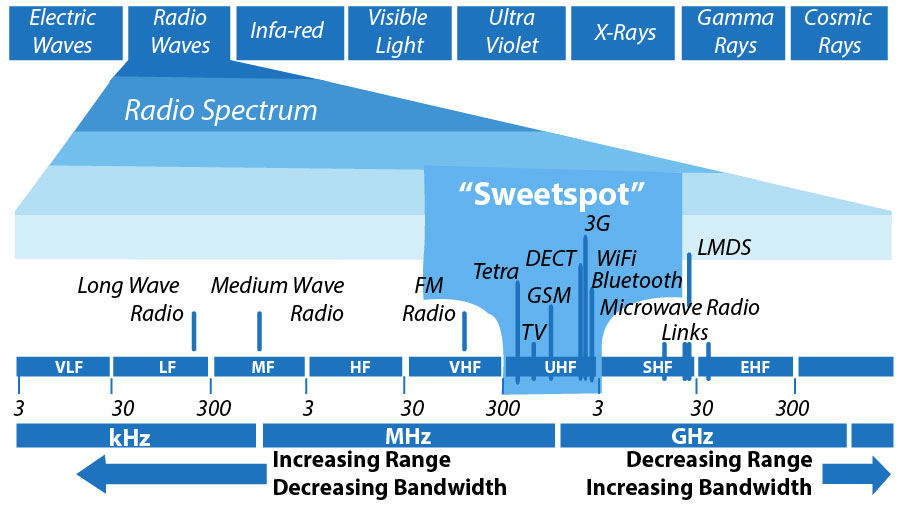
\includegraphics[width=0.95\textwidth]{./media/image1.jpeg}
		\caption{Radio spectrum's sweetspot \cite{1-34}}
	\end{Center}
\end{figure}

%%%%%%%%%%%%%%%%%%%% Figure/Image No: 1 Ends here %%%%%%%%%%%%%%%%%%%%

With the aim of reducing the interference between services, international organizations and policy-makers bind certain uses of the spectrum to small ranges of frequencies: This is called spectrum allocation. Terrestrial broadcasting used a significant part of the lower section of the UHF band in Spain, mainly 470 to 862 MHz (Considering that it also uses part of the Very High Frequency (VHF) band from 47 to 230 MHz, it is more than 50$\%$  of the spectrum below 1 GHz) \cite{1-02}. For many decades, this spectrum has been guaranteed for this terrestrial broadcasting service due to the availability of other bands for newer services and the problems to modify the existing spectrum allocation \cite{1-03}.\par

Due to the emergence of cable, satellite and Asymmetric Digital Subscriber Line (ADSL) TV, the ITU, among other international organizations, considered the need to deliver a larger number of programs with higher quality to make traditional TV broadcasting remain competitive against these newer technologies. This led to the switch from analogue TV broadcasting to digital terrestrial television \cite{1-03}.\par

Digital Terrestrial Television is based on the standard DVB-T (Digital Video Broadcasting-Terrestrial) that transmits audio, video and other information into an MPEG (Moving Picture Experts Group) transport stream. This new codification allows broadcasting to 6 digital channels with the same bandwidth that one analogue channel needed, implying more efficient spectrum management, and releasing a \textit{digital dividend} that can be used for additional TV channels and to extend the existing spectrum for mobile broadband.\par

\subsection*{The first digital dividend in Europe}
%\addcontentsline{toc}{subsection}{The first digital dividend in Europe}
In this regard, the upper part of the UHF band (790–862 MHz) was allocated to the mobile service in Region 1 in the ITU - World Radiocommunication Conference 2007 (WRC-07) \cite{1-04}. Based on this decision, the European Commission published in 2010 the Commission Decision 2010/267/UE \cite{1-05} in which \textit{«the 790-862 MHz band (}800 MHz band\textit{) was selected for terrestrial systems capable of providing electronic communications services in the European Union}».\par

Subsequently, in 2012, the European Parliament and the European Council published the decision 243/2012/EU in which forced the European members to get the digital dividend, at the latest, before 2015 \cite{1-06}.

%%%%%%%%%%%%%%%%%%%% Figure/Image No: 2 starts here %%%%%%%%%%%%%%%%%%%%

\begin{figure}[H]
	\begin{Center}
		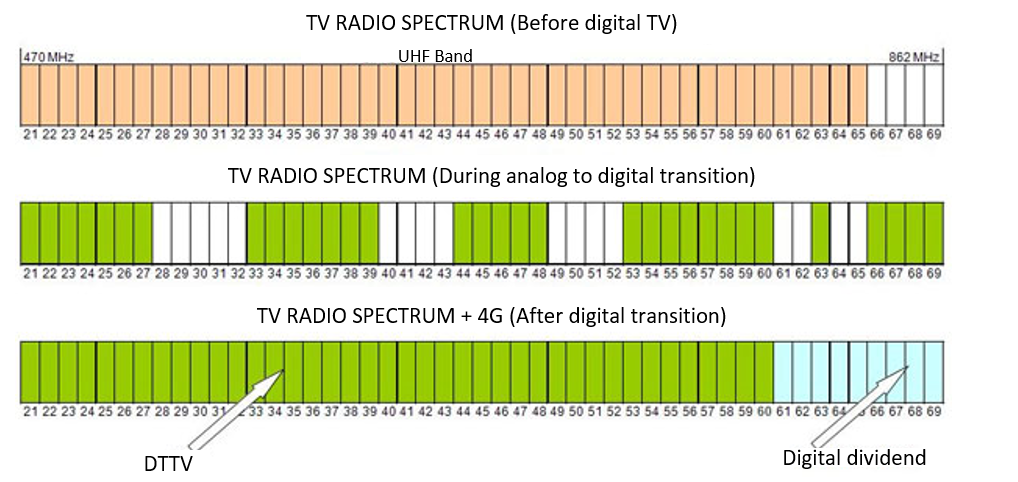
\includegraphics[width=0.95\textwidth]{./media/image2.png}
		\caption{Explanation of the Digital dividend. State Secretariat for the information society and digital agenda of Spain \cite{1-02}}
	\end{Center}
\end{figure}


%%%%%%%%%%%%%%%%%%%% Figure/Image No: 2 Ends here %%%%%%%%%%%%%%%%%%%%

Finally, the Electronic Communications Committee (ECC) within the European Conference of Postal and Telecommunications Administrations (CEPT) defined in their Report 31 \cite{1-07} their preferred harmonized frequency arrangement for the band 790-862 MHz. This arrangement would establish a downlink of 30 MHz in 6 blocks of 5 MHz each, followed by a gap of 11 MHz and an uplink of 30 MHz in 6 blocks of 5 MHz each:

%%%%%%%%%%%%%%%%%%%% Figure/Image No: 3 starts here %%%%%%%%%%%%%%%%%%%%

\begin{figure}[H]
	\begin{Center}
		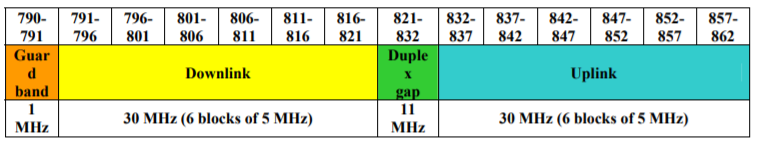
\includegraphics[width=0.95\textwidth]{./media/image3.png}
		\caption{Frequency arrangement for the 790-862 MHz band. CEPT\cite{1-07}}
	\end{Center}
\end{figure}

%%%%%%%%%%%%%%%%%%%% Figure/Image No: 3 Ends here %%%%%%%%%%%%%%%%%%%%
\subsection*{Auctions, coverage obligations, and spectrum cap}
%\addcontentsline{toc}{subsection}{Auctions, coverage obligations, and spectrum cap}
The European Member States started to develop national strategies to allocate the new spectrum (790–862 MHz) to the MNOs (Mobile Network Operators) in their countries. The terms and conditions fixed by the European Union were intended to «\textit{foster the collective use of spectrum as well as shared use of spectrum}», «\textit{enhance flexibility}» and «\textit{promote competition, investment and the efficient use of spectrum as a public good}» \cite{1-06}.\par

In this case, most governments decided to allocate spectrum through an auction procedure. The advantages of auctions are the promotion of competition and the more transparent of the spectrum since there is no subjectivity in the process. It also provides an important amount of money to governments since the competition among several bidders generally leads to higher bids. The ITU presentation in \cite{1-08} shows examples of auctions of the 800 MHz band in Europe:

%%%%%%%%%%%%%%%%%%%% Table No: 2 starts here %%%%%%%%%%%%%%%%%%%%

{
\setlength\extrarowheight{3pt}
\begin{longtable}{p{1.42in}p{1.8in}p{1.36in}}
\caption{Results of the spectrum auctions of the 800MHz band in Europe. ITU \cite{1-08}}
\endfirsthead
\multicolumn{3}{c}{\textit{continued from previous page}}\hline
\endhead\hline
\multicolumn{3}{r}{\textit{continued on next page}} \\
\endfoot
\hline 
\endlastfoot\hline
%row no:1
\multicolumn{1}{|p{1.42in}}{\Centering \textbf{Country}} & 
\multicolumn{1}{|p{1.8in}}{\Centering \textbf{Amount of auction in €}} & 
\multicolumn{1}{|p{1.36in}|}{\Centering \textbf{Year of auction}} \\
\hhline{---}
%row no:2
\multicolumn{1}{|p{1.42in}}{\Centering Austria} & 
\multicolumn{1}{|p{1.8in}}{\Centering 2,000 M€} & 
\multicolumn{1}{|p{1.36in}|}{\Centering October 2013} \\
\hhline{---}
%row no:3
\multicolumn{1}{|p{1.42in}}{\Centering Belgium} & 
\multicolumn{1}{|p{1.8in}}{\Centering 360 M€} & 
\multicolumn{1}{|p{1.36in}|}{\Centering November 2013} \\
\hhline{---}
%row no:4
\multicolumn{1}{|p{1.42in}}{\Centering Croatia} & 
\multicolumn{1}{|p{1.8in}}{\Centering 40 M€} & 
\multicolumn{1}{|p{1.36in}|}{\Centering September 2012} \\
\hhline{---}
%row no:5
\multicolumn{1}{|p{1.42in}}{\Centering Czech Republic} & 
\multicolumn{1}{|p{1.8in}}{\Centering 266 M€} & 
\multicolumn{1}{|p{1.36in}|}{\Centering November 2013} \\
\hhline{---}
%row no:6
\multicolumn{1}{|p{1.42in}}{\Centering Denmark} & 
\multicolumn{1}{|p{1.8in}}{\Centering 99 M€} & 
\multicolumn{1}{|p{1.36in}|}{\Centering 2012} \\
\hhline{---}
%row no:7
\multicolumn{1}{|p{1.42in}}{\Centering Finland} & 
\multicolumn{1}{|p{1.8in}}{\Centering 108 M€} & 
\multicolumn{1}{|p{1.36in}|}{\Centering October 2013} \\
\hhline{---}
%row no:8
\multicolumn{1}{|p{1.42in}}{\Centering France} & 
\multicolumn{1}{|p{1.8in}}{\Centering 2,600 M€} & 
\multicolumn{1}{|p{1.36in}|}{\Centering December 2011} \\
\hhline{---}
%row no:9
\multicolumn{1}{|p{1.42in}}{\Centering Germany} & 
\multicolumn{1}{|p{1.8in}}{\Centering 3,570 M€} & 
\multicolumn{1}{|p{1.36in}|}{\Centering 2010} \\
\hhline{---}
%row no:10
\multicolumn{1}{|p{1.42in}}{\Centering Ireland} & 
\multicolumn{1}{|p{1.8in}}{\Centering 854 M€} & 
\multicolumn{1}{|p{1.36in}|}{\Centering 2012} \\
\hhline{---}
%row no:11
\multicolumn{1}{|p{1.42in}}{\Centering Italy} & 
\multicolumn{1}{|p{1.8in}}{\Centering 2,960 M€} & 
\multicolumn{1}{|p{1.36in}|}{\Centering January 2013} \\
\hhline{---}
%row no:12
\multicolumn{1}{|p{1.42in}}{\Centering Lithuania} & 
\multicolumn{1}{|p{1.8in}}{\Centering 2,4 M€} & 
\multicolumn{1}{|p{1.36in}|}{\Centering October 2013} \\
\hhline{---}
%row no:13
\multicolumn{1}{|p{1.42in}}{\Centering Netherlands} & 
\multicolumn{1}{|p{1.8in}}{\Centering 3,800 M€} & 
\multicolumn{1}{|p{1.36in}|}{\Centering December 2012} \\
\hhline{---}
%row no:14
\multicolumn{1}{|p{1.42in}}{\Centering Portugal} & 
\multicolumn{1}{|p{1.8in}}{\Centering 270 M€} & 
\multicolumn{1}{|p{1.36in}|}{\Centering 2012} \\
\hhline{---}
%row no:15
\multicolumn{1}{|p{1.42in}}{\Centering Romania} & 
\multicolumn{1}{|p{1.8in}}{\Centering 682 M€} & 
\multicolumn{1}{|p{1.36in}|}{\Centering September 2012} \\
\hhline{---}
%row no:16
\multicolumn{1}{|p{1.42in}}{\Centering Spain} & 
\multicolumn{1}{|p{1.8in}}{\Centering 1,300 M€} & 
\multicolumn{1}{|p{1.36in}|}{\Centering July 2015} \\
\hhline{---}
%row no:17
\multicolumn{1}{|p{1.42in}}{\Centering Sweden} & 
\multicolumn{1}{|p{1.8in}}{\Centering 233 M€} & 
\multicolumn{1}{|p{1.36in}|}{\Centering 2009} \\
\hhline{---}
%row no:18
\multicolumn{1}{|p{1.42in}}{\Centering Switzerland} & 
\multicolumn{1}{|p{1.8in}}{\Centering CHF 996 Million} & 
\multicolumn{1}{|p{1.36in}|}{\Centering July 2005} \\
\hhline{---}
%row no:19
\multicolumn{1}{|p{1.42in}}{\Centering The UK} & 
\multicolumn{1}{|p{1.8in}}{\Centering 2,700 M€} & 
\multicolumn{1}{|p{1.36in}|}{\Centering February 2013} \\
\hhline{---}


\end{longtable}}
%%%%%%%%%%%%%%%%%%%% Table No: 2 ends here %%%%%%%%%%%%%%%%%%%%

For a deeper study of the benefits of the different kinds of auctions, the reader is referred to \cite{1-09}.\par

Due to the favourable propagation properties of the 800 MHz band, the European Union Multiannual Radio Spectrum Policy [1-06] article 3c) state that the Member States should «\textit{foster access to broadband at a speed of not less than 30 Mbps by 2020 for all Union citizens}»\textit{. }This decision is focused on homogenizing the end-user speed of the mobile network, so that the difference between the urban areas, with higher speeds, and rural areas, with lower speeds, can be reduced. \par

Even though each country implemented different variations of this policy, most of the biggest countries in Europe imposed some coverage and rollout obligations for those MNOs that sought access to blocks at 800 MHz. For example, the Spanish government obliged MNOs to elaborate a report on how they will jointly meet this requirement \cite{1-10} and the office of communications of UK (Ofcom) set a 95$\%$  population coverage with at least 2 Mbps in each of the UK nations in one of the blocks \cite{1-11}. These coverage obligations will be examined in greater detail in the following chapters.\par

Spectrum integration is the last characteristic of the spectrum auction in Europe. Most governments imposed a certain cap to ensure that this natural resource is distributed among the principal MNOs. In most countries, it was set as a limit on the amount of spectrum that each operator could hoard across all the bands, as a cap in a specific band or as a combination of both. In the following chapters, this spectrum cap will be examined for all the countries under study. This paper of the Global System for Mobile Communications (GSMA) \cite{1-11} covers the historical evolution of the spectrum cap worldwide.\par

\section{5G}
%\addcontentsline{toc}{subsection}{5G}
Initially, mobile networks were mainly intended for voice. As technology evolved, users began to use mobile phones for more purposes: web browsing was standardized in 3G, and 4G allowed users to consume higher-speed data and video streaming, among other examples. This increasing trend is expected to be even more pronounced now, given the emergence of technologies such as 4K video streaming and virtual and augmented reality, that will require higher bandwidth and capacity \cite{1-14}. Moreover, according to the VNI (Visual Networking Index) of Cisco \cite{1-15}, mobile data traffic will increase sevenfold between 2016 and 2021 and Video-on-Demand (VoD) traffic will nearly double by 2021.\par

Apart from the natural growth of the data traffic demand, the industry is aiming to develop new communication technologies with extremely low latency, ultra-reliable communications with low latencies or that could allow for a higher density of devices connected to the network. These features will enable the development of new possibilities such as smart cities, cooperative automated driving, and, as well as to enable the full potential of the Internet of Things \cite{1-16}.\par

Therefore, the following three main potential use cases \cite{1-17} upon technical requirements have been defined:\par

\begin{itemize}
	\item Use case 1: Enhanced mobile broadband\par

This scenario focuses on providing very high data rates for future mobile broadband users to experience instantaneous connectivity without delays. Data rates considered are at least 1 Gb/s or more to support ultrahigh-definition video, virtual reality applications and even more speed to support mobile cloud services. \par

	\item Use case 2: Massive machine-type communications\par

This scenario focuses on the efficient handling of a very large number of devices (including, e.g., machine type devices and sensors) with widely varying requirements. Current mobile network systems capacity should expand to support several billions of applications and hundreds of billions of machines connected simultaneously. \cite{1-18} This will enable a faster development of Smart Cities, Smart Logistics, and Intelligent Agriculture.\par

	\item Use case 3: Ultra-reliable and low latency communications\par

This scenario focuses on new applications and use cases with very strict requirements on latency and reliability. Networks with less than one-millisecond latency would enable to support real-time mobile control, vehicle-to-vehicle applications and communications and robotic-assisted surgery among others.\par

5th generation mobile networks are the proposed next communication standards that will allow all these industry developments to take place. This triangle is commonly used to show all the scenarios in which the 5G is intended to be the real technology standard of the near future:

%%%%%%%%%%%%%%%%%%%% Figure/Image No: 4 starts here %%%%%%%%%%%%%%%%%%%%

\begin{figure}[H]
	\begin{Center}
		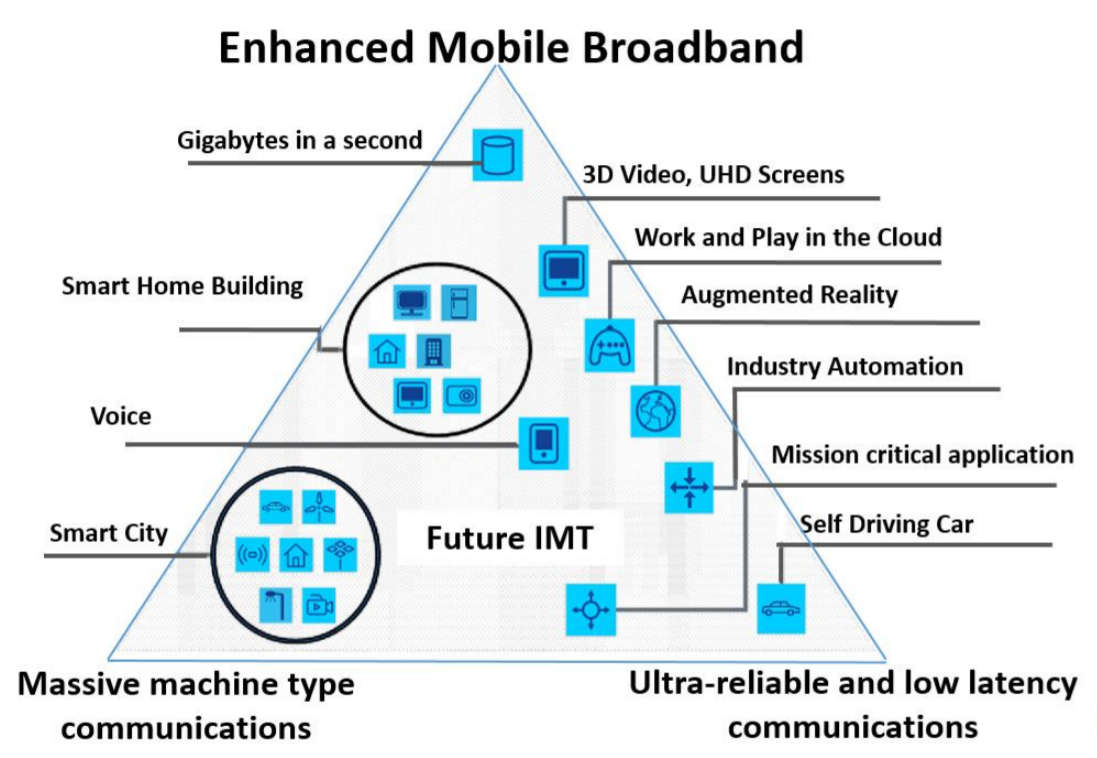
\includegraphics[width=0.95\textwidth]{./media/image4.png}
		\caption{Potential use cases of the 5G networks. ITU-T workshops April 2017\cite{1-17}}
	\end{Center}
\end{figure}


%%%%%%%%%%%%%%%%%%%% Figure/Image No: 4 Ends here %%%%%%%%%%%%%%%%%%%%

\end{itemize}
\section{Radio Spectrum for 5G}
%\addcontentsline{toc}{subsection}{Radio Spectrum for 5G}
Although the mobile industry, academic institutions, and international standard-making bodies are developing technologies that will be central to 5G, the success of the service rollout will also be heavily reliant on policy-makers. 5G services will be heavily dependent on governments and regulators supporting timely access to sufficient spectrum resources and under the right conditions. In this paper \cite{1-19} from November 2016, GSMA set three key frequency ranges to deliver widespread coverage and support all use cases. The three ranges are Sub-1 GHz, 1-6 GHz and above 6 GHz. Also, in an ITU event for Europe in 2017 \cite{1-20}, Nokia showed this diagram with the pioneer bands that Europe will use for 5G. These frequencies with differing characteristics will enable to cover all the scenarios described above.



%%%%%%%%%%%%%%%%%%%% Figure/Image No: 5 starts here %%%%%%%%%%%%%%%%%%%%

\begin{figure}[H]
	\begin{Center}
		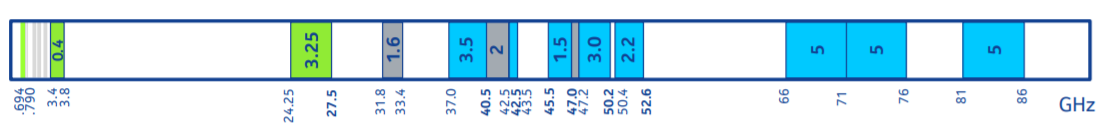
\includegraphics[width=0.95\textwidth]{./media/image5.png}
		\caption{Possible future 5G bands. Nokia\cite{1-20}}
	\end{Center}
\end{figure}


%%%%%%%%%%%%%%%%%%%% Figure/Image No: 5 Ends here %%%%%%%%%%%%%%%%%%%%

\subsection*{Sub1 GHz}
%\addcontentsline{toc}{subsubsection}{Sub1 GHz}
Lower frequencies propagate further in the environment, and therefore it is possible to cover more area per antenna. Therefore, sub-1 GHz spectrum is needed to extend high speed 5G mobile broadband coverage across suburban and rural areas and for new services like connected cars and smart sensors.\par

In fact, there is some mobile spectrum in this range that will be used in the near future. The European Commission has already decided that 700 MHz will be used to support 5G services in Europe \cite{1-21}. Similarly, the Federal Communications Commission of the United States (FCC) has indicated that the 600 MHz band could be used to drive 5G services in the United States.\par

\subsection*{1 - 6 GHz}
%\addcontentsline{toc}{subsubsection}{1 - 6 GHz}
The spectrum from 1-6 GHz offers a mixture of coverage and capacity for 5G services. That is why there is a reasonable amount of existing mobile broadband spectrum identified within this range that could potentially be allocated to 5G technologies. \par

Using spectrum within the 3.3 and 3.8 GHz range is highly interesting for initial commercial 5G services. For example, Ofcom, the UK regulator, published in April the results of the spectrum auction for the band of 2.3 and 3,4 GHz \cite{1-22}. Other mobile bands in the 1-6 GHz range that are currently used for 3G and 4G services should be gradually refarmed for 5G. In this regard, the RSPG stated in November 2016 \cite{1-23} that 3.6 GHz (3400-3800 MHz) will be the first primary band for 5G and bring the necessary capacity for new 5G services.\par

Ofcom launched in April 2016 a Call for Inputs \cite{1-24} asking for opinions on the potential of the 3.8 to 4.2 GHz band for 5G development. However, after that consultation, Ofcom decided not to consider this band as a current priority \cite{1-25} candidate for mobile services in the UK– which is the top priority level in Ofcom strategies – but kept it in the second level: «high priority» \cite{1-26}. \par

\subsection*{Above 6 GHz}
%\addcontentsline{toc}{subsubsection}{Above 6 GHz}
Part of the usage of the networks will occur within crowded cities where networks will have to be designed for capacity rather than for coverage, so the benefits of lower frequencies will be insignificant (The main benefit is that they do propagate further than higher ones) and the differences between low and high frequencies become much less significant.\par

Higher frequencies are cheaper and not so prone to have coverage obligations as the lower ones since they are not so useful for broadcasting in long distances and no MNOs would pay for them. They also have large gaps that could be allocated for mobile broadband services quite fast, giving a significant extra bandwidth to the network. These wide bandwidths will be the key for the fastest 5G services, this part of the spectrum is intended for the ultrahigh speed mobile broadband scenario. \par

The spectrum targeted above 6 GHz is expected to comprise a mixture of licensed and unlicensed mobile bands. 5G mobile bands should be agreed at WRC-19, under Agenda Item 1.13, \cite{1-27} which is considering the following bands for 5G: 24.25-27.5 GHz, 31.8-33.4 GHz, 37-43.5 GHz, 45.5-50.2 GHz, 50.4-52.6 GHz, 66-76 GHz and 81-86 GHz. However, some countries are also investigating other mobile bands above 6 GHz for 5G services, which will not be considered at WRC-19.\par

In November 2016, the Radio Spectrum Policy Group (RSPG) of the European Commission pointed out that the pioneer band in this range will be 26 GHz (24.25-27.5 GHz) \cite{1-23}, which they describe as the band that will «\textit{provide ultra-high capacity for innovative new services, enabling new business models and sectors of the economy to benefit from 5G}».\par

\subsection*{The importance of the 700 MHz band}
%\addcontentsline{toc}{subsubsection}{The importance of the 700 MHz band}
The 700 MHz band will have a key role in this paper due to a combination of two factors. As it has been introduced in previous chapters, once it is reallocated, it will be the band with the best propagation properties available for mobile communications in Europe. Now that all urban areas benefit from high-speed mobile connections, the European Union is giving top priority to the development of high-speed access in suburban and rural areas \cite{1-28}. Apart from that, the fact that the second digital dividend is a reality in most countries of Europe, it will enable a faster roll-out of the 5G of mobile communications, which is expected by 2020 \cite{1-29}. \par

\section{State of the Art}
%\addcontentsline{toc}{subsection}{State of the Art}
The aim of this Master Thesis is to analyze how the actions of the regulatory bodies will affect in different ways the rollout of 5G in Europe. Hence, this chapter explores the literature related to the measures that countries have taken to foster a nationwide high-speed mobile communications access previously, with particular emphasis on mobile coverage obligations. \par

\subsection*{The weight of the spectrum’s price factors}
%\addcontentsline{toc}{subsubsection}{The weight of the spectrum’s price factors}
Insua et. al explores in \cite{1-30} the parameters that determine the price that mobile operators pay for radio spectrum in some European countries and applies multiple regression analysis to generate a model that, based on parameter combinations, predicts the outcome of spectrum auctions when they have not taken place yet.\par

In this paper, Insua et al state that the main factors that affect the price of the spectrum are the frequency band and the country in which the auction is taking place, while other factors such as the number of competitors or the year in which this bidding takes place have a minor impact. The following table shows the adjusted R as a measurement of the relation between the variable and the price of the spectrum:


%%%%%%%%%%%%%%%%%%%% Figure/Image No: 6 starts here %%%%%%%%%%%%%%%%%%%%

\begin{figure}[H]
	\begin{Center}
		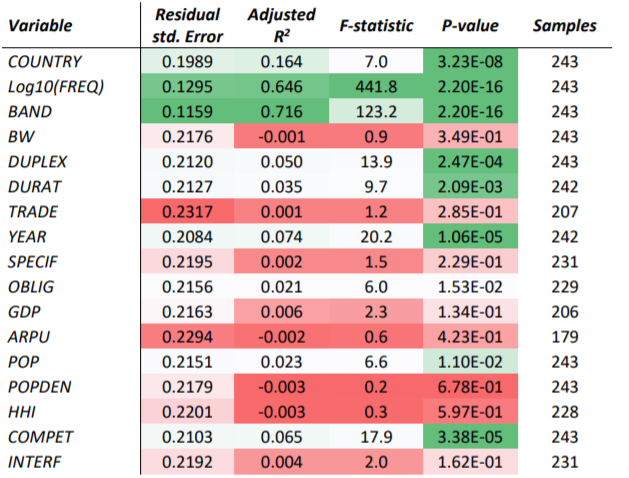
\includegraphics[width=0.95\textwidth]{./media/image6.png}
		\caption{Factors of the bids amounts in spectrum auctions. Insua et. al\cite{1-30}}
	\end{Center}
\end{figure}


%%%%%%%%%%%%%%%%%%%% Figure/Image No: 6 Ends here %%%%%%%%%%%%%%%%%%%%

\subsection*{The usage of spectrum aggregation limits}
%\addcontentsline{toc}{subsubsection}{The usage of spectrum aggregation limits}
The work by Cave $\&$  Webb \cite{1-31} for the FCC (Federal Communications Commission) of the United States analyzes the spectrum caps imposed by the European regulators. Despite the reluctance in the United States to use spectrum-aggregation limits based on the belief that it would reduce the price of the spectrum, the study states that almost all European regulators established one.\par

According to the paper, European regulators looked for a balance between raising revenues and fostering competition by setting a spectrum cap that limits the amount of spectrum for which one MNO can bid. The study reveals that there was \textit{«no difference between auctions where limits were hit and the case where the limit was not»} and they also state that «\textit{there is no evidence that [spectrum caps] do materially reduce revenue».}\par

\subsection*{Ofcom: Connected Nations 2017}
%\addcontentsline{toc}{subsubsection}{Ofcom: Connected Nations 2017}
This Ofcom´s annual report, published in December 2017, analyzes the evolution of the coverage of broadband and mobile networks of the UK in 2017 \cite{1-32}. They define that an area has data services coverage when «\textit{Nearly all connections [95$\%$  of the time] should deliver a speed of at least 2Mbit/s. This is fast enough to allow users to browse the Internet and watch the glitch-free mobile video».}\par

This report states that the indoor coverage at home or at the office is of 85$\%$  for mobile data services,\ while outdoor is of just 63$\%$ .  Ofcom has also a category for coverage in roads in which they set it to 58$\%$ . This category considers the reduction of mobile signal levels as they travel through the metal frame of the vehicle and is a key measure due to the increased interest in connected cars which will be possible thanks to the 5G technologies.\par

Ofcom also compares the coverage per nation in the UK and warns about the difference in coverage between urban and rural areas and between England and other nations. Northern Ireland has a greater proportion of dispersed properties throughout the countryside, making it more difficult to deliver a proper indoor coverage. In fact, it is the only nation that has a better outdoor data services coverage than indoor. On the other side, in Scotland, with low population densities and large and often mountainous areas, geographic outdoor coverage is so low, while the indoor coverage is reasonably good. \par

Based on these results and the strategical aspect of the data mobile services, Ofcom states the necessity of setting coverage obligations to minimize the difference between nations and regions of the UK.



%%%%%%%%%%%%%%%%%%%% Figure/Image No: 7 starts here %%%%%%%%%%%%%%%%%%%%

\begin{figure}[H]
	\begin{Center}
		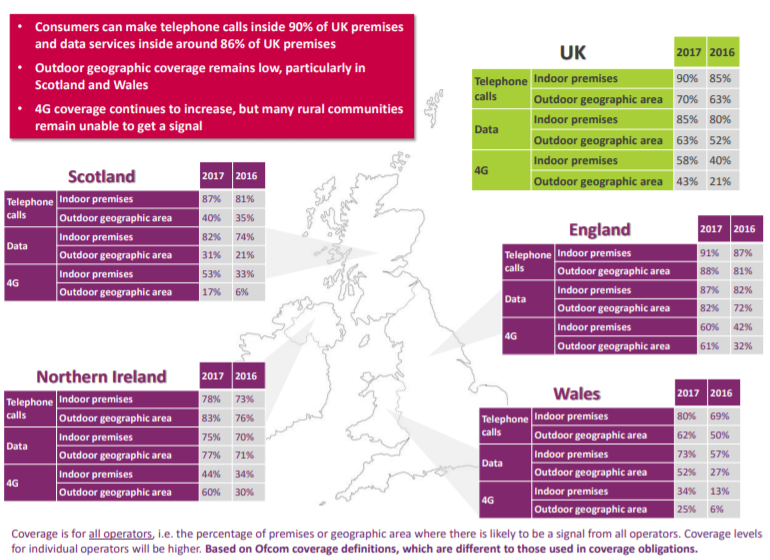
\includegraphics[width=0.95\textwidth]{./media/image7.png}
		\caption{Ofcom analysis of operator coverage, June 2017\cite{1-32}}
	\end{Center}
\end{figure}


%%%%%%%%%%%%%%%%%%%% Figure/Image No: 7 Ends here %%%%%%%%%%%%%%%%%%%%

\subsection*{Technical analysis of the cost of extending an 800 MHz mobile broadband coverage obligation for the UK}
%\addcontentsline{toc}{subsubsection}{Technical analysis of the cost of extending an 800 MHz mobile broadband coverage obligation for the UK}
This document produced by Real Wireless on behalf of Ofcom \cite{1-33} examines the investment effort that MNOs must carry out in the UK to comply with the coverage obligations imposed by Ofcom to the operator that won the spectrum block with coverage obligations in the 800 MHz auction in 2013. This analysis provides some important insights for this Master Thesis:\par

\begin{itemize}
	\item According to this analysis, upgrading existing sites in the UK to use a block of 5 MHz 800 MHz would be as low as 61$\%$  of indoor coverage obligation.\par

	\item Rising the transmit power will not imply a significant coverage gain since gains are limited due to terrain and uplink limitations.\par

	\item Costs of achieving a specific indoor coverage are approximately 20$\%$  lower using 2 blocks of 10 MHz that using 2 blocks of 5 MHz in the 800 MHz band.\par

	\item The marginal cost of rising the indoor coverage from 95$\%$  to 98$\%$  is greater than the required to increase the coverage from 90$\%$  to 95$\%$ .
\end{itemize}\par


\chapter{On the problem to set coverage obligations}
%\addcontentsline{toc}{section}{On the problem to set coverage obligations}
This chapter undertakes a detailed analysis of the problem to set coverage obligations. The first part analyses the most frequently used spectrum allocation mechanisms and the reasons why coverage obligations are normally used to force MNOs to provide a minimum broadband access speed. After that, I analyze all the parameters that define a coverage obligation set (Time frame, the scope, if it is only for data service or for data and voice service, etc.). Finally, I review the coverage obligations set for 800 MHz for Spain, the UK, Germany, and France to illustrate how these were set in one of the latest spectrum auctions.\par

\section{Mechanisms to allocate spectrum}
%\addcontentsline{toc}{subsection}{Mechanisms to allocate spectrum}
According to this document of the Spanish Ministry for the Digital Agenda (MINETAD) \cite{2-01}, there were several mechanisms to assign public spectrum to mobile operators in the past, namely:\par

\begin{itemize}
	\item Administrative grant: This allocation had no transparency nor quickness because it was the responsibility of the government to decide the frequency band, technology and other specifications of the service \cite{2-02}. In the UK, licenses were awarded for a specific technology and use and without raising interests until the 1998 Wireless Telegraphy Act \cite{2-06}]. This act enabled the usage of auctions to grant licenses and the first auction was in 2000 for 3G mobile licenses.\par

	\item Lottery: The spectrum is partitioned and given to the MNOs. This mechanism is transparent and quicker, although it is neither fair nor efficient because the allocation is not related to any technical factor. This mechanism was used in the distribution of the 3G spectrum in the U.S.\par

	\item Scoring rule: Using scoring rules, the government notify the set of factors that will weigh in the decision and the MNOs that are interested in the spectrum just send their applications. The decision is taken by the government, which can incur in lack of transparency.\par

	\item Auctions: This is a transparent and raising-oriented mechanism that became more popular since 2000 and 2001 when countries that created auctions to allocate the spectrum for 3G raised pretty much money than countries that used the traditional public competition.
\end{itemize}\par

Once spectrum is allocated, regulatory bodies must ensure that it is used in an effective and fair way, enforcing MNOs to invest nationwide and not only in the most cost-effective areas. Hence, policies should target primarily the least populated areas, where the cost of user capacity is higher. According to this GSMA report \cite{2-03}, there are three types of areas depending on their economic viability with regards to new mobile broadband rollout:\par

\begin{itemize}
	\item Type 1: Areas which will be covered by network competition.\par

	\item Type 2: Areas which can only be covered with network-sharing or a single network.\par

	\item Type 3: Areas which can only be covered with some form of public funding.
\end{itemize}\par

Regulators must focus their efforts on fostering the deployment of mobile broadband networks in areas of type 2 and 3. In the paper, GSMA also defines three main mechanisms regulators can make use of:\par

\begin{itemize}
	\item Tool 1: Promoting voluntary infrastructure sharing in rural areas.\par

	\item Tool 2: Licensing of low-frequency spectrum in combination with coverage obligations.\par

	\item Tool 3: Using public finances to (co)fund rollout in uneconomic rural areas.
\end{itemize}\par

Infrastructure sharing is a tool that is widely used in Europe due to the difference in the size of the companies in the telecom sector. Examples were the national roaming agreement in Spain between Yoigo and Vodafone since Yoigo’s coverage was limited to urban areas and the agreement between H3G and O2 in the UK. These GSMA report \cite{2-04} has a complete list of agreements in European countries.\par

According to the Florence School of Regulation [5], the third tool is not advised as they suggest that \textit{«simply reducing the immediate and direct cost of access to broadband connections through supply-side policies may not be enough to stimulate broadband subscriptions»}, since the perceived benefits from broadband access do not compensate the cost of the broadband connection for end-users. This tool seems to be interesting for the MNOs because they could reduce the CAPEX, but end users would not choose to pay for a broadband service that they would not use and, therefore, MNOs would not deploy new assets. \par

Therefore, only the second tool can help to truly stimulate mobile coverage in rural areas, due to the rollout of more mobile coverage is not subsidized but mandatory. This course of action will probably also foster end-users from rural areas to use mobile services.\par

The following figure, obtained from \cite{2-03}, shows the effect that adding coverage obligations have on the price of the spectrum. It can be considered as a priced reduction in exchange for promoting an obligatory inversion in new coverage for several years (until the threshold coverage is reached).

%%%%%%%%%%%%%%%%%%%% Figure/Image No: 8 starts here %%%%%%%%%%%%%%%%%%%%

\begin{figure}[H]
	\begin{Center}
		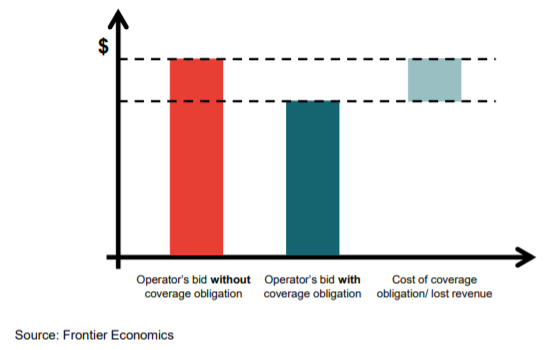
\includegraphics[width=0.95\textwidth]{./media/image8.png}
		\caption{Impact of the coverage obligations in the operator's bid \cite{2-03}}
	\end{Center}
\end{figure}


%%%%%%%%%%%%%%%%%%%% Figure/Image No: 8 Ends here %%%%%%%%%%%%%%%%%%%%
As an example, the UK spectrum allocation history is accurately explained in this publication of the parliament of the UK \cite{2-07}. Spain defined different coverage obligations for each spectrum band that has been allocated for mobile communications:\par
\begin{itemize}
	\item 800 MHz: 30 Mbit/s available to 90 $\%$  of citizens living in population centres of less than 5.000 inhabitants.\par

	\item 900 MHz: Population entities of less than 1000 inhabitants with a minimum level of -90dBm of UMTS 900 outdoor.\par

	\item 1800 MHz: Coverage obligation in cities higher than 500,000 inhabitants before 1999.\par

	\item 2100 MHz: Coverage obligation in cities higher than 250,000 inhabitants before 2003.\par

	\item 2600 MHz: No coverage obligations.
\end{itemize}\par

In March 2015, the ECC CEPT elaborated a big report about mobile coverage obligations \cite{2-08 which contains several classifications of the coverage obligations and answers that policymakers of 29 countries gave to a set of questions about their coverage obligations.  This report shows how widespread is the usage of coverage obligations at this time. According to the 29 countries in the survey:\par

\begin{itemize}
	\item 24 administrations have imposed coverage obligations regarding the voice service in one or more frequency bands;\par

	\item 25 administrations have imposed coverage obligations regarding the data service in one or more frequency bands.
\end{itemize}\par











\section{Defining coverage obligations}
%\addcontentsline{toc}{subsection}{Defining coverage obligations}
According to \cite{2-08} and \cite{2-03}, coverage obligations can be defined in multiple ways regarding several factors. All the examples in this section are answers that the countries submitted to the ECC CEPT questionnaire:\par

\begin{itemize}
	\item The object of study:\par

\begin{itemize}
	\item Population coverage: The operator needs to cover a percentage of the population.\par

	\item Area coverage: The operator needs to cover a percentage of the territory.\par

\end{itemize}
\end{itemize}
\begin{itemize}
	\item Timeframe:\par

\begin{itemize}
	\item Fixed in time: Certain percentage covered in certain years.\par

	\item Gradual through time: The percentage to cover grows every certain year.\par
\end{itemize}
\end{itemize}
For example, France «\textit{Gradual through time»} example will be studied in the following chapter and Belgium defined these three milestones: 30$\%$  of population 2 years after obtaining a license, 70$\%$  of population 4 years after obtaining a license and 98$\%$  of population 6 years after obtaining a license. In the opposite case, Spain and the UK defined just one milestone in 2020 and 2017 respectively.\par

\begin{itemize}
	\item Frequency band:\par

\begin{itemize}
	\item Using a specific band.\par

	\item Using any band allocated to the operator.\par

\end{itemize}
\end{itemize}
As an example, operators in Spain and Portugal can fulfil the data coverage obligations using any frequency band or technology allocated for mobile operators. On the contrary, each band has its own coverage obligation in France.\par


\begin{itemize}
	\item Spectrum’s blocks differentiation:\par

\begin{itemize}
	\item All blocks of the band have the same coverage obligations.\par

	\item Some blocks have more coverage obligations than others.\par
\end{itemize}
\end{itemize}
In Finland, there are two different coverage obligation sets in the 800 MHz frequency band, one has higher obligations compared to two other licenses: One mobile network has to cover 95 $\%$  of the population of mainland Finland within three years of the license period, and 99 $\%$  of the mainland of Finland's population within five years of the license period; two other mobile networks have to cover 97 $\%$  of the population of mainland Finland within five years of the license period begins.  Another example is the UK, where Ofcom offered one block of spectrum bigger than the others, but with data service coverage obligations. We will study this case later in this chapter \cite{2-09}.\par

\begin{itemize}
	\item The scope of the coverage obligation:\par

\begin{itemize}
	\item Each operator must fulfil the coverage obligation on their own.\par

	\item Coverage obligations are designed to be covered collaboratively.\par
\end{itemize}
\end{itemize}
When each spectrum’s block has different coverage obligations, they are usually enforced separately to each operator. This makes sense since if the distribution of the spectrum is not equal among all the operators, obligations must vary. However, the Spanish government allowed fulfilling the data coverage obligation rate using a combination of resources of all the available operators. The following chapter explains it extensively.\par

\begin{itemize}
	\item Area-specific obligations:\par

\begin{itemize}
	\item The coverage obligations affect all the territory equally.\par

	\item The country can be divided and coverage obligations are defined independently for each slice or only some areas are under specific coverage obligations.
\end{itemize}
\end{itemize}

Two examples will be explained later: the UK and the coverage obligation per nation and France and their $``$Area of high priority$"$ .\par

Once coverage obligations are defined, two more points have to be defined: the parameters that the policymaker will evaluate to check if the MNO has fulfilled the coverage obligations and which are the mechanisms that the policymakers will use to evaluate those parameters.\par

\subsection*{How to evaluate if the data coverage obligation is fulfilled:}
%\addcontentsline{toc}{subsubsection}{How to evaluate if the data coverage obligation is fulfilled:}
The questionnaire of ECC CEPT \cite{2-08} had also one question about the kind of criteria that defined that coverage obligations are fulfilled or not. Answers of the countries showed the following criteria:\par

\begin{itemize}
	\item Maximum theoretical data rate.\par

	\item Downlink data rate.\par

	\item Minimum of the population to be covered with a specific minimum data rate.\par

	\item Specific outdoor or indoor coverage.\par

	\item Limit values for RSRP (Reference Signal Received Power) and SINR (Signal-to-Interference-plus-Noise Ratio).
\end{itemize}\par

\subsection*{How to enforce telecom operators to meet coverage obligations}
%\addcontentsline{toc}{subsubsection}{How policymaker enforce telecom operators to meet coverage obligations}
There is no international plan, not even a European plan, to standardize the control of the growth of the coverage in the country. According to the questionnaire cited above, countries use three main strategies to control the coverage:\par

\begin{itemize}
	\item Regulators can use the information provided by the operators to verify the progress of the investments to increase the coverage in the country.\par

	\item If operators do not publish this information, regulators can use other information of the operators, such as the location of the base stations, antennas’ propagation model, network load, etc., to estimate the coverage theoretically.\par

	\item Finally, regulators can complement this information with some field measurements that validate the information supplied, but this is an expensive measure. It can be useful for some key areas and to validate the estimations made with the other strategies.
\end{itemize}\par















\section{Coverage obligations in the first digital dividend}
%\addcontentsline{toc}{subsection}{Coverage obligations in the first digital dividend}
The terms and conditions that telecom operators must follow to have access to the 800 MHz band depend on the country, but most of the European regulators included coverage obligations in the auctions. As everything suggests that the coverage obligations of the second dividend will be like the ones applied years ago, the first digital dividend will be analyzed.\par

\subsection*{Spain}
\addcontentsline{toc}{subsection}{Spain}
The Sustainable Economy Act of March 4, 2011 (Act 2/2011) \cite{2-10} established in the Article 51 that the 800MHz band was meant for advanced services for electronic communications and that it should be free to allocate before January 1, 2015. Regardless of what was said, it did not happen until April 1, 2015, because the Spanish Supreme Court declared that the channels of one TV multiplex where assigned without public competition \cite{2-12}.\par

MINETUR (The Industry, Tourism and Commerce ministry) decided that each of the spectrum blocks of the auction should have 5 MHz for uplink and downlink. Therefore, there were 6 blocks for each direction. According to this ministry \cite{2-11}, Vodafone, Orange – as France Telecom – and Telefónica got each of them, 2 blocks for uplink and 2 for downlink, dividing the spectrum equally between them. The block which was supposed to have more noise from the Terrestrial TV signals was assigned to Orange in exchange for paying less for it.


%%%%%%%%%%%%%%%%%%%% Figure/Image No: 9 starts here %%%%%%%%%%%%%%%%%%%%

\begin{figure}[H]
	\begin{Center}
		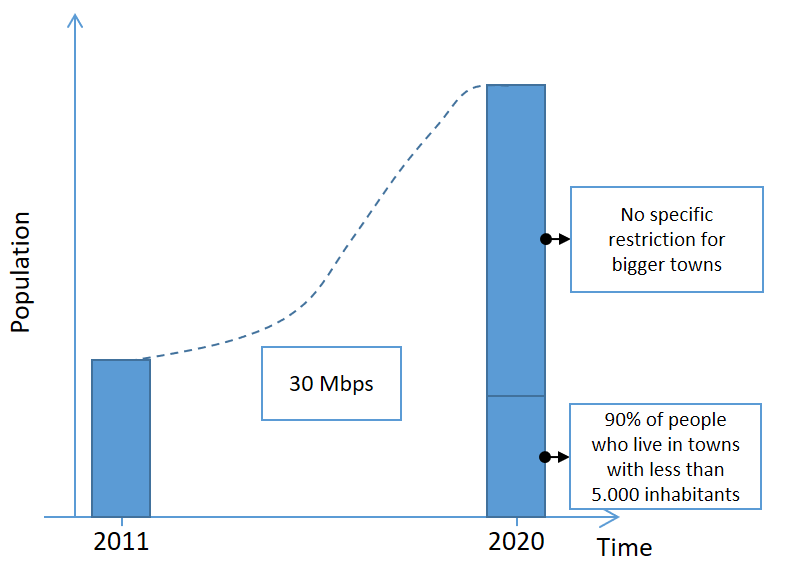
\includegraphics[width=0.95\textwidth]{./media/image9.png}
		\caption{Coverage obligations in Spain. Source: Author}
	\end{Center}
\end{figure}


%%%%%%%%%%%%%%%%%%%% Figure/Image No: 9 Ends here %%%%%%%%%%%%%%%%%%%%

According to what it is established in the article 6.2 of the Royal Decree 458/2011 (Spanish Official State Gazette of April 29, 2011), MINETUR established that those MNOs that have spectrum in the 800 MHz band have to create a joined plan to offer at least 30 Mbps to 90$\%$  of the inhabitants of population sizes smaller than 5,000 people before January 1, 2020.\par




\subsection*{The United Kingdom}
\addcontentsline{toc}{subsection}{The United Kingdom}
The policymaker responsible for defining the guidelines of the digital dividend in the United Kingdom was Ofcom. This public agency published on March 22, 2011, a consultation \cite{2-13} with the key conditions to request the MNOs. This consultation was about how Ofcom should award this new spectrum in a way that secures the best use for the benefit of citizens and consumers. In this consultation, the policymaker defined a spectrum auction with limits in the spectrum that each MNO can win:\par
\begin{itemize}
	\item Lower limits, defined as floors, are the minimum spectrum that an operator needs to be considered as a $``$credible national wholesaler$"$  in this situation. The auction would be valid if four or more operators end with at least one of the following options:\par

\begin{itemize}
	\item 2x5 MHz of sub-1 GHz and 2x20 MHz of 2.6 GHz; or
	\item 2x5 MHz of sub-1 GHz and 2x15 MHz of 1800 MHz; or
	\item 2x10 MHz of sub-1 GHz and 2x15 MHz of 2.6 GHz; or
	\item 2x10 MHz of sub-1 GHz and 2x10 MHz of 1800 MHz; or
	\item 2x15 MHz of sub-1 GHz.\par
\end{itemize}
	\item Upper limits, defined as caps, are the maximum amount of spectrum each participant could win in the auction. The caps were: 2x27.5 MHz of sub-1 GHz spectrum and 2x105 MHz of mobile spectrum in total.\par
\end{itemize}

Ofcom divided the available spectrum into blocks of 5 MHz, paired and with reverse duplex direction. This is illustrated in the figure below:



%%%%%%%%%%%%%%%%%%%% Figure/Image No: 10 starts here %%%%%%%%%%%%%%%%%%%%

\begin{figure}[H]
	\begin{Center}
		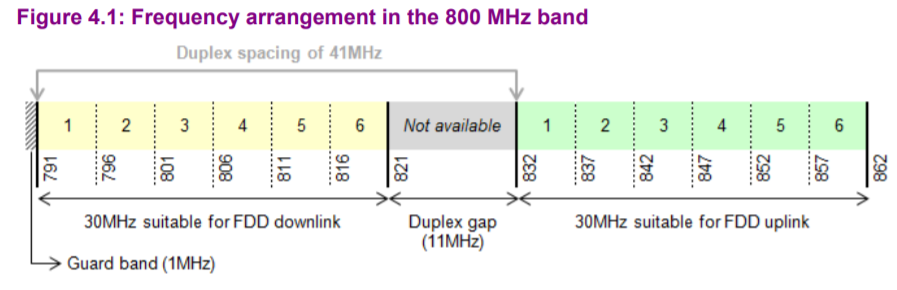
\includegraphics[width=1.00\textwidth]{./media/image10.png}
		\caption{Frequency arrangement in the UK in the 800 MHz band. Ofcom\cite{2-13}}
	\end{Center}
\end{figure}


%%%%%%%%%%%%%%%%%%%% Figure/Image No: 10 Ends here %%%%%%%%%%%%%%%%%%%%

Moreover, Ofcom required two types of coverage obligations:\par

First, a coverage obligation in only one license \textit{«for the 800 MHz spectrum to deploy a network capable of providing mobile telecommunication services with a sustained downlink speed of 2Mbps with a 90$\%$  probability of indoor reception to an area within which at least 95$\%$  of the UK population lives by the end of 2017»} and\textit{ «to provide a minimum level of indoor data coverage to 98$\%$  of all UK premises by 31 December 2017»}.



%%%%%%%%%%%%%%%%%%%% Figure/Image No: 11 starts here %%%%%%%%%%%%%%%%%%%%

\begin{figure}[H]
	\begin{Center}
		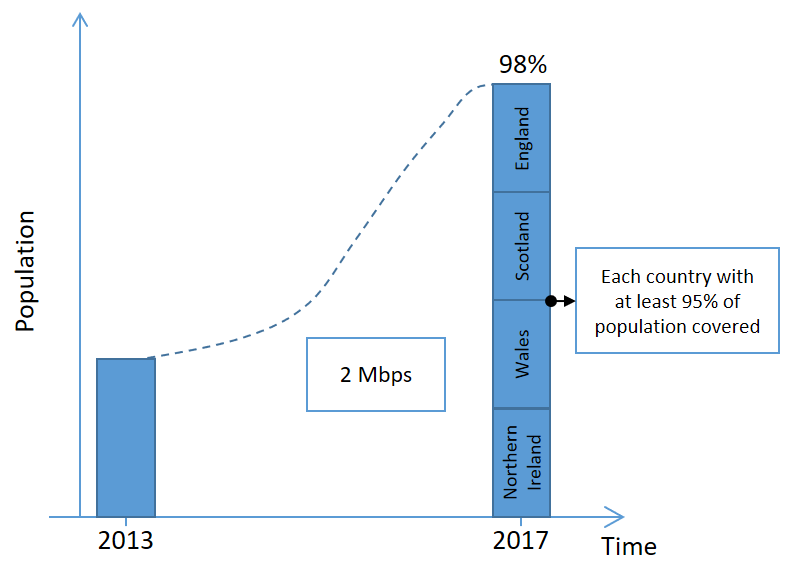
\includegraphics[width=0.80\textwidth]{./media/image11.png}
		\caption{Coverage obligations in the UK. Source: Author}
	\end{Center}
\end{figure}


%%%%%%%%%%%%%%%%%%%% Figure/Image No: 11 Ends here %%%%%%%%%%%%%%%%%%%%

Second, that \textit{$``$each MNO undertakes to enter into a binding commitment to implement 90 per cent geographic voice coverage throughout the UK by no later than 31 December 2017$"$ }. \par

This auction was held in 2013 and the results were public in March 2013 \cite{2-14}. Prices are not shown in the following table since the auction was of 800 MHz and 2600 MHz spectrum and Ofcom has not published disaggregated prices for each spectrum band.


%%%%%%%%%%%%%%%%%%%% Table No: 3 starts here %%%%%%%%%%%%%%%%%%%%


\begin{table}[H]
 			\centering

\begin{tabular}{p{1.42in}p{1in}p{1.36in}p{1.48in}}
\hline
%row no:1
\multicolumn{1}{|p{1.42in}}{\textbf{Licensee}} & 
\multicolumn{1}{|p{1in}}{\textbf{Number of blocks}} & 
\multicolumn{1}{|p{1.36in}}{\textbf{Frequencies}} & 
\multicolumn{1}{|p{1.48in}|}{\textbf{Coverage Obligations}} \\
\hhline{----}
%row no:2
\multicolumn{1}{|p{1.42in}}{Everything Everywhere Limited} & 
\multicolumn{1}{|p{1in}}{1 Uplink \par 1 Downlink} & 
\multicolumn{1}{|p{1in}}{796 to 801 MHz \par 837 to 842 MHz} & 
\multicolumn{1}{|p{1.48in}|}{Voice coverage} \\
\hhline{----}
%row no:3
\multicolumn{1}{|p{1.42in}}{Hutchison 3G \par UK Limited} & 
\multicolumn{1}{|p{1in}}{1 Uplink \par 1 Downlink} & 
\multicolumn{1}{|p{1.36in}}{791 to 796 MHz \par 832 to 837 MHz} & 
\multicolumn{1}{|p{1.48in}|}{Voice coverage} \\
\hhline{----}
%row no:4
\multicolumn{1}{|p{1.42in}}{Telefónica UK \par Limited} & 
\multicolumn{1}{|p{1in}}{2 Uplink \par 2 Downlink} & 
\multicolumn{1}{|p{1.36in}}{811 to 821 MHz \par 852 to 862 MHz} & 
\multicolumn{1}{|p{1.48in}|}{Voice coverage + \par Data coverage obligation} \\
\hhline{----}
%row no:5
\multicolumn{1}{|p{1.42in}}{Vodafone \par Limited} & 
\multicolumn{1}{|p{1in}}{2 Uplink \par 2 Downlink} & 
\multicolumn{1}{|p{1.36in}}{801 to 811 MHz \par 842 to 852 MHz} & 
\multicolumn{1}{|p{1.48in}|}{Voice coverage} \\
\hhline{----}

\end{tabular}
\caption{Results of the spectrum auction in the UK in 2013. Ofcom \cite{2-14}}

 \end{table}


%%%%%%%%%%%%%%%%%%%% Table No: 3 ends here %%%%%%%%%%%%%%%%%%%%

Telefónica UK was the MNO that was required, under the terms of its 4G/800 MHz license to provide both data coverage obligations. Terms and conditions that measure the compliance with these obligations are detailed in \cite{2-15} for voice coverage and in \cite{2-16} for data coverage obligation.\par

Finally, on 9\textsuperscript{th} March 2018, Ofcom sent letters to all operators confirming the compliance of the conditions mentioned before \cite{2-17}.\par

\subsection*{France}
\addcontentsline{toc}{subsection}{France}
Arcep (\textit{Autorité de regulation des communications électroniques et des Postes}) is the body responsible for regulating telecommunications in France \cite{2-18}. Arcep fixes general obligations that operators must meet, imposes penalties for those that do not fulfil the obligations, sets the amount of money that has to be paid in exchange for spectrum allocations and allocates frequency bands. Despite Arcep is the agency that allocates bands for MNOs, the ANFR (\textit{Agence Nationale des fréquences}) is the organization with the competence of defining the service that is allocated to each spectrum band \cite{2-19}.\par

After the approval of the French parliament, Arcep announced on May 2011 the procedures for allocating the frequencies for deploying 4G: 800 MHz band \cite{2-20} and 2600 MHz band \cite{2-21}. According to \cite{2-22}, Arcep defined three goals to achieve with the allocation of these bands:\par

\begin{itemize}
	\item Digital regional development. The Pintat Act of December 17, 2009 \cite{2-23}, set as a top priority the reduction of the digital break and to work towards that, Arceparcep defined three types of coverage obligations for each carrier:\par

\begin{itemize}
	\item To cover 99.6$\%$  of the population of mainland France before 2027.\par

	\item To cover 95$\%$  of the population of each department of mainland France before 2027.\par

	\item To cover 90$\%$  of the priority areas before 2022. The priority area comprises the most sparsely populated regions of mainland France (63$\%$  of the surface area, but only 18$\%$  of the population of France). The full list of almost 95.627 towns can be checked using the following link \cite{2-24}.\par

	\item All previous obligations had several intermediate milestones that can be checked in the figure below.



%%%%%%%%%%%%%%%%%%%% Figure/Image No: 12 starts here %%%%%%%%%%%%%%%%%%%%

\begin{figure}[H]
	\begin{Center}
		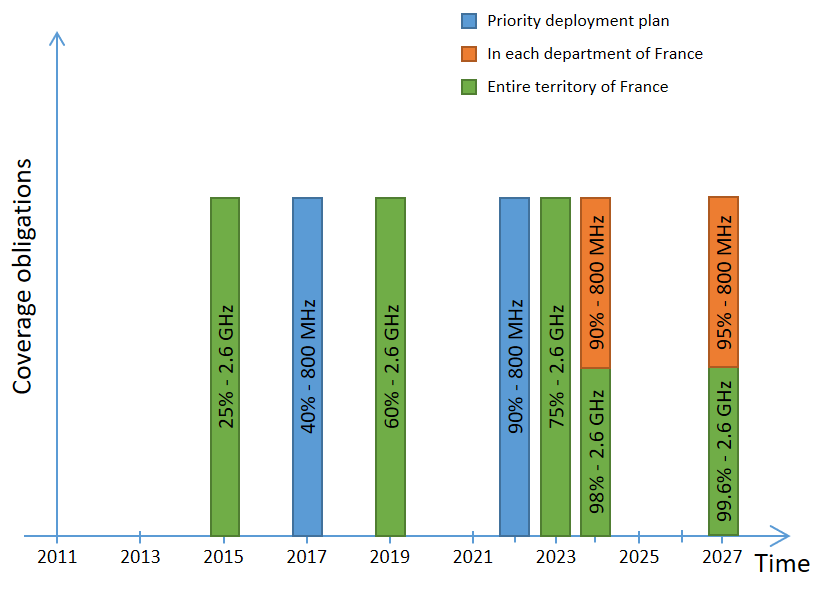
\includegraphics[width=0.95\textwidth]{./media/image12.png}
		\caption{Coverage obligations in France. Source: Author}
	\end{Center}
\end{figure}


%%%%%%%%%%%%%%%%%%%% Figure/Image No: 12 Ends here %%%%%%%%%%%%%%%%%%%%

\end{itemize}
	\item Ensure fair and effective competition in the mobile market. \textit{«the amount of spectrum that any operator will be awarded cannot exceed a 15 MHz duplex in the 800 MHz band and a 30 MHz duplex in the 2.6 GHz band. Moreover, should there be four eligible candidates for the 2.6 GHz-band frequencies, each carrier is guaranteed to receive a 15 MHz duplex if it has applied for this quantity of spectrum»}\par

	\item The proper monetization of the spectrum. To do so, the amount that candidates bid was a key criterion to win the spectrum band and each band had a minimum price to bid.
\end{itemize}\par

After the spectrum auction, Arcep published on December 22, 2011, the results of the awards procedure \cite{2-25}. These are the MNOs that won part of the spectrum:



%%%%%%%%%%%%%%%%%%%% Table No: 4 starts here %%%%%%%%%%%%%%%%%%%%


\begin{table}[H]
 			\centering
\caption{Results of the spectrum auction in France in 2011. Arcep \cite{2-25}}

\begin{tabular}{p{1.35in}p{1.35in}p{1.35in}}
\hline
%row no:1
\multicolumn{1}{|p{1.35in}}{\textbf{License recipient}} & 
\multicolumn{1}{|p{1.35in}}{\textbf{Spectrum awarded}} & 
\multicolumn{1}{|p{1.35in}|}{\textbf{Financial bid}} \\
\hhline{---}
%row no:2
\multicolumn{1}{|p{1.35in}}{Bouygues Telecom} & 
\multicolumn{1}{|p{1.35in}}{10 MHz duplex} & 
\multicolumn{1}{|p{1.35in}|}{683,087,000€} \\
\hhline{---}
%row no:3
\multicolumn{1}{|p{1.35in}}{SFR} & 
\multicolumn{1}{|p{1.35in}}{10 MHz duplex} & 
\multicolumn{1}{|p{1.35in}|}{1,065,000,000€} \\
\hhline{---}
%row no:4
\multicolumn{1}{|p{1.35in}}{Orange France} & 
\multicolumn{1}{|p{1.35in}}{10 MHz duplex} & 
\multicolumn{1}{|p{1.35in}|}{891,000,005€} \\
\hhline{---}

\end{tabular}
 \end{table}


%%%%%%%%%%%%%%%%%%%% Table No: 4 ends here %%%%%%%%%%%%%%%%%%%%

\subsection*{Germany}
\addcontentsline{toc}{subsection}{Germany}
In Germany, the policymaker responsible for regulating the telecommunication spectrum is the Bundesnetzagentur \cite{2-26} and is a federal government agency part of the German Federal Ministry of Economics and Technology (BMWi). Its main duties are the promotion of telecommunications services in public institutions, the administration of frequencies and phone numbers and the resolution of radio interferences.\par

Even though it is a national institution, Germany’s federal structure allows each federal state (Bundesland) to share some competences with the Bundesnetzagentur. Each Bundesland is responsible for regulating spectrum capacities for broadcasting purposes in its region, but the allocation of the broadcasting frequencies and the assignment process on request of capacities by the Bundesländer (plural) are a task of the national regulatory authority.\par

The process of the allocation of the 800 MHz band started on 18 February 2009, when the German Federal Cabinet announced its broadband strategy, which included a focus on making broadband access more widely available in rural areas \cite{2-27}.  After that, the Bundesrat, which is the body that represents both the Federal government and the Bundesländer, approved the Federal Cabinet decision \cite{2-28}. Finally, Bundesnetzagentur published the requirements and conditions for the allocation of the spectrum \cite{2-29}.\par

The spectrum auction started on 12 April 2010 and ended on 20 May 2010 and offered spectrum blocks from several bands:\par

\begin{itemize}
	\item 6 blocks of 2x5 MHz paired in the 800 MHz band.\par

	\item 5 blocks of 2x5 MHz paired in the 1800 MHz band.\par

	\item 8 blocks of 2x4.9 MHz paired in the 2 GHz band.\par

	\item 19.2 MHz unpaired in the 2 GHz band.\par

	\item 14 blocks of 2x5 MHz paired in the 2.6 GHz band.\par

	\item 10 blocks of 2x5 MHz unpaired in the 2.6 GHz band.
\end{itemize}\par

This auction also included significant coverage obligations only for the telecom operators that won some spectrum in the 800 MHz. Administrations of each Bundesländer defined the so-called $``$Weiße Flecken-Listen$"$  (white spot lists) and categorized villages in each Bundesland into four priority levels. For a complete list of villages for each priority and Bundesland check the following link \cite{2-30}. This way, each telecom operator can only increase the capacity of its network in an area if it has covered at least 90$\%$  of the population of the areas of the higher priority. Such connections were defined as having transmission rates of at least 1 Mbps, but due to the technical difficulties to measure a real mean download speed, the final condition is just to provide the mobile broadband connection.\par



%%%%%%%%%%%%%%%%%%%% Table No: 5 starts here %%%%%%%%%%%%%%%%%%%%


\begin{table}[H]
 			\centering
\caption{Conditions of the spectrum auction in Germany in 2010. German's Bundesnetzagentur \cite{2-30}}

\begin{tabular}{p{1in}p{2.3in}p{2in}}
\hline
%row no:1
\multicolumn{1}{|p{1in}}{\Centering \textbf{STAGE}} & 
\multicolumn{1}{|p{2.3in}}{\Centering \textbf{POPULATION SIZE}} & 
\multicolumn{1}{|p{1.7in}|}{\Centering \textbf{MIN. COVERAGE}} \\
\hhline{---}
%row no:2
\multicolumn{1}{|p{1in}}{\Centering Priority 1} & 
\multicolumn{1}{|p{2.3in}}{\Centering < 5,000 inhabitants} & 
\multicolumn{1}{|p{1.7in}|}{\Centering 90$\%$ } \\
\hhline{---}
%row no:3
\multicolumn{1}{|p{1in}}{\Centering Priority 2} & 
\multicolumn{1}{|p{2.3in}}{\Centering > 5,000 inhabitants \par \Centering < 20,000 inhabitants} & 
\multicolumn{1}{|p{1.7in}|}{\Centering 90$\%$ } \\
\hhline{---}
%row no:4
\multicolumn{1}{|p{1in}}{\Centering Priority 3} & 
\multicolumn{1}{|p{2.3in}}{\Centering > 20,000 inhabitants \par \Centering < 50,000 inhabitants} & 
\multicolumn{1}{|p{1.7in}|}{\Centering 90$\%$ } \\
\hhline{---}
%row no:5
\multicolumn{1}{|p{1in}}{\Centering Priority 4} & 
\multicolumn{1}{|p{2.3in}}{\Centering > 50,000 inhabitants} & 
\multicolumn{1}{|p{1.7in}|}{\Centering 90$\%$ } \\
\hhline{---}

\end{tabular}
 \end{table}


%%%%%%%%%%%%%%%%%%%% Table No: 5 ends here %%%%%%%%%%%%%%%%%%%%

The following chart represents the allocation made in the spectrum auction of 2010. In the 800 MHz band, three operators won spectrum: Deutsche Telekom, Telefónica O2, and Vodafone. All of them received the same amount of spectrum and the same coverage obligations.


%%%%%%%%%%%%%%%%%%%% Figure/Image No: 13 starts here %%%%%%%%%%%%%%%%%%%%

\begin{figure}[H]
	\begin{Center}
		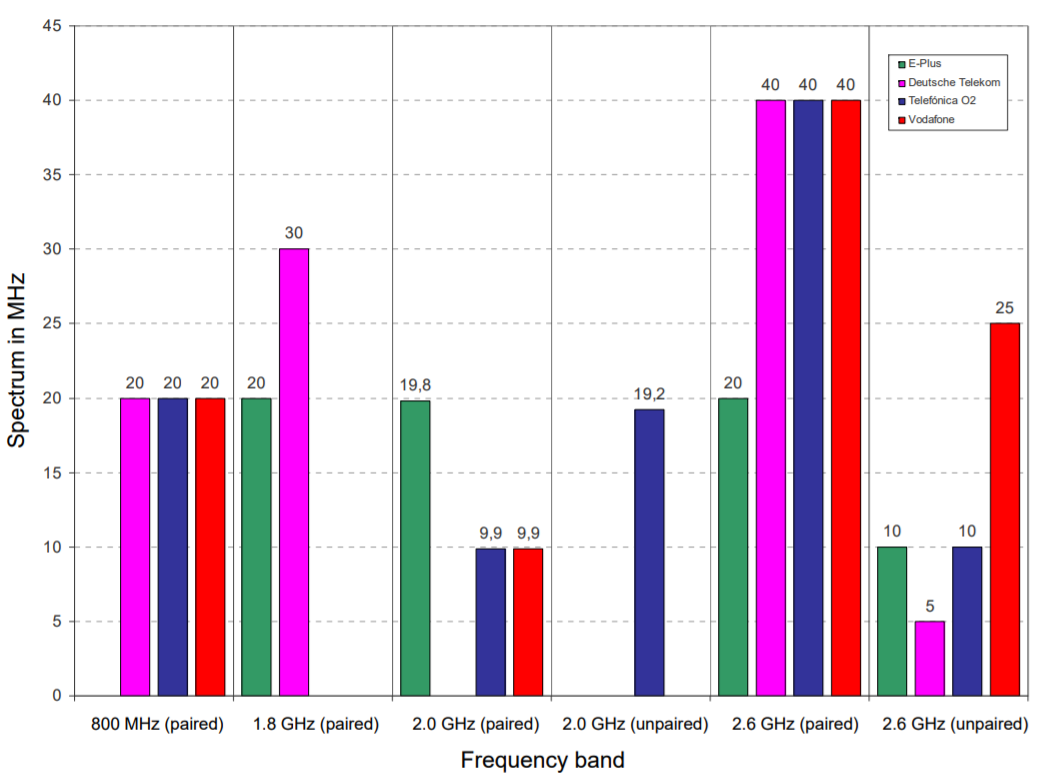
\includegraphics[width=0.95\textwidth]{./media/image13.png}
		\caption{Allocation of spectrum in the German auction of 2010. German's Bundesnetzagentur\cite{2-32}}
	\end{Center}
\end{figure}

%%%%%%%%%%%%%%%%%%%% Figure/Image No: 13 Ends here %%%%%%%%%%%%%%%%%%%%

Finally, on 26 November 2012, the Bundesnetzagentur announced that \textit{«The mobile phone companies have now fulfilled the coverage obligations in the 800 MHz range. The three companies Telekom Deutschland, Vodafone and Telefónica Germany can now freely use the frequencies they have purchased in the 800 MHz band in all federal states»} \cite{2-31}.\par


 %%%%%%%%%%%%  Starting New Page here %%%%%%%%%%%%%%
%\newpage
\vspace{\baselineskip}\chapter{Methodology: MINERVA framework}
%\addcontentsline{toc}{section}{Methodology: MINERVA, a Mobile INfrastructuRe EVAluation framework}
The Infrastructure Transitions Research Consortium (ITRC) \cite{3-01} is a research consortium of seven UK universities working on the development of tools for a national infrastructure system-of-systems model (NISMOD) \cite{3-02}. This project is modelling several national infrastructure sectors, such as digital communications, energy, and water supply, to create a common platform to help governments, utility providers, investors, and policymakers to evaluate the performance and impact of long-term plans.\par
The project is divided into several fields of study: Complex adaptative systems, databases, demographics, digital communications, economic impacts, governance, infrastructure systems, network risk analysis and solid waste.



%%%%%%%%%%%%%%%%%%%% Figure/Image No: 14 starts here %%%%%%%%%%%%%%%%%%%%

\begin{figure}[H]
	\begin{Center}
		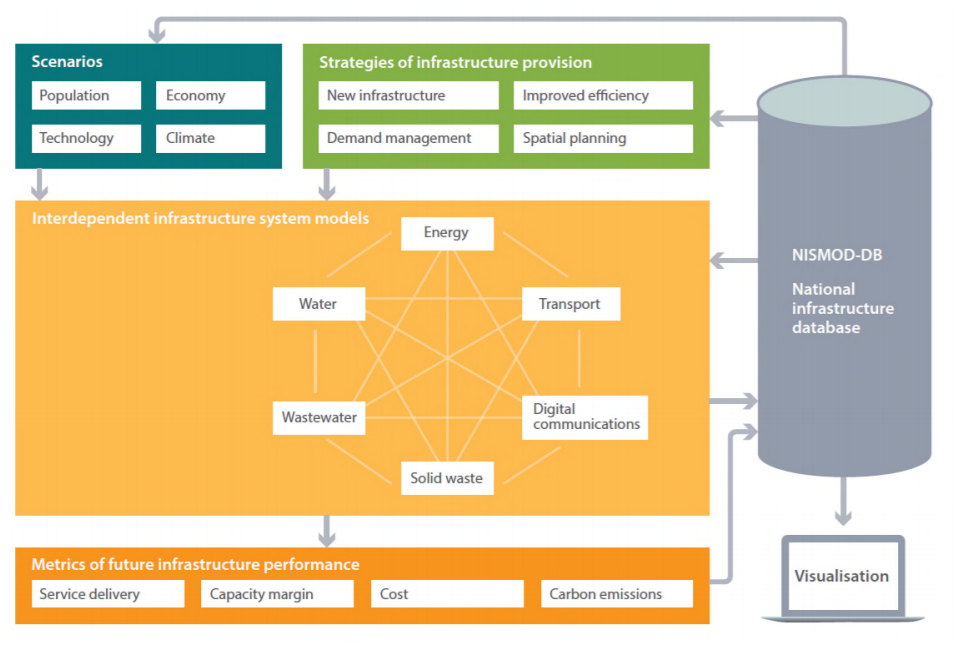
\includegraphics[width=1\textwidth]{./media/image14.png}
		\caption{The NISMOD system-of-systems model. ITRC-MISTRAL architecture\cite{3-12}}
	\end{Center}
\end{figure}


%%%%%%%%%%%%%%%%%%%% Figure/Image No: 14 Ends here %%%%%%%%%%%%%%%%%%%%

For this Master Thesis, I have used the digital communications model, available on GitHub \cite{3-04} under the MIT License, which allows «to deal with the Software without restriction, including without limitation the rights to use, copy, modify, merge, publish, distribute, sublicense, and/or sell copies of the Software». The code that was present in the repository when this thesis started is after the commit f80ce46d20deffd4d96a171e8030e98ce5d4ba02 \cite{3-09}.\par

In \cite{3-03}, Oughton, Edward et al. use the NISMOD project to quantify the uncertainty of future demand scenarios and measure the performance of different infrastructure interventions. This work uses the MINERVA (Mobile INfrastructuRe EVAluation) framework, which is under the NISMOD project, to test which infrastructure intervention strategies will be enough to meet the demand according to different demand growth rates.\par







\section{Original model}
%\addcontentsline{toc}{section}{Original model}
The following block diagram represents the structure of the project at the beginning of this Master Thesis. NISMOD stores all the information about regions and assets as well as projections of the evolution of the capacity and the demand in the UK and, given the preferred spectrum bands to use, the model can estimate how mobile network infrastructure will play out for different future scenarios.
%%%%%%%%%%%%%%%%%%%% Figure/Image No: 15 starts here %%%%%%%%%%%%%%%%%%%%
\begin{figure}[H]
	\begin{Center}
		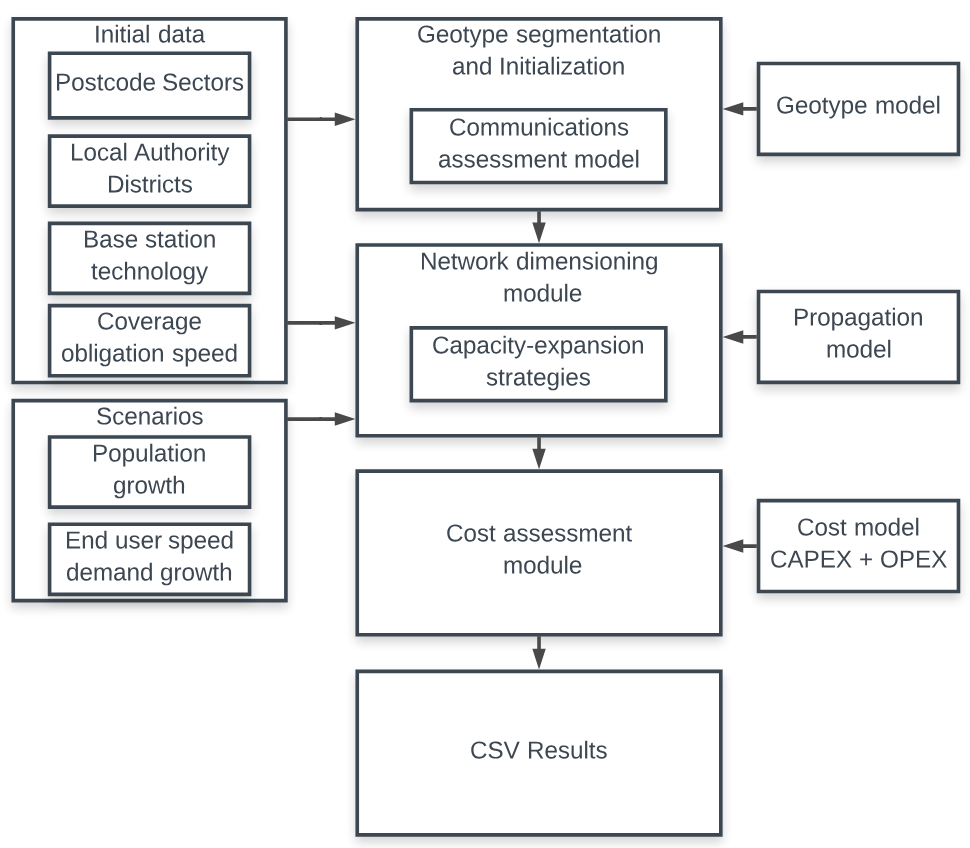
\includegraphics[width=0.95\textwidth]{./media/image15.png}
		\caption{NISMOD architecture\cite{3-03}}
	\end{Center}
\end{figure}
%%%%%%%%%%%%%%%%%%%% Figure/Image No: 15 Ends here %%%%%%%%%%%%%%%%%%%%
Population and end user speed demand projections are estimated using projection models, but only until 2030, since the accuracy of the projection decreases for longer periods. This project is capable of reporting costs and the capacity margin in each region at the end of each year. \par

\subsection{Initial data}
The project loads some scenario information at start time. This information is essential to define the environment where the simulations will take place. To assess the deployment of new assets, the code needs information about regions in which the country is divided, population and population density of the areas, and the initial assets present in the country at the beginning of the simulation. \par

\subsubsection*{Postcode Directory (PCD)}
%\addcontentsline{toc}{subsubsection}{Postcode Directory (PCD)}
It is the minimal geographical unit in the project and contains information about the population and the area in square meters. There are 8985 PCDs. The Cambridge model contains no information about Northern Ireland, and for this reason, results will only contain information about England, Scotland, and Wales.\par

\subsubsection*{Local Authority District (LAD)}
%\addcontentsline{toc}{subsubsection}{Local Authority District (LAD)}
A LAD is a group of PCDs. As there is no standard definition of LAD partitions, there are two types of LADs in the project: some which are used only for computational purposes and the ones used to generate the colour maps for the visualization module. There are 174 LADs when the information is represented on the maps.\  LADs are initialized with a list of PCDs that belong to the given LAD.\par


\subsubsection*{Initial assets}
%\addcontentsline{toc}{subsubsection}{Initial assets}
The code also loads all the information regarding assets that are already installed in the country. This is used to know the capacity of the network at the beginning and to be able to compute the capacity margin at the end of the year. For each asset, the model knows which technologies and frequencies it uses, in which PCD is, when was it built, and the spectrum bandwidth that it can use.\par


\subsubsection*{Investment}
%\addcontentsline{toc}{subsubsection}{Investment}
Investment of the telecommunications industry in the maintenance and development of the cellular networks is approximately £2 billion per year according to \cite{3-06}. In the model, this amount is divided proportionally to the market share. The market share of the telecom operator chosen for the tests is 30$\%$  which is the typical market share that the incumbent telecom operator has in a 4 telecom operators scenario, such as Spanish and British scenarios.\par


\subsubsection*{Coverage obligation}
%\addcontentsline{toc}{subsubsection}{Coverage obligation}
This version of the code has a really simple way of leading with coverage obligations. It fixes a threshold for coverage obligations, which is predefined as 10 Mbps/km\textsuperscript{2} independently of the population of the postcode which is not how Ofcom sets coverage obligations.\par


\subsubsection*{Simulation options}
%\addcontentsline{toc}{subsubsection}{Simulation options}
The model allows choosing between several scenarios to test the influence that each parameter has on the outputs. All of the parameters are explained in higher detail in the following sections, but a shorter description is:\par

\begin{itemize}
	\item \textit{pop\_scenario} which represent the rate at which the population growths. There are four options: static, low, medium, high. It is explained in section C. Scenario projections.\par

	\item \textit{throughput\_scenario} which represents how the demand per user growths over time. There are three options: low, medium, high. It is explained in section C. Scenario projections.\par

	\item \textit{intervention\_strategy }which represent the specific interventions that are allowed in this run. There are four options: Minimum intervention, Spectrum integration strategy, small cells strategy, and Hybrid strategy. It is explained in section D. Network dimensioning module.\par
\end{itemize}

\subsection{Geotype segmentation and initialization}
This module takes all the information loaded at start time and computes MINERVA, the \textit{«Mobile INfrastructuRe EVAluation framework». }MINERVA is an object that contains the current information about all the regions and updates it when there are changes in the population information or when a new asset is built. \par

\subsubsection*{Geotype model}
%\addcontentsline{toc}{subsubsection}{Geotype model}
PCDs are segmented into geotypes when they are added to the CCAM. Geotypes are used to perform a more granular analysis of the rollout and represent the key supply-side variables that affect the rollout costs. This project uses the categorization that Analysis Mason used in \cite{3-011} for Ofcom. The module segments areas with similar characteristics, such as similar population density, and classify the regions into three main types: urban, suburban and rural. Each main type is then subdivided into one or more geotypes, and the full picture of the UK with the distribution of the geotypes around the country is shown in the following figure:
%%%%%%%%%%%%%%%%%%%% Figure/Image No: 16 starts here %%%%%%%%%%%%%%%%%%%%
\begin{figure}[H]
	\begin{Center}
		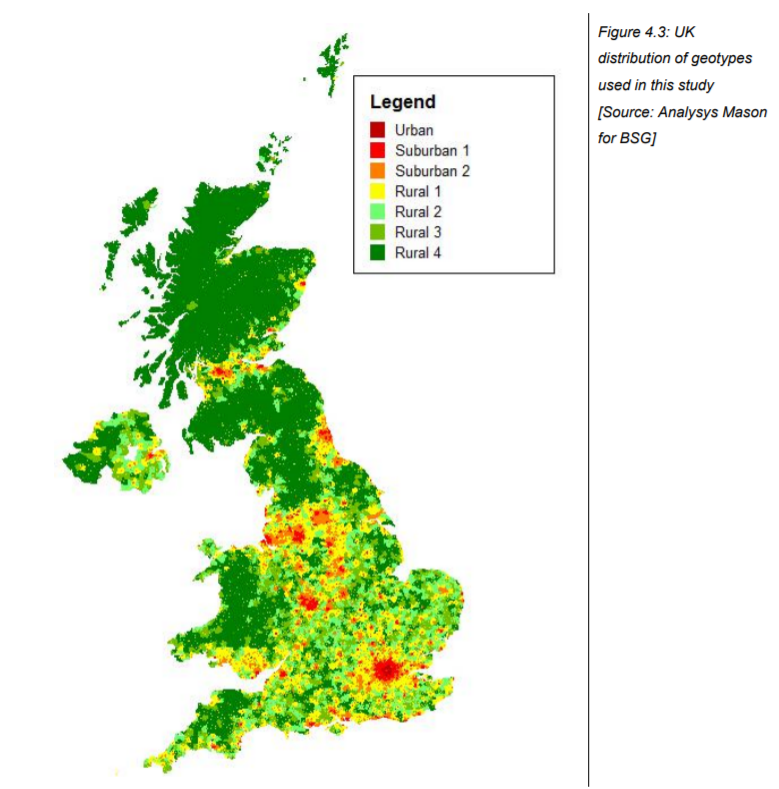
\includegraphics[width=0.7\textwidth]{./media/image16.png}
		\caption{Geotypes in the UK. Analysis Mason\cite{3-11}}
	\end{Center}
\end{figure}
%%%%%%%%%%%%%%%%%%%% Figure/Image No: 16 Ends here %%%%%%%%%%%%%%%%%%%%
For the sake of simplicity, NISMOD divides regions into the three main geotypes: Urban, suburban and rural. (I) When the population density is at least 7,959 inhabitants per square meter, the area is considered of geotype Urban. This occurs approximately on 0.2$\%$  of the area of Britain and 8.3$\%$  of the population. (II) The second type is Suburban and is for regions with population density from 782 to 7,958 inhabitants per square meter. This region covers 7$\%$  of the area and 61$\%$  of the population. (III) Finally, the rural area is for regions with lower population densities and covers 92$\%$  of Britain’s size, but just 29$\%$  of the population.\par

Despite some PCDs being considerably homogeneous, most of them contain some parts that could be categorized as urban, suburban and rural. We do not have such detailed database to perform that analysis and, therefore, some areas could be miscategorized. For example, a PCD with 4,000 inhabitants and 1km\textsuperscript{2} would be considered suburban, but if the population is living in just the 50$\%$  of the area, the site density of the urban part is 8,000, so it would be categorized as 50$\%$  urban and 50$\%$  rural (If nobody lives in this part). This issue cannot be resolved with the current data of the model because the percentage of the area where inhabitants live over the total varies significantly in each PCD.
%%%%%%%%%%%%%%%%%%%% Figure/Image No: 17 starts here %%%%%%%%%%%%%%%%%%%%
\begin{figure}[H]
	\begin{Center}
		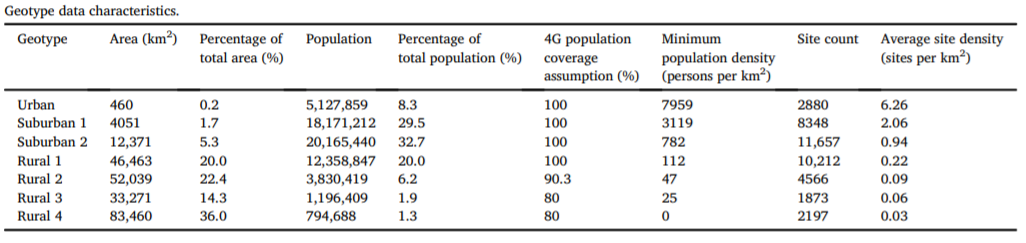
\includegraphics[width=1.1\textwidth]{./media/image17.png}
		\caption{Geotypes data characteristics. Edward J. Oughton and Zoraida Frias\cite{3-03}}
	\end{Center}
\end{figure}
%%%%%%%%%%%%%%%%%%%% Figure/Image No: 17 Ends here %%%%%%%%%%%%%%%%%%%%
\subsection{Scenario projections}
Two main projections are used in this project: the estimation of the growth of the population and the calculation of the demand for download speed from 2020 to 2030. Two are the reasons why 2030 is the last year of the projections: (I) Population trend may vary a lot in the years to come - check the following link with population projections prepared by the United Nations \cite{3-07} – so it makes no sense to predict data for more than 10 years. End-user speed may vary even more drastically than population. (II) Telecommunication technologies evolve quite fast and considering that there will not appear new technologies in more than 10 years is a conservative planning approach that may not occur.
%%%%%%%%%%%%%%%%%%%% Figure/Image No: 18 starts here %%%%%%%%%%%%%%%%%%%%
\begin{figure}[H]
	\begin{Center}
		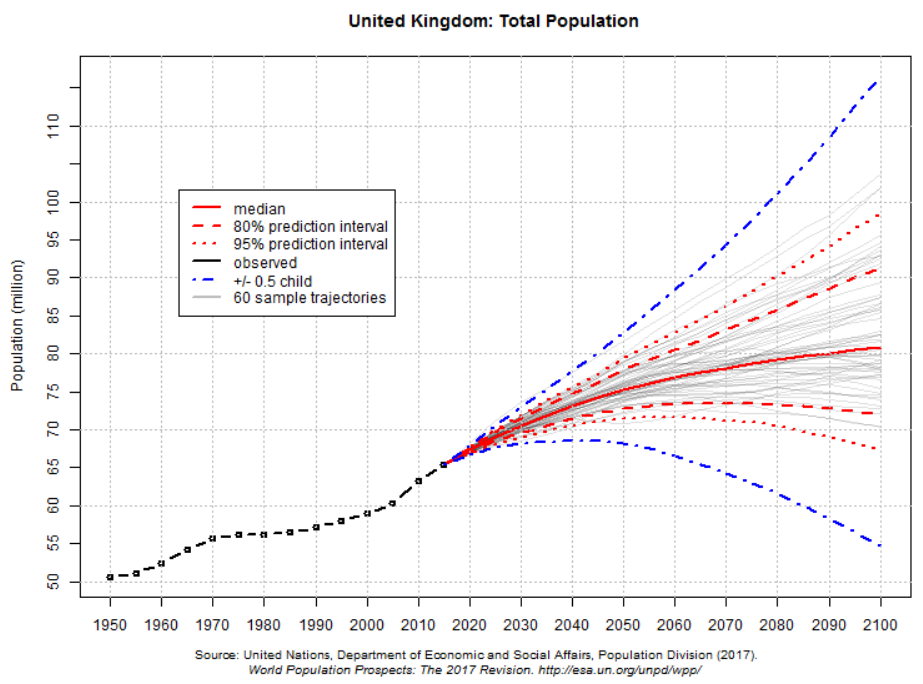
\includegraphics[width=0.8\textwidth]{./media/image18.png}
		\caption{Projections of the population in the UK. United Nations\cite{3-13}}
	\end{Center}
\end{figure}
%%%%%%%%%%%%%%%%%%%% Figure/Image No: 18 Ends here %%%%%%%%%%%%%%%%%%%%
\subsubsection*{Population projections}
%\addcontentsline{toc}{subsubsection}{Population projections}
Data of the population of each PCD has been taken from the UK Census. As Scotland has not published more population data since 2011, the data used in the project is taken from the 2011 Census and then aggregated for each PCD. The population growth model is in the NISMOD GitHub, but outside the digital\_comms repository, as it is used for all the Interdependent infrastructure system models. The repository \cite{3-08} allows creating several projections depending on the fertility, life expectancy, migration, future EU migration and other factors. In this thesis, the population for the following years is modelled according to four different approximations depending on the growing rate forecasted: $``$Static$"$ , $``$low$"$ , $``$medium$"$  and $``$high$"$.



%%%%%%%%%%%%%%%%%%%% Figure/Image No: 19 starts here %%%%%%%%%%%%%%%%%%%%

\begin{figure}[H]
	\begin{Center}
		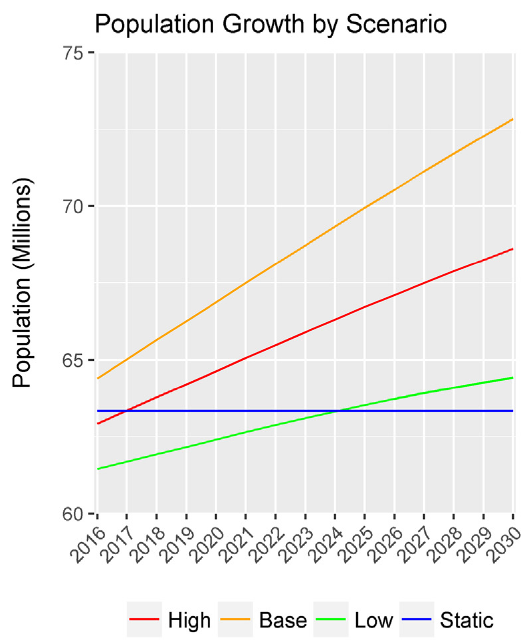
\includegraphics[width=0.60\textwidth]{./media/image19.png}
		\caption{Population scenarios. NISMOD\cite{3-07}}
	\end{Center}
\end{figure}
%%%%%%%%%%%%%%%%%%%% Figure/Image No: 19 Ends here %%%%%%%%%%%%%%%%%%%%
For a deeper explanation, please refer to the following paper \cite{3-03}.

\subsubsection*{End-user speed projections}
%\addcontentsline{toc}{subsubsection}{End-user speed projections}
Demand in each PCD is part of the outputs of this project, but results may vary depending on the model used. Demand projections are estimated in data consumption per month and per user. As in the population projections, the demand growth rate is not included in the source code, but the model is perfectly parametrized, so new estimations can be added. \par

The Cisco VNI white paper \cite{3-08} has been used to estimate the end-user speed demand. Their report for 2016-2021 states that: «Mobile network connection speeds will increase threefold by 2021. The average mobile network connection speed (6.8 Mbps in 2016) will reach 20.4 megabits per second (Mbps) by 2021» and «The average smartphone will generate 6.8 GB of traffic per month by 2021, a fourfold increase over the 2016 average of 1.6 GB per month. By 2021, aggregate smartphone traffic will be seven times greater than it is today, with a CAGR of 48 per cent».



%%%%%%%%%%%%%%%%%%%% Figure/Image No: 20 starts here %%%%%%%%%%%%%%%%%%%%

\begin{figure}[H]
	\begin{Center}
		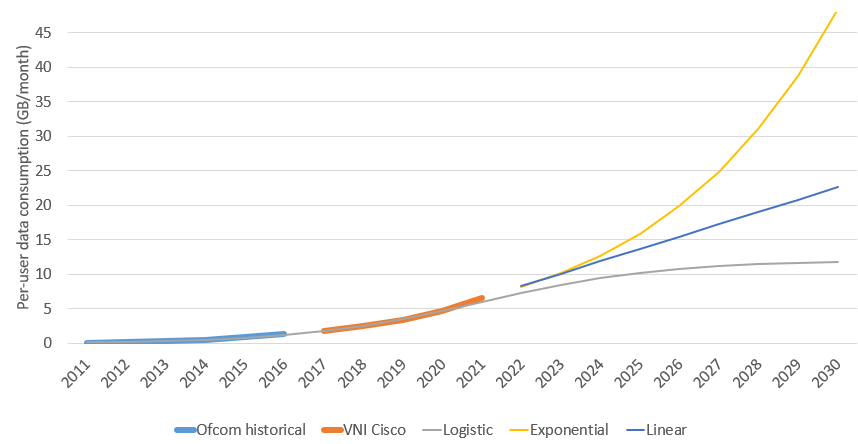
\includegraphics[width=0.9\textwidth]{./media/image20.png}
		\caption{End-user speed demand in the busy hour projections. NISMOD\cite{3-07}}
	\end{Center}
\end{figure}


%%%%%%%%%%%%%%%%%%%% Figure/Image No: 20 Ends here %%%%%%%%%%%%%%%%%%%%


This thesis uses three different models to estimate the variation of the demand across the years:\par

\begin{itemize}
	\item Logistic approximation which in the visualization model is named as $``$low$"$ . This scenario is the $``$worst$"$  for the 5G adoption, as it would mean that no killer app or data consumption model has appeared to change the way people use broadband data services.\par

	\item Linear evolution which is named $``$medium$"$  in the visualization model.\par

	\item Exponential evolution of the data consumption at 25$\%$  Compound annual growth rate over 2021-2030 which is named as $``$high$"$ .
\end{itemize}

\vspace{\baselineskip}


%%%%%%%%%%%%%%%%%%%% Figure/Image No: 21 starts here %%%%%%%%%%%%%%%%%%%%

\begin{figure}[H]
	\begin{Center}
		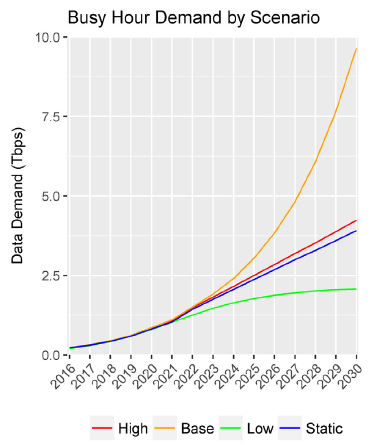
\includegraphics[width=0.60\textwidth]{./media/image21.png}
		\caption{End-user speed demand in the busy hour projections. NISMOD\cite{3-07}}
	\end{Center}
\end{figure}


%%%%%%%%%%%%%%%%%%%% Figure/Image No: 21 Ends here %%%%%%%%%%%%%%%%%%%%

Once the models are introduced into the program, the demand is transformed from GB per month per user to Mbps per user in the busy hour. The formula used is:\par
\begin{multline*}
Demand\_in\_mbps = Demand\_in\_GB \\ $\ast$ 1024 $\ast$ 8 $\ast$ percentage / 30 / 3600 
\end{multline}

where percentage is the percentage of the traffic in the busy hour. It is estimated as 7.5$\%$ of the total traffic of the day.\par



\subsection{Network dimensioning module}
For each year, as long as there is enough budget for more investments, the project checks the PCDs in order, from more densely populated areas to less, looking for PCDs where the demand is higher than the capacity installed. This module is called once per year and PCD and triggers the suggest\_intervention function every time there is a lack of capacity in a PCD in the given year. This function checks the intervention options allowed in the PCD and builds the assets that the PCD needs to reach the capacity.\par

The model uses the capacity lookup table to calculate the capacity installed and the extra capacity provided by the new assets. The model has also several predefined interventions which are basically one per technology and capacity-expansion strategies, which are the set of interventions that are allowed in each simulation.\par

\subsubsection*{Propagation model}
%\addcontentsline{toc}{subsubsection}{Propagation model}
The propagation model is a set of curves that estimate the capacity per area unit of the PCD depending on the site density (only considering assets that have the same frequency and technology), the frequency, bandwidth and technology and the geotype of the given PCD \cite{3-09}.\par

Each capacity curve is calculated using several cell parameters, such as the macrocellular layout, the frequency reuse factor, the cell-edge, the overbooking factor, etc. A comprehensive study of how all these factors influence in the network capacity can be checked in \cite{3-10}. The following table represents all the parameters considered in the estimations:



%%%%%%%%%%%%%%%%%%%% Figure/Image No: 22 starts here %%%%%%%%%%%%%%%%%%%%

\begin{figure}[H]
	\begin{Center}
		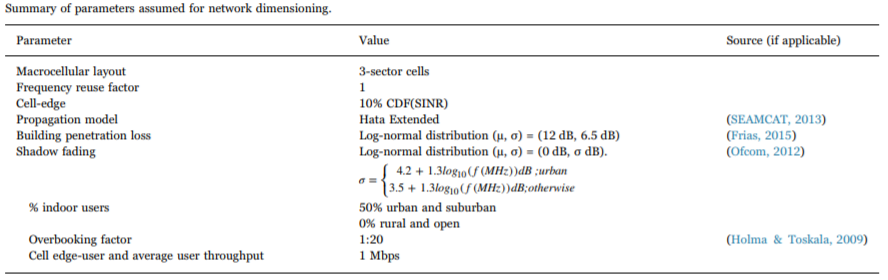
\includegraphics[width=1.05\textwidth]{./media/image22.png}
		\caption{Network dimensioning parameters. Zoraida Frias\cite{3-14}}
	\end{Center}
\end{figure}


%%%%%%%%%%%%%%%%%%%% Figure/Image No: 22 Ends here %%%%%%%%%%%%%%%%%%%%

%\vspace{\baselineskip}
%\textbf{Aquí hay que hablar sobre las tablas de propagación:}\par
%
%
%
%%%%%%%%%%%%%%%%%%%%% Figure/Image No: 23 starts here %%%%%%%%%%%%%%%%%%%%
%
%\begin{figure}[H]
	%\begin{Center}
		%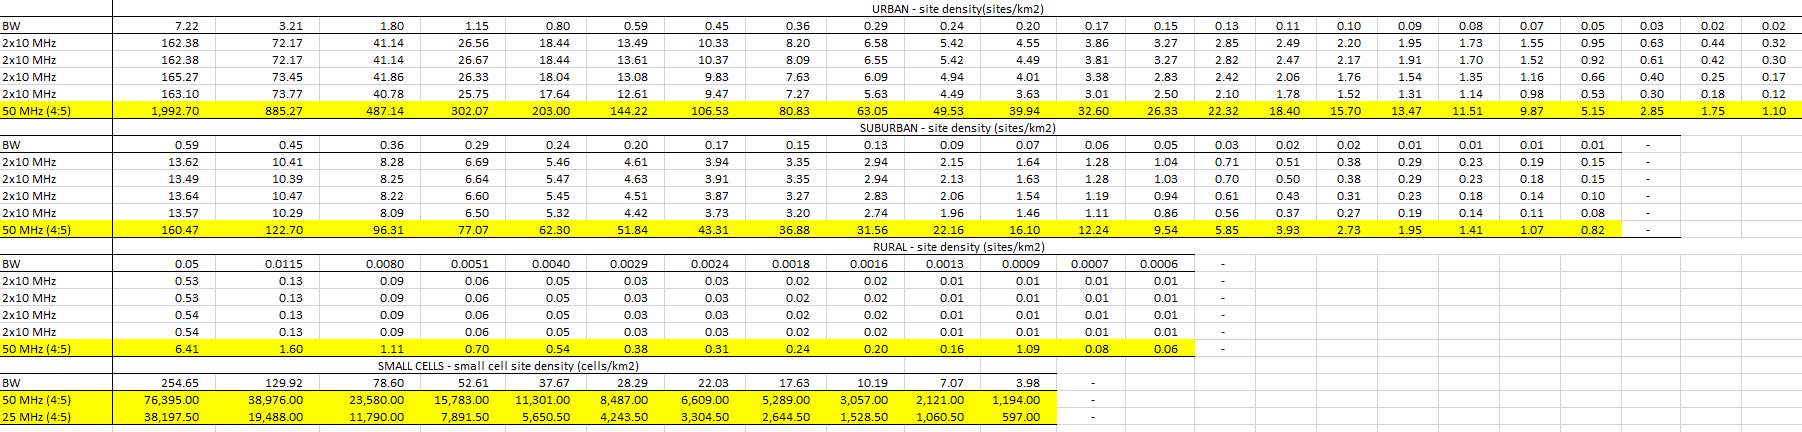
\includegraphics[width=6.5in,height=1.56in]{./media/image23.png}
		%\caption{}
	%\end{Center}
%\end{figure}
%
%
%%%%%%%%%%%%%%%%%%%%% Figure/Image No: 23 Ends here %%%%%%%%%%%%%%%%%%%%
%
%\textbf{ }\par
%
%\textbf{De alguna manera hay que explicar que las regiones rurales tienen una capacidad máxima menor y cosas así.}\par

\subsubsection*{Interventions}
%\addcontentsline{toc}{subsubsection}{Interventions}
There are four intervention types defined in the Network Dimensioning model. Each of them implies normally the usage of one specific technology but choosing one does not directly prevent the telecom operator from using the rest. The possible interventions in the original model where:\par

\begin{itemize}
	\item $``$Upgrade site to LTE$"$ : This intervention is available for every already built asset that has only 2G and 3G. When it is possible to build more than one intervention, this one has a higher priority than the rest. This intervention is a combination of building: (I) 800 MHz carrier with LTE technology and 2x10 MHz (II) 2600 MHz carrier with LTE technology and 2x10 MHz in the same place were the original asset was.\par

	\item $``$Build 700 MHz carrier$"$ : This intervention is only possible in those sites that do not emit in 700 MHz yet, but has already performed the upgrade to LTE intervention. It can be built only from 2020 onwards since this is the carrier that will be allocated to telecommunications in most European countries after the second digital dividend. This intervention builds a 700 MHz carrier of 2x10 MHz in the same place where the original asset was.\par

	\item $``$Build 3500 MHz carrier$"$ : This intervention is only possible in those sites that do not emit in 3500 MHz yet, but has already performed the upgrade to LTE intervention. As the 700 MHz band, it can be built only from 2020 onwards because it is the 3.4 GHz band that was awarded in April 2018 with the aim of using it for 5G services. This intervention builds a 3500 MHz carrier of 50 MHz in the same place where the original asset was.\par

	\item $``$Build a small cell$"$ : This intervention builds a new site in a place that does not necessarily need to have a previous macrocell asset built. It builds a small cell asset with 5G technology, in the band of 3700 MHz and with a bandwidth of 2x25 MHz. This type of assets cannot be built until 2020 for the same reason as the previous ones.\par

It is worth noting that 900 MHz, 1800 MHz, and 2100 MHz are excluded from the current analysis as legacy networks operate on that spectrum and there is no evidence to suggest that this bands will be refarmed to 5G technologies in the midterm, at least before 2030 which is the last year of study.\par


\end{itemize}
\subsubsection*{Capacity-expansion strategies}
%\addcontentsline{toc}{subsubsection}{Capacity-expansion strategies}
Not all the situations allow building any type of intervention because maybe a specific band is not allocated for broadband services in a given country or the telecom operator tested has no spectrum allocated in this band. Capacity-expansion strategies allow creating the set of interventions that will be available in each test.\par

This mechanism also simplifies the analysis for telecom operators, since they can simulate the effects that bidding for more bandwidth in a new band will take into their budget. And even for policymakers, because they will be able to quantify the importance of a given spectrum for a specific telecom operator and the amount of money that they would be willing to pay for it. \par

Four types of strategies have been defined in this model:\par



%%%%%%%%%%%%%%%%%%%% Table No: 6 starts here %%%%%%%%%%%%%%%%%%%%


\begin{table}[H]
 			\centering
\begin{tabular}{p{1.35in}p{3.92in}}
\hline
%row no:1
\multicolumn{1}{|p{1.35in}}{\Centering \textbf{Strategy name}} & 
\multicolumn{1}{|p{3.92in}|}{\Centering \textbf{Description}} \\
\hhline{--}
%row no:2
\multicolumn{1}{|p{1.35in}}{\Centering Minimum intervention} & 
\multicolumn{1}{|p{3.92in}|}{This strategy operates and maintains existing network and does not deploy new assets in any frequency band.} \\
\hhline{--}
%row no:3
\multicolumn{1}{|p{1.35in}}{\Centering 700MHz spectrum integration} & 
\multicolumn{1}{|p{3.92in}|}{Upgrade to LTE if not available (800 MHz and 2600 MHz). \par Integrate spectrum in the 700 MHz band.} \\
\hhline{--}
%row no:4
\multicolumn{1}{|p{1.35in}}{\Centering Spectrum integration} & 
\multicolumn{1}{|p{3.92in}|}{Upgrade to LTE if not available (800 MHz and 2600 MHz). \par Integrate all another spectrum on the brownfield microcellular network (700 and 3500 MHz).} \\
\hhline{--}
%row no:5
\multicolumn{1}{|p{1.35in}}{\Centering Small cells strategy} & 
\multicolumn{1}{|p{3.92in}|}{Upgrade to LTE if not available (800 MHz and 2600 MHz). \par Deploy a greenfield small cell layer operating in TDD at 3700 MHz.} \\
\hhline{--}
%row no:6
\multicolumn{1}{|p{1.35in}}{\Centering Hybrid strategy} & 
\multicolumn{1}{|p{3.92in}|}{Upgrade to LTE if not available (800 MHz and 2600 MHz). \par Integrate all another spectrum on the brownfield microcellular network (700 and 3500 MHz). \par Deploy a greenfield small cell layer operating in TDD at 3700 MHz.} \\
\hhline{--}

\end{tabular}
\caption{Capacity expansion strategies. NISMOD}
 \end{table}


%%%%%%%%%%%%%%%%%%%% Table No: 6 ends here %%%%%%%%%%%%%%%%%%%%


\vspace{\baselineskip}
\subsection{Cost assessment module}
Every time the network dimensioning module builds a new intervention, the cost assessment module is triggered to store the type of intervention, the year and how much does this specific intervention cost. This way the model knows how much has been spent in the current year and if there is enough budget for more interventions. The cost assessment module uses a cost model which is explained in higher detail in the following paper \cite{3-03}.\par

\subsubsection*{Cost model}
%\addcontentsline{toc}{subsubsection}{Cost model}
The cost of each intervention can be calculated using the following formula:\par

 \[ Total\_cost\_of\_an\_intervention = CAPEX + OPEX \] \par

The Capital Expenditures (CAPEX) of the $``$upgrade to LTE$"$  intervention is the cost of deploying a multicarrier BS (£40,900) plus the cost of the civil works (£18,000). As the multicarrier base station lifetime is estimated at 10 years and the original project runs from 2017, two multicarrier base stations are needed. The Operational Expenditures (OPEX) of the $``$upgrade to LTE$"$  intervention is £3,898 per year. To aggregate all of these costs, the present value of the future cash flow has been calculated using a discount rate of 3.5$\%$  and the total cost is estimated at £142,446.\par

The cost calculated for the strategies $``$700 MHz integration$"$  and $``$3500 MHz integration$"$  is the same because these strategies can only be undertaken if there is an existing LTE base station in the list of assets. Therefore, the cost of deploying a multicarrier base station (£40,900) is reduced to only installing an additional carrier on the current base station, which is only £15,000. The OPEX is also reduced to £1,800 and therefore, the total cost discounted to the present value is £50,917.\par

Lastly, the cost of the small cell strategy is calculated using the CAPEX plus OPEX formula, but in this case, the small cell is expected to have only 5 years of lifetime, so 4 small cells have to be built. Each small cell equipment is £2,500 and the civil works (which are needed just the first time) are £13,300. Opex is calculated as the OPEX of the small cell equipment (£350) plus the £1,000 of backhaul OPEX. The total amount that this intervention costs discounted to the present value is £40,220.\par

A summary of the costs of each asset is made based on the following table that was extracted from \cite{3-10}:



%%%%%%%%%%%%%%%%%%%% Figure/Image No: 24 starts here %%%%%%%%%%%%%%%%%%%%

\begin{figure}[H]
	\begin{Center}
		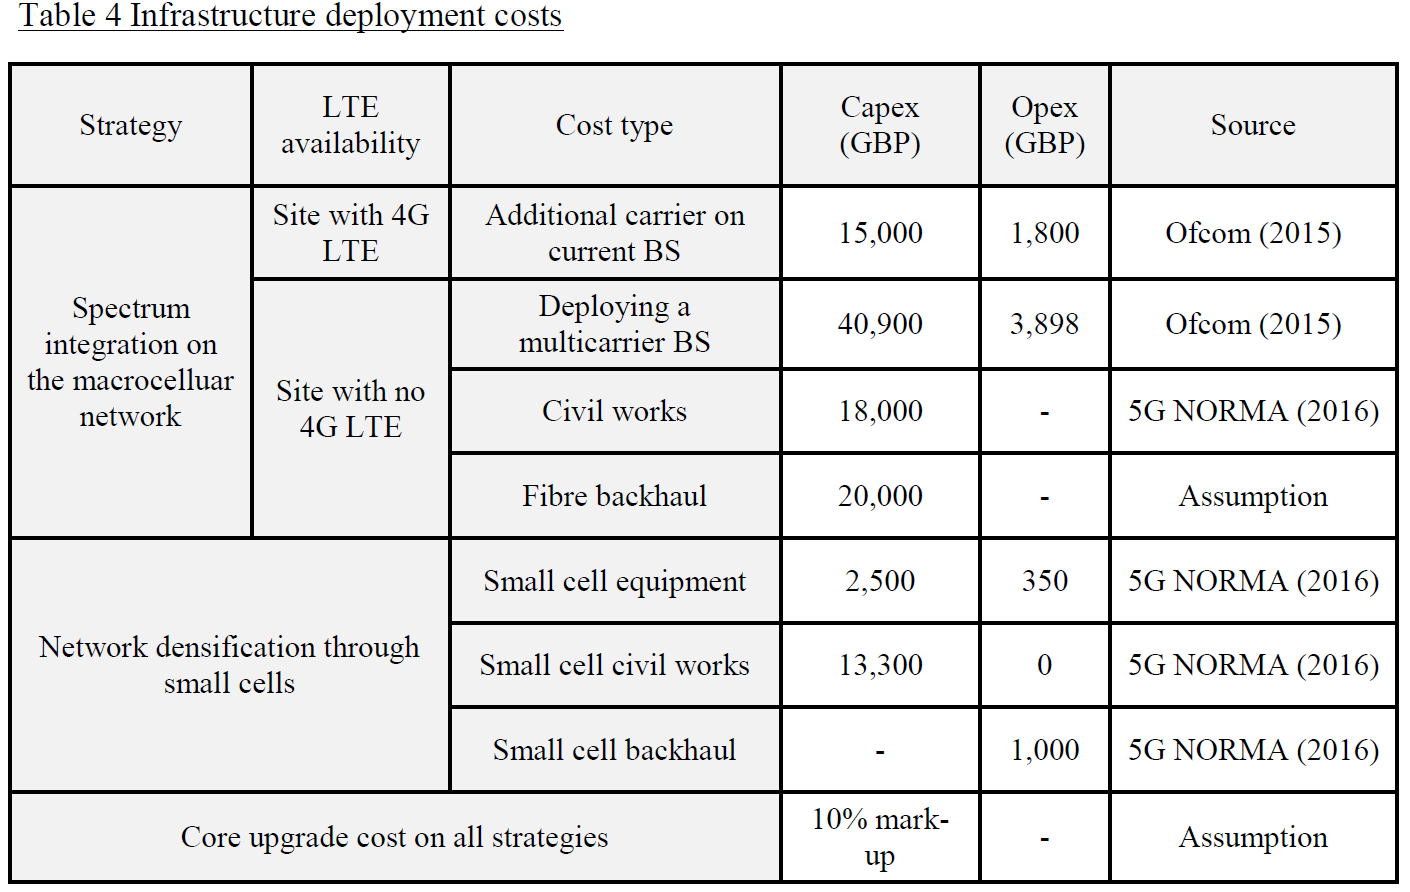
\includegraphics[width=0.95\textwidth]{./media/image24.png}
		\caption{Infrastructure deployment costs. NISMOD\cite{3-10}}
	\end{Center}
\end{figure}


%%%%%%%%%%%%%%%%%%%% Figure/Image No: 24 Ends here %%%%%%%%%%%%%%%%%%%%


\subsection{Model results}
This section describes the outcomes of the original model. The outputs are grouped in three types of .csv files in the outputs folder. Each of them provides the following information:\par

\begin{itemize}
	\item Decisions.csv provides information about the assets that were built in the simulation and their related information: in which year, in which PCD and specific asset (all the interventions, except small cells, are built at existing sites), the type and technology of the installation and the frequency and bandwidth.\par

	\item Metrics.csv and pcd\_metrics.csv provide information about the deployment situation after the network dimensioning module algorithm has been run for each year. The metrics.csv file gives information of the LADs and the pcd\_metrics.csv file gives information of the PCDs. The information of each PCD and LAD is total demand per km\textsuperscript{2}, total capacity per km\textsuperscript{2}, capacity deficit per km\textsuperscript{2}, population and population density.\par

	\item Spend.csv provides information about the interventions built and the cost that their cost.\par

This is all the information that the model outputs provide. The rest of the information has to be calculated or represented using external tools that are not included.\par


\end{itemize}
\subsubsection*{Timeframe}
%\addcontentsline{toc}{subsubsection}{Timeframe}
It is possible to know when the model decides that no more assets are needed to satisfy the data demand and the coverage obligations set by i.e. a policymaker, just by aggregating all the expenses per year and checking in which year the total sum is less than the available budget.\par

\subsubsection*{Capacity}
%\addcontentsline{toc}{subsubsection}{Capacity}
Capacity in each PCD is measured per km\textsuperscript{2} and is the result of aggregating the capacity provided by all the assets in each PCD. Representing the value of the capacity results in a figure that is not so useful, because the values in the y-axis do not have a specific shape, not as demand and capacity margin figures. For the sake of consistency and to explain the shape of the capacity margin, it can be checked below:



%%%%%%%%%%%%%%%%%%%% Figure/Image No: 25 starts here %%%%%%%%%%%%%%%%%%%%

\begin{figure}[H]
	\begin{Center}
		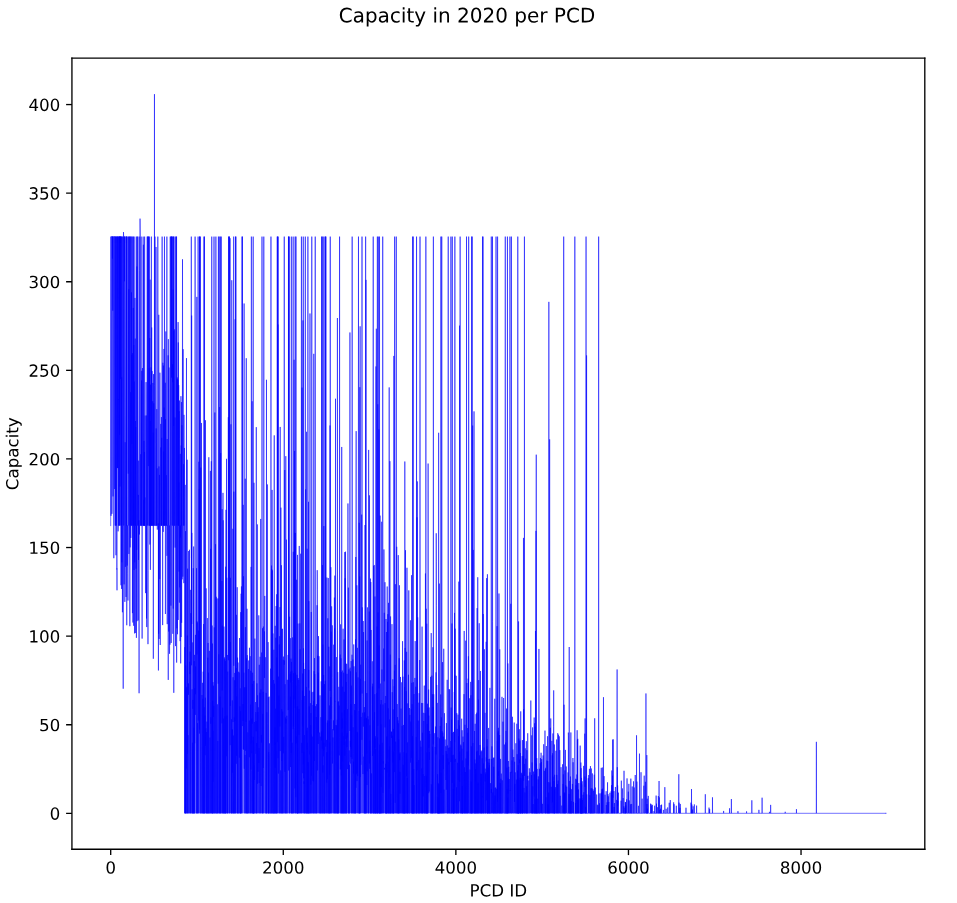
\includegraphics[width=0.95\textwidth]{./media/image25.png}
		\caption{Capacity in 2020 per PCD. Source: Author}
	\end{Center}
\end{figure}


%%%%%%%%%%%%%%%%%%%% Figure/Image No: 25 Ends here %%%%%%%%%%%%%%%%%%%%


\subsubsection*{Demand}
%\addcontentsline{toc}{subsubsection}{Demand}
The demand in each PCD is also measured per km\textsuperscript{2} and is calculated according to the rules explained in the End-user speed projections section. The resulting demand is obtained by multiplying the potential users by the demand per user and an overbooking factor that represent that not all the users are demanding network resources simultaneously.\par

 \[ Demand = users\ast demand \_ per \_ user \ast overbooking \_ factor / area \] \par

where:\par

\begin{itemize}
	\item \textit{users} is estimated multiplying the whole population of the PCD by the mobile broadband services penetration (estimated in 80$\%$ ) and by the market share of the telecom operator (in this case is 30$\%$ ).\par

	\item The \textit{overbooking\_factor} is set to 50.\par

	\item The \textit{area} is the area of each PCD.\par

	\item \textit{Demand\_per\_user} is obtained from the end-user speed demand chart and then converted from demand in GB/month to Mbps/user using the following formula:\par
\end{itemize}
\begin{Center}
\begin{multline*}
Demand \_ in \_ mbps =Demand \_ in \_ GB \ \ast \ 1024 \ \ast 8 \ast \\
 Traffic \_ in \_ busy \_ hour \ / 30 \ / 3600
\end{multline}
\end{Center}\par

Hence, graphically, \textit{Demand\_in\_Mbps} is the result of multiplying the area by the demand per user (which has one of the given functions in the projection section) by several factors and that is why the demand has the shape in the following figure:



%%%%%%%%%%%%%%%%%%%% Figure/Image No: 26 starts here %%%%%%%%%%%%%%%%%%%%

\begin{figure}[H]
	\begin{Center}
		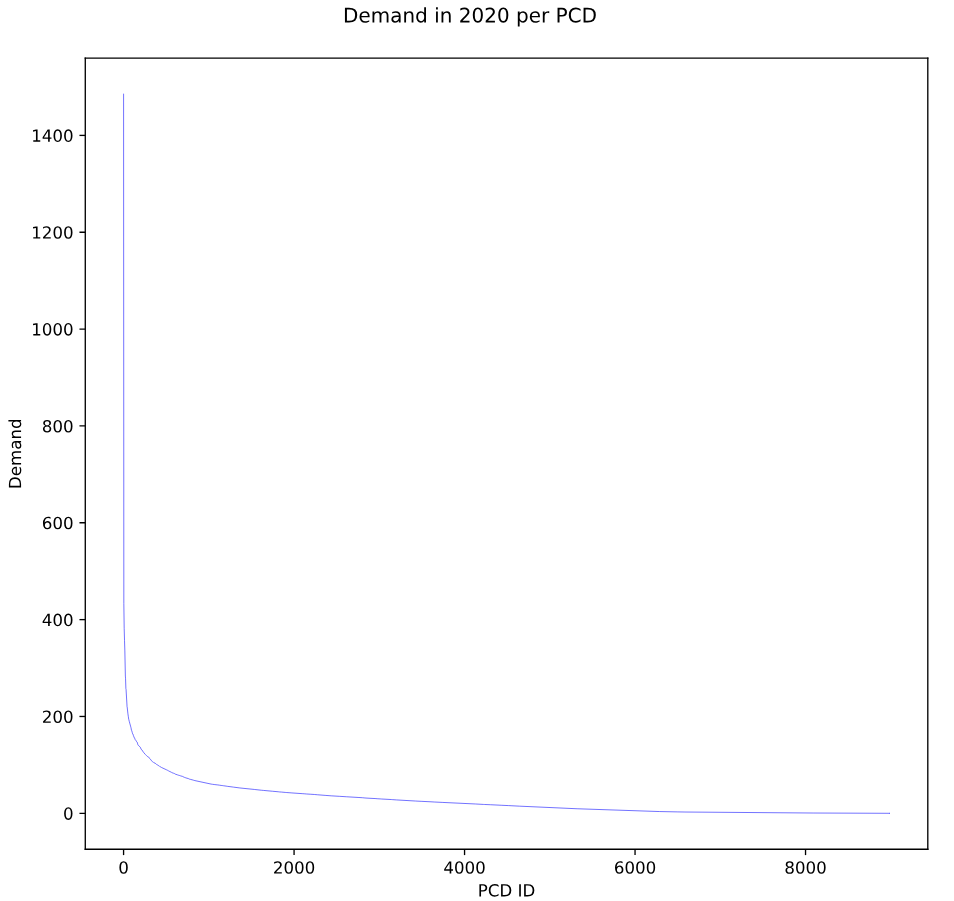
\includegraphics[width=0.95\textwidth]{./media/image26.png}
		\caption{Demand in 2020 per PCD. Source: Author}
	\end{Center}
\end{figure}


%%%%%%%%%%%%%%%%%%%% Figure/Image No: 26 Ends here %%%%%%%%%%%%%%%%%%%%



\subsubsection*{Capacity margin}
%\addcontentsline{toc}{subsubsection}{Capacity margin}
The capacity margin for a given PCD is the result of the capacity minus the demand and is measured in Mbps/km\textsuperscript{2}. In the PCDs graph, the capacity margin function is just the result of subtracting the demand function from the capacity one. Negative values represent a capacity deficit. This is the formula to calculate the capacity margin:\par

 \[ Capacity\_ margin  \left( Mbps/km^{2} \right) = Capacity  \left( Mbps/km^{2} \right)  - Demand  \left( Mbps/km^{2} \right)  \] 

%%%%%%%%%%%%%%%%%%%% Figure/Image No: 27 starts here %%%%%%%%%%%%%%%%%%%%

\begin{figure}[H]
	\begin{Center}
		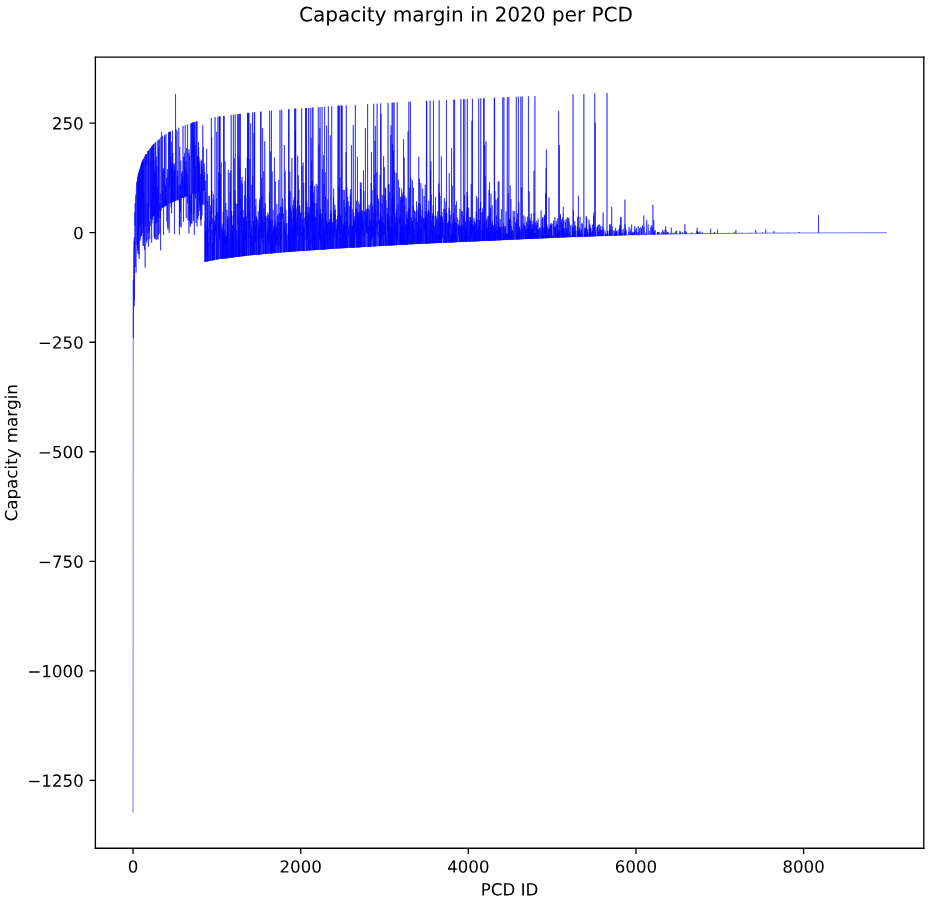
\includegraphics[width=0.95\textwidth]{./media/image27.png}
		\caption{Capacity margin in 2020 per PCD. Source: Author}
	\end{Center}
\end{figure}


%%%%%%%%%%%%%%%%%%%% Figure/Image No: 27 Ends here %%%%%%%%%%%%%%%%%%%%

\subsubsection*{Cost and capacity margin}
%\addcontentsline{toc}{subsubsection}{Cost and capacity margin}
The capacity margin is as important as costs in the model because one cannot show the whole picture without the other. A given cost is better or worst depending on if it has raised more or less the capacity margin, which is a measure of effectiveness. This fact shows the differences between urban, suburban and rural areas since rural area investments are not so efficient rising the capacity margin as investments in urban areas.\par

When comparing results from different scenarios and capacity-expansion strategies, for similar costs, better capacity margins imply better strategies a priori. And for similar capacity margins, fewer costs imply better strategies a priori.\par

When neither the capacity margin and the cost is similar, the decision of which strategy is better depends on aspects which are out of the scope of the digital comms project, because they are related to the interest of the government and stakeholders to have a universal access to broadband services in the country, the macroeconomic situation of the country, etc.\par


















 %%%%%%%%%%%%  Starting New Page here %%%%%%%%%%%%%%
%\vspace{\baselineskip}
\section{Contribution to the project}
%\addcontentsline{toc}{subsection}{Contribution to the project}
The following diagram shows the previous state of the project and the green boxes represent the modules that have been further developed in this Master Thesis. The first contribution to the project, and the one that enabled the rest of them was the creation of a data management structure to store some of the environment options and, more importantly, to store the results and measurements of the different iterations of the project.\par

After setting the base to modify the project, a detailed structure was created to set coverage obligations. Previously, users could only set a fixed end-user speed as a coverage obligation. Now, users can create coverage obligation options or use the predefined ones, which are as complex as the ones requested in reality by countries like Spain and the UK.\par

In addition, due to the expected importance of the 700 MHz band, a new intervention and a capacity expansion strategy have been defined to test the possibility of densifying the telecommunication network in a similar way to the small cell network. Thus, it is now possible to add more 700 MHz sites than the total amount of LTE and 2G/3G sites that are already installed.\par

The visualisation module is another relevant contribution to the project. When the thesis started, the project was only able to provide information in csv files. This information could be enough, but it was difficult to read without using data analysis tools since there are almost 9,000 PCDs. For this reason, the visualization module was created as a common hub to select which specific data and in which visualization sub-module should the data be processed.\par

The current version of the project allows one to output the data in csv, graphs, and coloured maps format. It also allows creating gifs that show the evolution of a specific parameter over the simulation time. Maps represent results at a LAD accuracy level because it is easier to see the differences and similarities between regions and how the network capacity evolves across the country. To visualise aggregate data that cannot be added directly, such as the percentage of population covered, the values of each PCD are weighted by the population of each PCD.\par

The project has two modules called maps.py and plots.py that have some predefined types of plots to print all the graphs and maps of this Thesis. These functions can be called with other parameters and data, so it is easy to plot other measures than the ones that are currently shown.\par

In the following chapter, all these contributions will be explained in more detail.



%%%%%%%%%%%%%%%%%%%% Figure/Image No: 28 starts here %%%%%%%%%%%%%%%%%%%%

\begin{figure}[H]
	\begin{Center}
		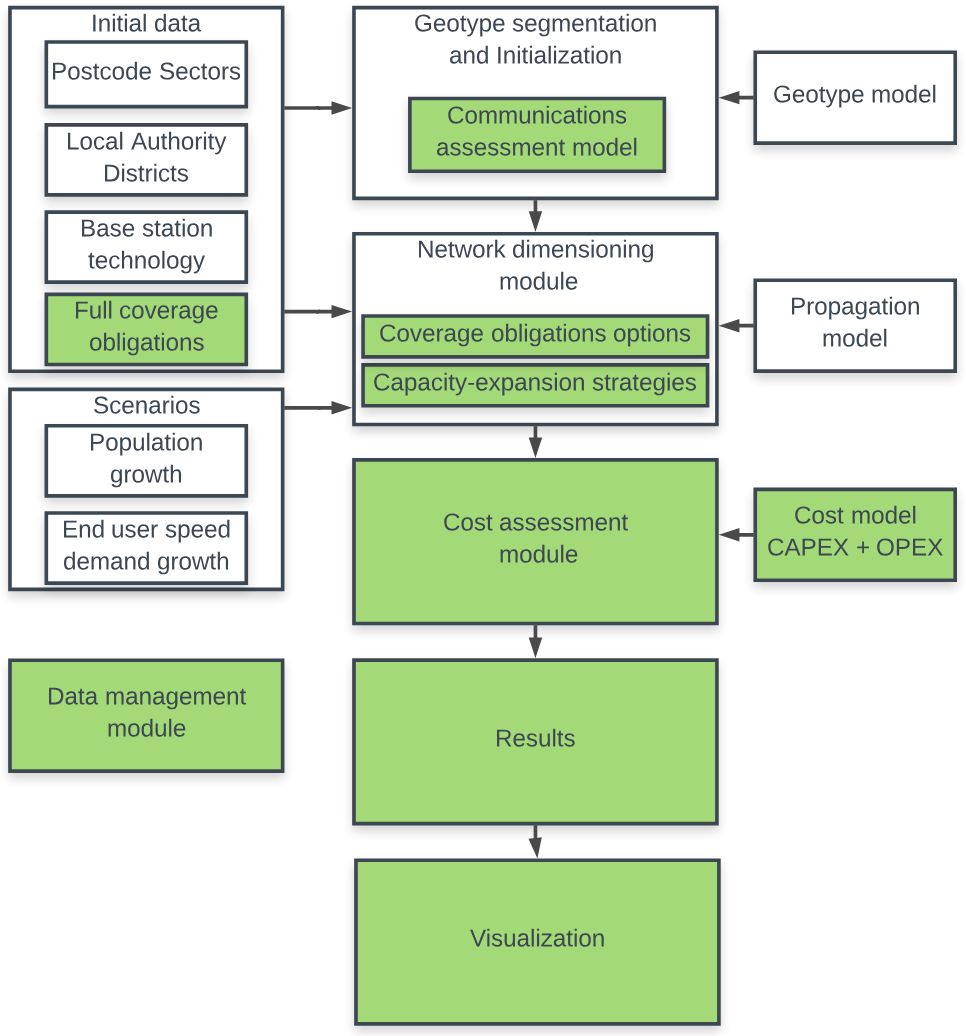
\includegraphics[width=0.95\textwidth]{./media/image28.png}
		\caption{NISMOD architecture with the new modules. Source: Author}
	\end{Center}
\end{figure}


%%%%%%%%%%%%%%%%%%%% Figure/Image No: 28 Ends here %%%%%%%%%%%%%%%%%%%%

\subsection{Coverage obligations options}
%\addcontentsline{toc}{subsection}{Coverage obligations options}
This project is aimed at defining realistic coverage obligations to test real scenarios. Coverage obligation options defined in this chapter base on the analysis presented in chapter 2 where we reviewed the content and characteristics of coverage obligations in some of the countries in Europe. The analysis was mainly focused on Spain, the UK, France, and Germany. \par

The characteristics of these coverage obligations have been extracted and condensed in the following four options: \par

\begin{itemize}
	\item \textit{«Priority areas first»} forces telecom operators to invest only in rural areas.\par

	\item \textit{«Less profitable first»} forces to invest first in the most profitable areas of each nation.\par

	\item \textit{«Only rural areas forces»} to invest in the priority areas first.\par

	\item \textit{«Nation-balanced»} forces to invest first in the less profitable areas. 
\end{itemize}\par

In addition, two more simple options have been defined to understand the rest: \textit{«Business as usual»} and \textit{«More profitable first».}\par

In this section, we define these options and how they operate. Later on, in chapter 4, we will analyze how they work in the simulation and which advantages and disadvantages they have.\par

\subsubsection*{Business as usual (No coverage obligations)}
%\addcontentsline{toc}{subsubsection}{Business as usual (No coverage obligations)}
This is, strictly speaking, not a coverage obligation option since there are no coverage obligations here. The following diagram represents all the PCDs in descending order from higher population density to lower density. As, in this case, telecom operators do not have to invest imperatively in any area, they would logically build assets first in those areas that demand more capacity than what is installed starting in those regions were investing is more profitable than others. In the diagram, the full line is red coloured because no PCD will receive more or fewer investments due to coverage obligations.



%%%%%%%%%%%%%%%%%%%% Figure/Image No: 29 starts here %%%%%%%%%%%%%%%%%%%%

\begin{figure}[H]
	\begin{Center}
		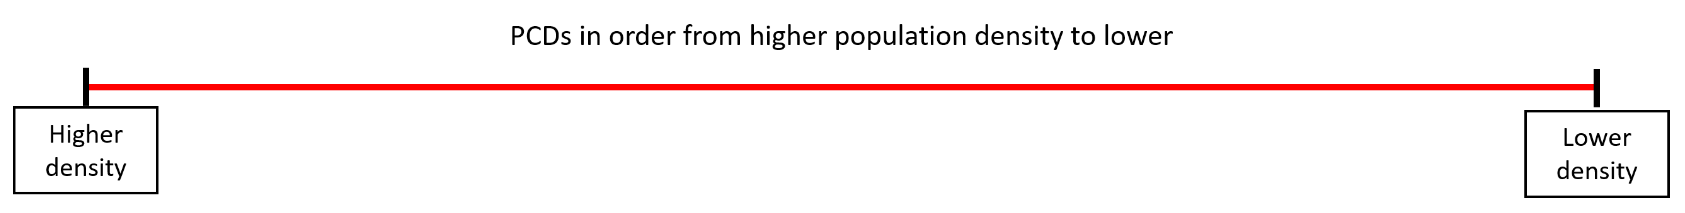
\includegraphics[width=0.95\textwidth]{./media/image29.png}
		\caption{Coverage obligations in \textit{«Business as usual»}. Source: Author}
	\end{Center}
\end{figure}


%%%%%%%%%%%%%%%%%%%% Figure/Image No: 29 Ends here %%%%%%%%%%%%%%%%%%%%


\subsubsection*{More profitable first (Original model)}
%\addcontentsline{toc}{subsubsection}{More profitable first (Original model)}
This other option is just the simple model that does have a coverage obligation, but where there is no coverage obligation compliance. This way, the telecom operator will be forced to achieve a minimum user download speed for a given year, but it will not need to do it in a specific way, technology, or band, and neither to invest in some specific areas before others. This is the behaviour of the original NISMOD project and will be used as a template to compare with the rest of them.\par

The following diagram represents the way telecom operators would probably invest if they follow this option. They would like to maximize profitability and thus, in a similar way as in the business as usual case, they would start to invest in the most densely populated PCDs until they can cover the coverage obligations in this PCD. Then they will continue investing until they reach a certain percentage of the population covered, where they will stop.



%%%%%%%%%%%%%%%%%%%% Figure/Image No: 30 starts here %%%%%%%%%%%%%%%%%%%%

\begin{figure}[H]
	\begin{Center}
		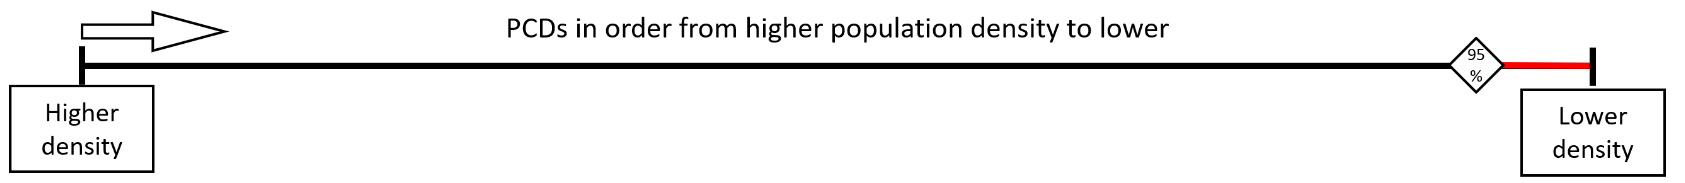
\includegraphics[width=0.95\textwidth]{./media/image30.png}
		\caption{Coverage obligations in \textit{«More profitable first»}. Source: Author}
	\end{Center}
\end{figure}


%%%%%%%%%%%%%%%%%%%% Figure/Image No: 30 Ends here %%%%%%%%%%%%%%%%%%%%


Note that the red line represents the part of the PCDs that will be left out of the coverage obligations.\par

\subsubsection*{Priority areas first (France)}
%\addcontentsline{toc}{subsubsection}{Priority areas first (France)}
This option is inspired by the coverage obligations that Arcep, the French regulator, imposed on telecom operators in France. This option tests the efficiency and the profitability of creating a priority area where telecom operators must invest first to be allowed to follow to cover the same (or a different) coverage obligation in the rest of the PCDs.\par

This thesis uses the UK’s geographic and demographic data to test all the coverage obligations in a similar scenario, so there is no list of the priority areas of the UK. As selecting the areas that are less developed in telecommunication services in the UK would not imply to have better results, the approach followed in the thesis is to select areas that sum the same population in the UK than the priority areas from France, which were 18$\%$  of the population according to Arcep. Those PCDs will be chosen beginning at the most rural PCD.\par

Once the limit is established, if telecom operators would like to maximize their profitability, they would roll out broadband services in three steps:\par

	\item Invest first starting in the limit $``$priority – non-priority$"$  covering the priority areas.\par

	\item Then, start in the most profitable PCD and continue until every PCD has their coverage obligations fulfilled.\par

	\item After that, they would be able to build more assets to increase the capacity of those PCDs that still need more investment.\par

The following diagram shows this option and allows to compare it with the previous ones. Note that in this option no minimum percentage has been defined so every postcode has to fulfil the obligations. This is completely customizable in the code, but the decision has been taken because Arcep defined a 99.6$\%$  coverage obligation in the entire territory and this option wants to check the effects that this decision will have in the costs.



%%%%%%%%%%%%%%%%%%%% Figure/Image No: 31 starts here %%%%%%%%%%%%%%%%%%%%

\begin{figure}[H]
	\begin{Center}
		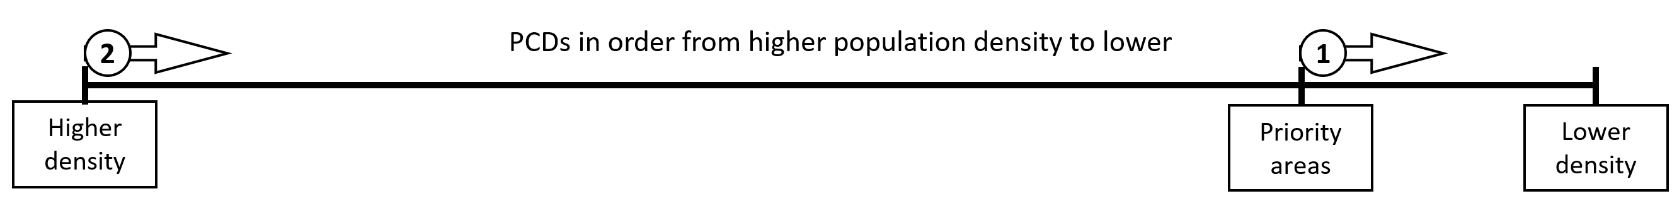
\includegraphics[width=0.95\textwidth]{./media/image31.png}
		\caption{Coverage obligations in \textit{«Priority areas first»}. Source: Author}
	\end{Center}
\end{figure}


%%%%%%%%%%%%%%%%%%%% Figure/Image No: 31 Ends here %%%%%%%%%%%%%%%%%%%%


\subsubsection*{Less profitable first (Germany)}
%\addcontentsline{toc}{subsubsection}{Less profitable first (Germany)}
This option is based on the strategy that Germany followed to set their coverage obligations. They defined four groups according to population density and only allowed telecom operators to invest in more densely populated groups if they had achieved a minimum percentage of coverage in the lower ones. This strategy is interesting because investments are not motivated by a necessity of fulfilling obligations but by their interest in investing as soon as possible in the most profitable areas.\par

For the sake of simplicity, no intermediate steps have been defined, just a global 95$\%$  of the population covered by the obligations at the end of the period. In this scenario, the normal approach of each telecom operator would be to not consider the 5$\%$  less profitable part of the population.\par

Once the 95$\%$  of the population is selected, according to this option, the telecom operator will invest in the less profitable areas and then it will continue area per area, investing in all the areas that need to improve their assets to meet the coverage obligations until they finish building assets in the most profitable one. The following diagram shows how a telecom operator should invest in the $``$Less profitable first$"$  scenario:



%%%%%%%%%%%%%%%%%%%% Figure/Image No: 32 starts here %%%%%%%%%%%%%%%%%%%%

\begin{figure}[H]
	\begin{Center}
		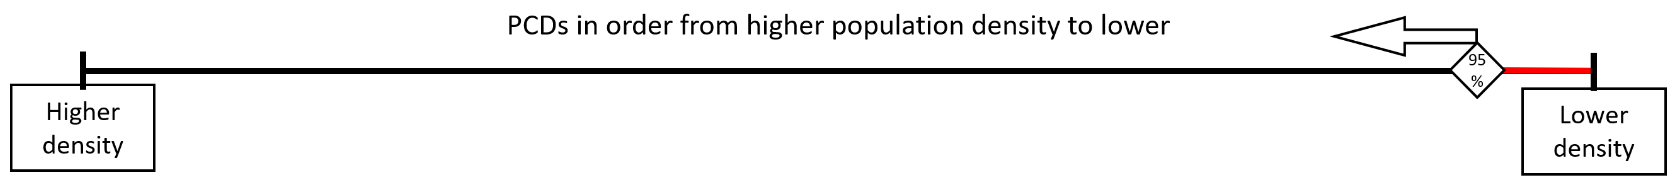
\includegraphics[width=0.95\textwidth]{./media/image32.png}
		\caption{Coverage obligations in \textit{«Less profitable first»}. Source: Author}
	\end{Center}
\end{figure}


%%%%%%%%%%%%%%%%%%%% Figure/Image No: 32 Ends here %%%%%%%%%%%%%%%%%%%%



Note that the red line represents the part of the PCDs that will not be affected by the coverage obligations.\par

\subsubsection*{Only rural areas (Spain)}
%\addcontentsline{toc}{subsubsection}{Only rural areas (Spain)}
The following option is focused on only balancing the mobile broadband gap that occurs in most of the countries between the rural and the urban and suburban areas. This option is based on the coverage obligations that Spain established for telecom operators in Spain. The interesting point of this option is that it does not enforce a coverage obligation for most of the regions, but only for those that are less populated.\par

This strategy first looks for those regions that are rural, due to their population. These are the only regions that are affected by the coverage obligation. After that, the obligation says that with only 90$\%$  of those is enough to fulfil the obligation, so following the same approach of before, it is expected that the 10$\%$  of the rural PCDs that is less populated will be excluded.\par

Of course, after fulfilling the coverage obligations, telecom operators can invest in any PCD to improve the capacity of the network and provide more download speed to their users, but this is not part of the coverage obligation.



%%%%%%%%%%%%%%%%%%%% Figure/Image No: 33 starts here %%%%%%%%%%%%%%%%%%%%

\begin{figure}[H]
	\begin{Center}
		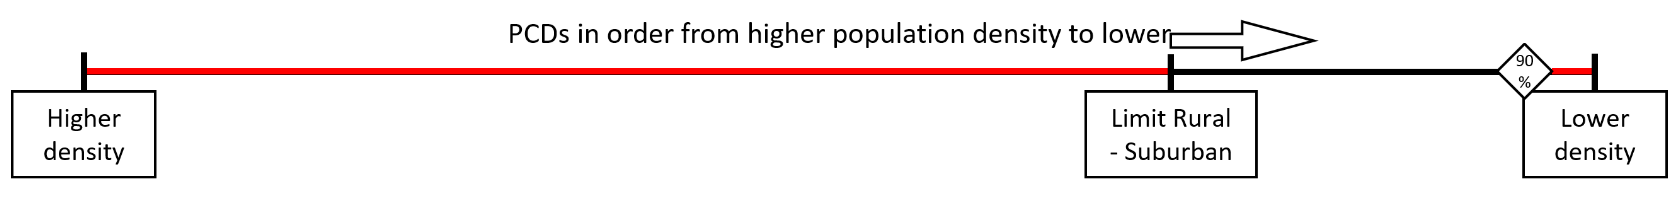
\includegraphics[width=0.95\textwidth]{./media/image33.png}
		\caption{Coverage obligations in \textit{«Only rural areas»}. Source: Author}
	\end{Center}
\end{figure}


%%%%%%%%%%%%%%%%%%%% Figure/Image No: 33 Ends here %%%%%%%%%%%%%%%%%%%%


\subsubsection*{Nation-balanced (The United Kingdom)}
%\addcontentsline{toc}{subsubsection}{Nation-balanced (The United Kingdom)}
This is the last option proposed in this project and is related to the coverage obligation imposed in the UK. The UK comprises four nations with different characteristics in the telecommunications field. First, England is by far the most populated and also contains most of the densely populated areas. On the contrary, regions like Scotland are more rural, have more uninhabited areas and more mountainous terrain, which make most of their PCDs less profitable to invest in. For that reason, Ofcom, the British policymaker, decided to split the coverage obligations into the four countries, so that telecom operators invest in all the countries equally independently of the profitability of investing more in some than in others.\par

This option is like the $``$More profitable first$"$  option but split into countries. The algorithm still checks all the PCDs in order from more profitable to less but keeps the percentage of people that are covered in each country. When one country is completely covered, the algorithm continues checking but no more PCDs from this country can be considered.



%%%%%%%%%%%%%%%%%%%% Figure/Image No: 34 starts here %%%%%%%%%%%%%%%%%%%%

\begin{figure}[H]
	\begin{Center}
		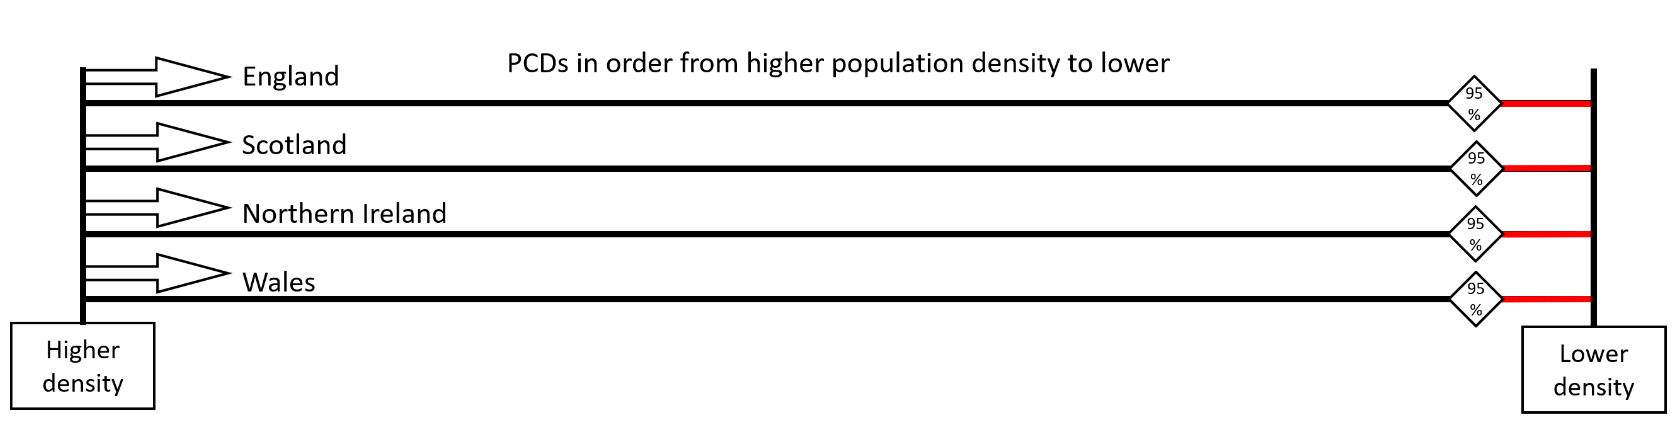
\includegraphics[width=0.95\textwidth]{./media/image34.png}
		\caption{Coverage obligations in \textit{«Nation-balanced»}. Source: Author}
	\end{Center}
\end{figure}


%%%%%%%%%%%%%%%%%%%% Figure/Image No: 34 Ends here %%%%%%%%%%%%%%%%%%%%

\subsection{Initial Data}
Two main improvements have been undertaken in this part of the code: the implementation of the Data Management Structure and the code to define coverage obligations. Nonetheless, other parts of the code have been modified and refined such as the new simulation options (To test new scenarios) and the new parameters of the end-user speed (Which is loaded from a file in this step).\par

\subsubsection*{Data management structure}
%\addcontentsline{toc}{subsubsection}{Data management structure}
The data management structure is a module called ‘\textit{results.py’} that is initialized at the beginning of the execution and stores all the information that the user might want to print at the end. It is just a class called Results that contains several sets of Chart subclasses for each simulation option. Chart subclasses are classes that store information of each PCD and are so related to each of the charts that are drawn from the execution. Some columns such as the PCD ID and the PCD population are initialized at the beginning and after that, each valuable output is picked and copied to the structure. When the Visualization module is called, it looks for all these classes, takes the information and manipulates it to print plots, maps and csv. \par

It also allows storing some environment values that will remain unchangeable during a great part of the execution of the code. It stores the output paths of the plots and maps modules, the total population of the country to reduce the time-consuming task that is to add the population of 9,000 PCDs every time the code needs to know the total population of the country, it stores the maps file paths of the images that will be added to gifs and it also stores all the information of the coverage obligation that is set at any time. \par

In the end, this module acts as a big bundle that allows having everything ready to use, saving time and resources.\par

\subsubsection*{Coverage obligations structure}
%\addcontentsline{toc}{subsubsection}{Coverage obligations structure}
In order to make coverage obligations completely customizable and adjustable, they are defined in a dictionary at the beginning of the execution and loaded into the Data management structure, so that the information about the current coverage obligation can be checked at any one moment.\par

These are the parameters that I have selected to describe a coverage obligation in this thesis: \par

\begin{enumerate}
	\item The coverage id, name, and description to have an unambiguous identifier of the obligation.\par

	\item The population limit, defined with a Boolean and a number limit, which defines the maximum population of the PCDs that are subject to the coverage obligations. \par

	\item The priority deployment that determines the percentage of the population whose PCDs will be part of the priority deployment areas. In this case, only France will have a number different from 0, but any coverage option could implement this strategy.\par

	\item The budget limits Boolean defines if this coverage obligation option is limited by the budget estimated for each telecom operator or not. The estimated budget amounts to 2 billion pounds multiplied by the market share (30$\%$  in this case) per year. This option will be used in the results chapter to check how much money would be necessary to fulfil the coverage obligations in case that not everybody can be covered with the estimated budget.\par

	\item The descending order parameter defines if the telecom operator should start investing in the more or the less profitable areas first. This Boolean is always true, except in the $``$Less profitable first$"$  option, where it is false, which inverts the order of investment decision of the PCDs.\par

	\item Invest by demand is a parameter that allows setting if, after investing to meet the coverage obligations, the telecom operator can continue investing money to build assets that can increase the capacity of the network to meet the demand in those PCDs where it is higher than the coverage obligations.\par

	\item The percentage covered is the minimum percentage of the population that the policymaker requires the telecom operators to cover. It depends on the coverage obligation and in the case of the $``$Only rural areas$"$  option, the percentage applies only to the rural areas, not to the total of PCDs.\par

	\item Finally, coverage\_obligation is a sub-dictionary that allows setting several end-user speeds depending on the requirements of the policymaker. There are three possible levels: Low, baseline and high and in this example the values are 2, 5 and 8 Mbps.
\end{enumerate}
\begin{lstlisting}[language=Bash]
'cov_ob_1': {
        'name': 'Coverage Obligation 1',
        'description': 'Original coverage obligation',
        'population_limit_boolean': False,
        'population_limit': None,
        'deploiement_prioritaire': 0,
        'budget_limit': True,
        'descending_order': True,
        'invest_by_demand': True,
        'percentage_covered': 1,
        'coverage_obligation': {
                'low': 2,
                'baseline': 5,
                'high': 8
        },
    }
\end{lstlisting}

\subsubsection*{Simulation options}
%\addcontentsline{toc}{subsubsection}{Simulation options}
Two new options have been added to the model to be able to test all the possibilities of the code and both are related to the coverage obligations:\par

	\item \textit{coverage\_obligation\_type} is the variable that specifies the option set for this execution of the code. It may take one of the values defined in the coverage obligations structure.\par

	\item \textit{coverage\_speed\_scenario }is the degree of intensity of the coverage obligation set by the policymaker. \par

\subsection{Geotype segmentation and initialization}
The only change in this module is in the way the code sorts each PCD into geotypes.\par

\subsubsection*{Change of rural-suburban-urban}
%\addcontentsline{toc}{subsubsection}{Change of rural-suburban-urban}
The function that categorized the code in the previous code had a bug that only set as rural areas those with 0 or less population density and urban areas from 782 inhabitants per km\textsuperscript{2}. This thesis raises the population ranges and categorizes areas from 0 to 782 inhabitants per km\textsuperscript{2} as rural, from 782 to 7,959 inhabitants per km\textsuperscript{2} as suburban and from 7,959 inhabitants on as urban.\par

After making those changes, an issue arises since some PCDs that are now categorized as rural, but have a high population density (For example, 600 inhabitants per km\textsuperscript{2}) cannot satisfy the demand. This is because the propagation diagrams estimate less network capacity for rural areas than for suburban geotypes. It is not a problem or a bug by itself, it just modifies considerably the predictions made based on the previous behaviour of the project.\par

\subsection{Scenario projections}
Changing the population and end-user projection is out of the scope of the thesis because this is part of the NISMOD project and not of the digital comms submodule, but this Thesis presents an enhancement of the end-user speed demand calculation.\par

\subsubsection*{Demand in Speed or Download cap}
%\addcontentsline{toc}{subsubsection}{Demand in Speed or Download cap}
The original project calculates the end-user speed demand in downloaded GB per month and then transforms this real measured demand to Mbps multiplying it by 1024 MB in 1 GB, 8 bits in a byte, 30 days in a month, percentage\_in\_busy\_hour (which is 7.5$\%$  of the traffic of the day) and 3600 to convert from hours to seconds.\par


\begin{Center}
\begin{multline*}
Demand \_ in \_ mbps =Demand \_ in \_ GB \ \ast \ 1024 \ \ast 8 \ast \\
 Traffic \_ in \_ busy \_ hour \ / 30 \ / 3600
\end{multline}
\end{Center}\par

The problem in this estimation is that user satisfaction is not only based in the amount of data the user can download during the day but in the maximum peak speed, the user can obtain from the network. Users will have a better user-experience if both demands are covered.\par

For this purpose, the code has been modified to implement both comparisons and the demand is the more restrictive value from the demand by speed and demand by download capacity.\par

In the newest version of the code, the user can create a csv file to introduce the evolution of the user demand in Mbps for each year until 2030 for three different scenarios: low demand, baseline demand, and high.\par

\subsection{Network dimensioning module}
This is the module that suffered more technical changes since now the model behaves quite different as it does at the beginning of the thesis. There are two big changes in this module: \par

\begin{itemize}
	\item The implementation of a new strategy called 700 MHz densification, that allows creating more assets for 700 MHz when the existing ones are already upgraded to 700 MHz until the maximum capacity of the network is reached (The maximum capacity is calculated using the propagation model).\par

	\item The creation of a more complex way of organizing the PCDs to comply with the obligations.
\end{itemize}\par

This module consists of several steps that enable to decide the interventions of all the PCDs for the whole year:\par

\begin{enumerate}
	\item Once a new year starts, this module is called to select those PCDs that, according to the coverage obligation option should meet the obligations, and orders them according to the option.\par

	\item It removes from the list those PCDs that already met the coverage obligation, thanks to the assets that were already installed before the execution or because they were built in a previous year in the simulation.\par

	\item For each PCD, it checks which are the interventions that are allowed according to the capacity expansion strategy and builds new assets in a given order. If all the interventions are allowed, the order is the following:\par

\setlength{\parskip}{7.92pt}
\begin{enumerate}
	\item First, it checks if more LTE upgrades are possible.\par

	\item If the capacity is not enough, it also integrates the 700 MHz band (This integration can be just upgrading the current assets or building new ones, it depends on the coverage obligation option).\par

	\item It integrates the 3,500 MHz band.\par

	\item The last resource is to build small cells.\par


\end{enumerate}
	\item This loop continues checking each PCD until there is no more budget for the given year or when the full list of PCD meets the coverage obligations and there is more budget.\par

	\item {\fontsize{11pt}{13.2pt}\selectfont In case that there is no more budget, the execution ends. In the other case, the code lists all the PCDs from more densely populated to less, removes those whose capacity margin is positive (Because they do not need more investment) and repeats the previous steps but with this list until there is no more budget.\par}
\end{enumerate}\par

Finally, all the new assets are stored and loaded into the system model to use them in the following year.\par

\setlength{\parskip}{8.04pt}
\subsubsection*{Coverage obligations}
%\addcontentsline{toc}{subsubsection}{Coverage obligations}
As seen, the network dimensioning module has four steps: select PCDs for the coverage obligations, invest, select all the PCDs that have a capacity deficit and invest to increase their network capacity.\par

The code modification needed for the coverage obligations feature modifies the first step. Based on the coverage obligation id and parameters, the code selects and orders PCDs in a specific way. The code also orders the visualization module PCDs in the same way, so they are displayed correctly. \par

\subsubsection*{700MHz Densification}
%\addcontentsline{toc}{subsubsection}{700MHz Densification}
The 700 MHz densification is the new intervention designed in the thesis and it is implemented in this module. In this work, it only belongs to the macrocell\_only\_700 capacity expansion strategy which only allows the 700 MHz densification intervention when it is enabled, but it is configurable in the initialization structures.\par

As 700 MHz could be built using the already installed assets or standalone installations, this intervention functions as a combination of the behaviour of the normal 700 MHz and the small cells interventions. When the network dimensioning module selects one PCD to invest and this intervention is triggered, it checks how many assets have LTE and 700 MHz carriers. If there are assets that still have no 700 MHz carrier but have the LTE bands available, the intervention just builds a new 700 MHz carrier on the asset. If there are no more assets without 700, it deploys a new base station with 700 MHz. Costs of both scenarios are different and calculated based on the costings tables.\par

\subsection{Cost assessment module}
Costs are calculated in the same way as in the original model. After the execution of all the interventions, the full list of new assets is checked by the cost assessment module and the total cost of the year is calculated.\par

\subsubsection*{Cost model}
%\addcontentsline{toc}{subsubsection}{Cost model}
The cost model has been updated to include the new intervention costs. In case of building a new carrier in an existing installation, the cost is the same as in the 700MHz intervention: CAPEX is the cost of installing an additional carrier on the current base station, which is £15,000, and OPEX is £1,800. Therefore, the total cost discounted to the present value is £50,917.\par

For new installations, costs are like deploying a new base station for LTE, despite 700MHz would be the only carrier available. In this case, CAPEX is the cost of deploying two multicarrier base stations (2 x £40,900) plus the cost of the civil works (£18,000) and OPEX is £3,898 per year. The total cost discounted to the present value is £142,446. For a deeper explanation of costs, please refer to the Cost assessment module section of the original project or \cite{3-03}.\par

\subsection{Model results}
While deciding the interventions and calculating costs, the program stores and computes some key values of the system, so that the visualization model can store it later. Apart from storing values of costs and capacity margin, which was already implemented and explained in the previous chapter, it calculates (I) the percentage of population in each PCD that has the minimum capacity that the coverage obligation defines, (II) the number of assets that are upgraded or built depending on the technology per PCD, (III) values of population, (IV) demand and capacity per PCD and (V) global values calculated after deciding all the interventions of a simulation.\par

It is also capable of aggregating all of this data to the LAD level. Some values can be added directly, such as population and costs, but others, such as the percentage of population covered or the capacity margin not. Therefore, these parameters are aggregated weighted by population.\par

All the values are stored in the Results module, which is initialized in the $``$Initial Data$"$  step and then the rest of parameters are added whenever they are available. The results module is just a class that contains several dictionaries of classes that store all the values. Each set is different since they contain different types of subclasses, each of them defined to store information of one specific value. This way, despite some information, could be stored redundantly, it allows to expand the capabilities faster because creating a new table calculating new values means simply creating a new set and previous information is not altered.\par

\subsubsection*{Population, demand, and capacity}
%\addcontentsline{toc}{subsubsection}{Population, demand, and capacity}
In previous versions of the code, these were intermediate values to decide interventions and to calculate demand and capacity, but their evolution was not stored. Now, the visualization module shows the change of them over time and generates plots, maps, and csv with their values. The following map, for example, shows the population per PCD at the beginning of the execution, in 2020. It can be visualised over the entire period under study.



%%%%%%%%%%%%%%%%%%%% Figure/Image No: 35 starts here %%%%%%%%%%%%%%%%%%%%

\begin{figure}[H]
	\begin{Center}
		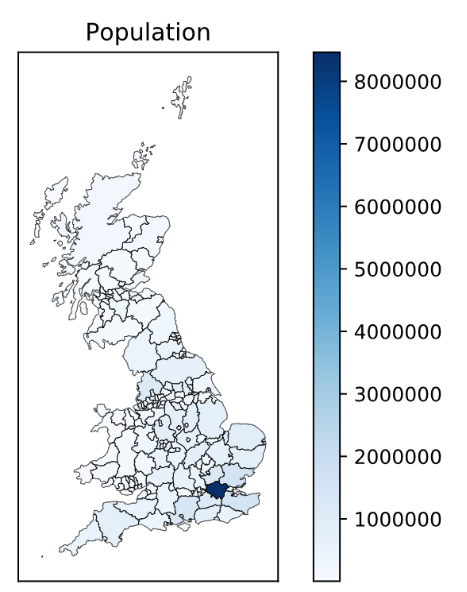
\includegraphics[width=0.70\textwidth]{./media/image35.png}
		\caption{Population distribution in the UK. Source: Author}
	\end{Center}
\end{figure}


%%%%%%%%%%%%%%%%%%%% Figure/Image No: 35 Ends here %%%%%%%%%%%%%%%%%%%%



\subsubsection*{Technology upgrades}
%\addcontentsline{toc}{subsubsection}{Technology upgrades}
A similar situation occurs with the number of sites built or upgraded per technology per year. The code now stores all the information about technology upgrades and calculates the number of upgrades that occurred per year in each PCD. The visualization module outputs maps, csv files and figures with the evolution.\par

For example, the following coloured map represents the number of technology upgrades made in the execution of the scenario of medium growth of population and user-speed demand, with the $``$More profitable first$"$  coverage obligation option that enforces 2 Mbps and with the capacity expansion strategy that only allows building 700 MHz cells:



%%%%%%%%%%%%%%%%%%%% Figure/Image No: 36 starts here %%%%%%%%%%%%%%%%%%%%

\begin{figure}[H]
	\begin{Center}
		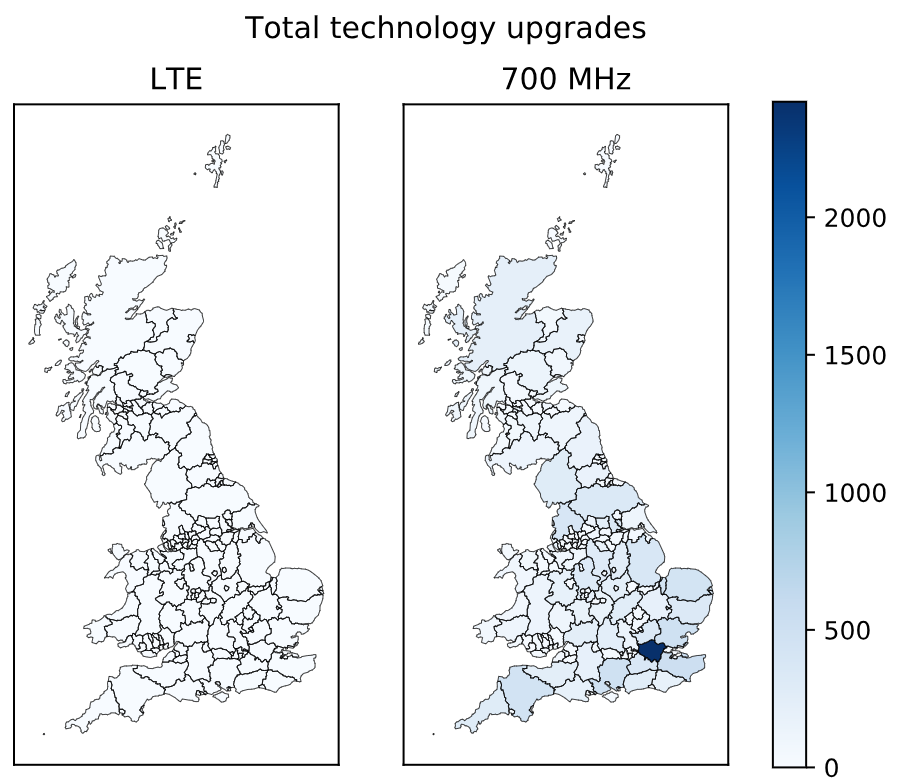
\includegraphics[width=0.85\textwidth]{./media/image36.png}
		\caption{Technology upgrades with \textit{«700MHz densification}. Source: Author}
	\end{Center}
\end{figure}


%%%%%%%%%%%%%%%%%%%% Figure/Image No: 36 Ends here %%%%%%%%%%%%%%%%%%%%


\subsubsection*{Population covered}
%\addcontentsline{toc}{subsubsection}{Population covered}
Population covered is another output of the project. When a year ends, the system computes the percentage of the population covered as the result of the division of the capacity by the download speed demand in each PCD. The result is capped to one since the population covered cannot be more than 100$\%$ .\par

The following coloured maps represent the population covered per year in the execution of the scenario of medium growth of population and user-speed demand, with the $``$More profitable first$"$  coverage obligation option that enforces 2 Mbps and with the capacity expansion strategy that only allows building 700 MHz cells:



%%%%%%%%%%%%%%%%%%%% Figure/Image No: 37 starts here %%%%%%%%%%%%%%%%%%%%

\begin{figure}[H]
	\begin{Center}
		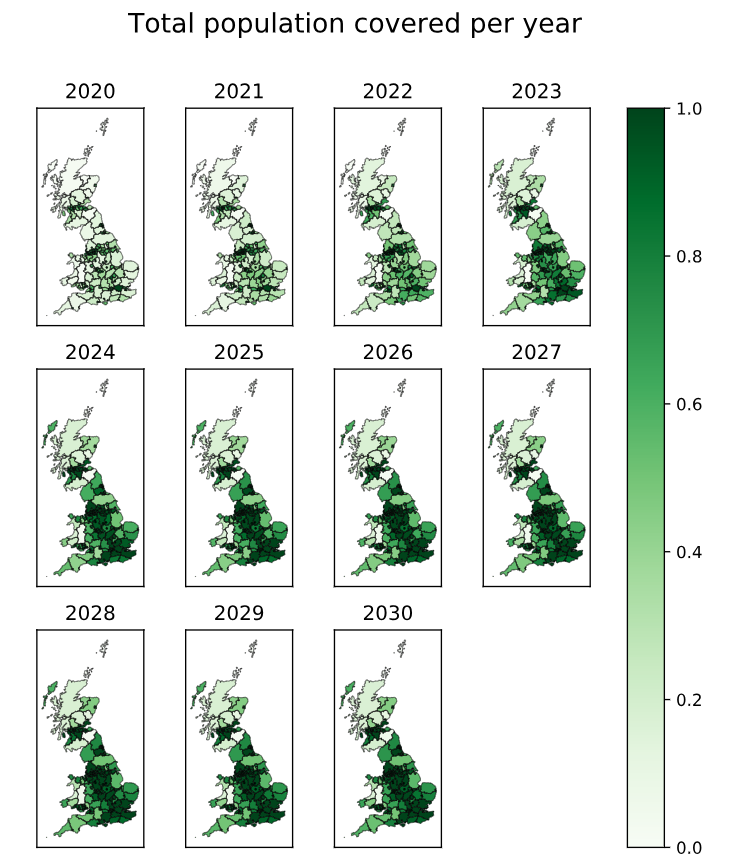
\includegraphics[width=0.95\textwidth]{./media/image37.png}
		\caption{Example of the evolution of the percentage of population covered with the \textit{«700MHz densification} capacity expansion strategy. Source: Author}
	\end{Center}
\end{figure}


%%%%%%%%%%%%%%%%%%%% Figure/Image No: 37 Ends here %%%%%%%%%%%%%%%%%%%%


\subsubsection*{How to aggregate capacity and demand values}
%\addcontentsline{toc}{subsubsection}{How to aggregate capacity and demand values}
Aggregating values from PCDs to LADs is not always as simple as just adding values. Aggregating costs and technology upgrades can be made just by adding values of each PCD. However, percentages of the population covered cannot be aggregated but weighted according to a specific factor, such as population or area. Since covered obligations are defined based on population, these values are weighted by population. \par


 \[ \% Population_{LAD}=\frac{ \sum _{1}^{N}Population_{PCD-i}  \times  \% Population_{PCD-i}}{ \sum _{1}^{N}Population_{PCD-i} } \] \par
	
	where N is the number of PCDs.

The capacity margin is expressed in Mbps/km\textsuperscript{2} and cannot be aggregated directly because is a relative measure, not an absolute value of capacity margin. This way, it must be weighted, as well. The following chart represents a LAD that contains 9 PCDs. Since coverage obligations are population oriented, if PCD 1 has 90$\%$  of the population and the rest is distributed among the others, the capacity margin of the PCD 1 has to weight 90$\%$  of the total calculus of the capacity margin. The following formula is used.



%%%%%%%%%%%%%%%%%%%% Table No: 7 starts here %%%%%%%%%%%%%%%%%%%%

\begin{table}[H]
\begin{center}
\begin{tabular}{ |c|c|c| } 
\hline
{\cellcolor[HTML]{2F5496}\Centering 1} & 2 & 3 \\ 
\hline
4 & 5 & 6 \\ 
\hline
7 & 8 & 9 \\ 
\hline
\end{tabular}
\end{center}
\end{table}


%\begin{table}[H]
 			%\centering
%\begin{tabular}{p{0.1in}p{0.1in}p{0.1in}}
%\hline
%%row no:1
%\multicolumn{1}{|p{0.1in}}{\cellcolor[HTML]{2F5496}\Centering 1} & 
%\multicolumn{1}{|p{0.1in}}{\cellcolor[HTML]{D9E2F3}\Centering 2} & 
%\multicolumn{1}{|p{0.1in}|}{\cellcolor[HTML]{D9E2F3}\Centering 3} \\
%\hhline{---}
%%row no:2
%\multicolumn{1}{|p{0.1in}}{\cellcolor[HTML]{D9E2F3}\Centering 4} & 
%\multicolumn{1}{|p{0.1in}}{\cellcolor[HTML]{D9E2F3}\Centering 5} & 
%\multicolumn{1}{|p{0.1in}|}{\cellcolor[HTML]{D9E2F3}\Centering 6} \\
%\hhline{---}
%%row no:3
%\multicolumn{1}{|p{0.1in}}{\cellcolor[HTML]{D9E2F3}\Centering 7} & 
%\multicolumn{1}{|p{0.1in}}{\cellcolor[HTML]{D9E2F3}\Centering 8} & 
%\multicolumn{1}{|p{0.1in}|}{\cellcolor[HTML]{D9E2F3}\Centering 9} \\
%\hhline{---}
%
%\end{tabular}
 %\end{table}


%%%%%%%%%%%%%%%%%%%% Table No: 7 ends here %%%%%%%%%%%%%%%%%%%%


 \[ Capacity\_ margin_{LAD}=\frac{ \sum _{1}^{N}Population_{PCD-i}  \times  Capacity\_ margin_{PCD-i}}{ \sum _{1}^{N}Population_{PCD-i} } \] \par
	
	where N is the number of PCDs.

\subsubsection*{Global variables}
%\addcontentsline{toc}{subsubsection}{Global variables}
Finally, some global values are also calculated after each simulation ends, and results of several simulations are compared to see the advantages or disadvantages of each of them. The values stored are the population, investment cost, population covered, number of PCDs covered and capacity margin per year. The array also stores if the model had enough budget to invest by demand.\par

The following diagram represents an example of the cost of incrementing the percentage of population covered for a given coverage obligation. The results and analysis section cover this in greater detail.



%%%%%%%%%%%%%%%%%%%% Figure/Image No: 38 starts here %%%%%%%%%%%%%%%%%%%%

\begin{figure}[H]
	\begin{Center}
		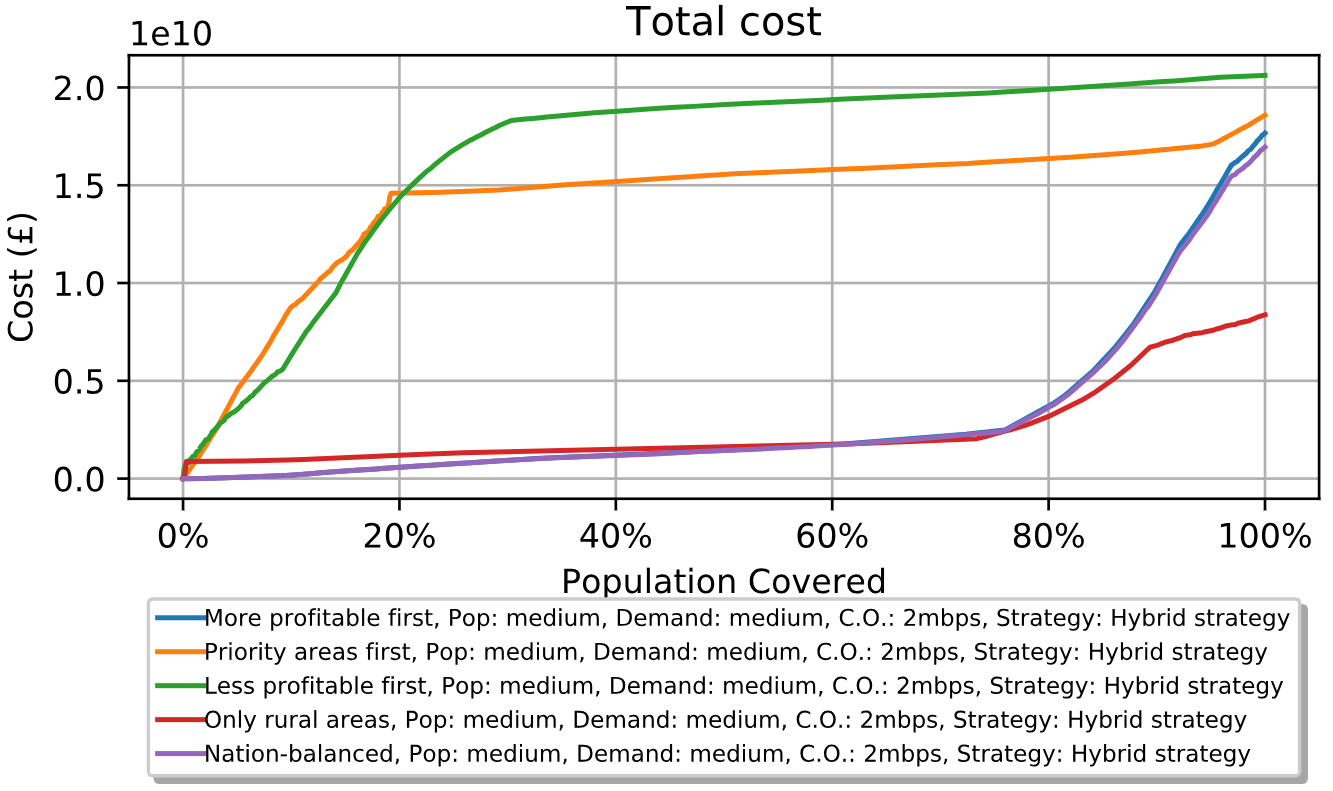
\includegraphics[width=0.95\textwidth]{./media/image38.png}
		\caption{Example of the investment with the \textit{«700MHz densification} capacity expansion strategy.Source: Author}
	\end{Center}
\end{figure}


%%%%%%%%%%%%%%%%%%%% Figure/Image No: 38 Ends here %%%%%%%%%%%%%%%%%%%%

\subsection{Visualization}
Once all the results are calculated and stored in the Results bundle, the code calls some functions of the Save Data module, which acts as a hub that takes the interesting results and represents them as csv, maps, plots, histograms or gifs. This functionality is completely new to the project and it is the tool that has been used to create all the diagrams and images of the results chapter.\par

\subsubsection*{Plots}
%\addcontentsline{toc}{subsubsection}{Plots}
Plots are the best way of comparing the output between different simulations of the project since they have more accuracy than maps (That do not have enough definition to see the differences between rural and urban areas), but they allow to see the whole picture of the situation (CSV files are so big that they are mainly used to check specific values). All the plots are allocated under the Outputs folder and inside the $``$figures$"$  folder. For a given simulation, the main plots drawn in the code are the following: \par

\begin{enumerate}[label*=\arabic*.]
	\item Aggregation of the investment in each PCD for all the years and calculation of the cost in pounds of increasing the population covered percentage. These plots start with the code 1\_1\_cost.\par

	\item Representation of the evolution of the investment through PCDs over the years. It allows seeing how the main part of the investment costs move from left to right, which means that the project invests in the same order of the list of PCDs, which depends on the coverage option. These plots start with the code 1\_2\_cost\_per\_year\_all.\par

	\item Representation of the technology upgrades through PCDs along the years. It allows seeing how the main part of the investment costs move from left to right, which means that the project invests in the same order of the list of PCDs, which depends on the coverage option. These plots start with the code 3\_1\_tech\_upgrades\_per\_year\_all.\par

	\item Representation of the capacity (Mbps per km\textsuperscript{2}) over the years in each PCD. These plots start with the code 4\_1\_capacity.\par

	\item Representation of the demand (Mbps per km\textsuperscript{2}) over the years in each PCD. These plots start with the code 4\_2\_demand.
\end{enumerate}\par

Despite all these representations study the implications of a single simulation, this module creates charts for comparing several of them, as well. There are three main plots:\par

\begin{enumerate}[label*=\arabic*.]
	\item Aggregation of the investment in each PCD for all the years and calculation of the cost in pounds of increasing the population covered percentage. This plot is under the summary folder and named \\
	1\_cost\_comparison\_per\_strategy.\par

	\item Comparison of the population covered per year and simulation option. This plot is under the summary folder and named \\
	2\_population\_covered\_per\_strategy.\par

	\item Comparison of the capacity margin per year and simulation option. This plot is under the summary folder and named \\
	3\_capacity\_margin\_per\_strategy.
\end{enumerate}\par

\subsubsection*{Histograms}
%\addcontentsline{toc}{subsubsection}{Histograms}
The main objective of the coverage obligations in most of the countries studied in chapter 2 is to reduce the end-user speed gap between the urban and the rural areas of the country. Studying the distribution of the capacity margin among all the PCDs allows the stakeholders to know the percentage of the population and the regions that have less capacity than the one enforced by the coverage obligation. The following chart shows an example of a histogram. In this case, the simulation represents the scenario of medium growth of population and user-speed demand, with the $``$Less profitable first$"$  coverage obligation option that enforces 2 Mbps and with the capacity expansion strategy that allows upgrading existing assets with LTE, 700MHz, 3,500 MHz and building small cells.



%%%%%%%%%%%%%%%%%%%% Figure/Image No: 39 starts here %%%%%%%%%%%%%%%%%%%%

\begin{figure}[H]
	\begin{Center}
		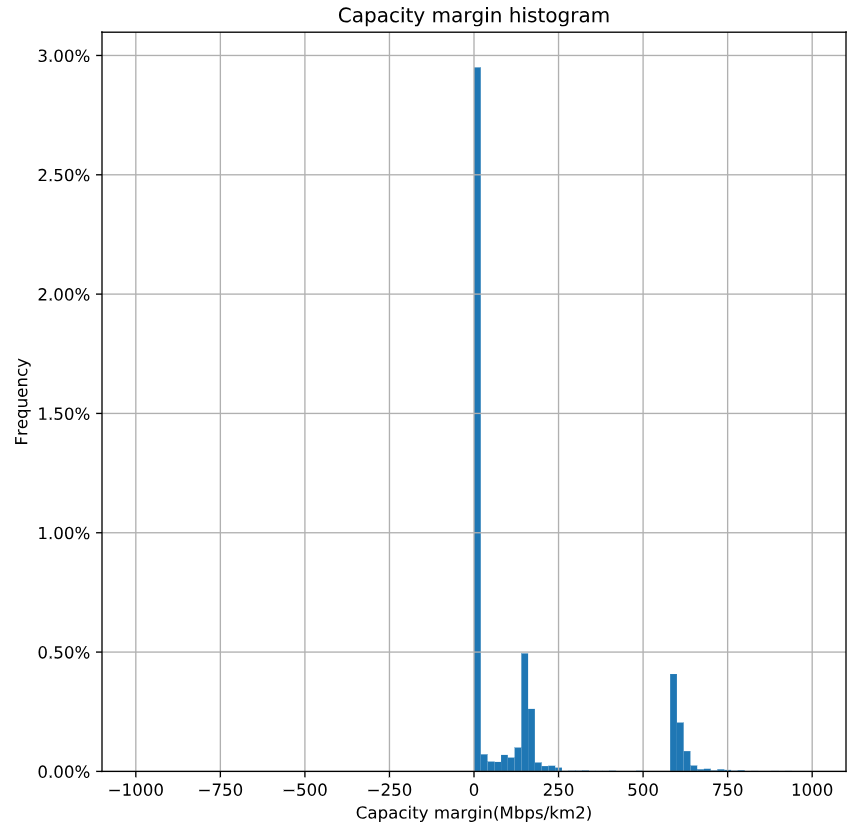
\includegraphics[width=0.95\textwidth]{./media/image39.png}
		\caption{Example of an histogram of the capacity margin per PCD with the \textit{«700MHz densification} capacity expansion strategy. Source: Author}
	\end{Center}
\end{figure}


%%%%%%%%%%%%%%%%%%%% Figure/Image No: 39 Ends here %%%%%%%%%%%%%%%%%%%%

\subsubsection*{Csv files}
%\addcontentsline{toc}{subsubsection}{Csv files}
Csv files store all the information related to the project. The advantage of this type of format is that they store the exact value of the outputs and allow to compare them with more detail than maps, plots or diagrams. There are two types of csv: Those that start with the code \textit{lad\_} refer to information represented in maps, the ones that start with the suffix \textit{pcd\_} contain information related to plots and histograms. \par

\subsubsection*{Maps}
%\addcontentsline{toc}{subsubsection}{Maps}
Maps represent outputs printed over the map of the UK and are drawn using the plot and fill functions of the matplotlib library. The UK shape is loaded from a shapefile stored in the inputs folder and can be replaced by the shape of other countries only if the PCDs and LADs are correctly modified. As it has been explained before, results have less level of detail since maps only have 174 regions. Several maps are painted automatically when the visualization module runs:\par

\begin{enumerate}
	\item Initial population and population density.\par

	\item Investment cost per LAD.\par

	\item Evolution of the cost per year.\par

	\item Evolution of the capacity margin per year.\par

	\item The number of technology upgrades per LAD.\par

	\item Evolution of the capacity per year.\par

	\item Evolution of the demand per year.\par

	\item Evolution of the population covered per year.
\end{enumerate}\par

Therefore, there are two main types of showing information in maps: standalone maps that aggregate outputs of all the years, and sprites of the situation every year.\par

\subsubsection*{Gifs}
%\addcontentsline{toc}{subsubsection}{Gifs}
Finally, the project also allows creating gifs from the images of the visualization model. The tool allows to create gifs of every value of the project, but it is focused in gifs that show the evolution of parameters such as the coverage obligation over the years, and to compare the differences between the coverage obligation resultant from different coverage obligation options and simulations.\par

\chapter{Analysis and results}
%\vspace{\baselineskip}
%\addcontentsline{toc}{section}{Analysis and results}
This chapter presents the results obtained from several simulations and compares them to analyse the differences across scenarios. The model allows to modify and customize several options, such as the population growth rate, the user-speed demand growth rate, the coverage obligations, the way this coverage obligations are enforced, and the capacity expansion strategies that the telecom operator can use to achieve the coverage obligation and meet the demand.\par

There are also some parameters of the code that are fixed a priori such as the overbooking factor of the macrocells, the percentage of traffic in the busy hour, if the operator invests only to meet the coverage obligation or to meet the demand, and if the operator has a limited budget or not. However, these can be modified to analyse the impact of variations of those parameters, too.\par

Regarding the PCDs and LADs, it is important to understand how they are distributed across the country. The following figures represent the population distribution, measured in aggregate population, and the population density distribution, measured in population per km\textsuperscript{2}. The values for each LAD are obtained at the beginning of the simulation (2020) and are equal for all the years. Despite these values vary over time depending on the population and end-user speed growth scenarios, this variation is homogeneous across the territory.\par



%%%%%%%%%%%%%%%%%%%% Figure/Image No: 1 starts here %%%%%%%%%%%%%%%%%%%%

\begin{figure}[H]
	\begin{Center}
		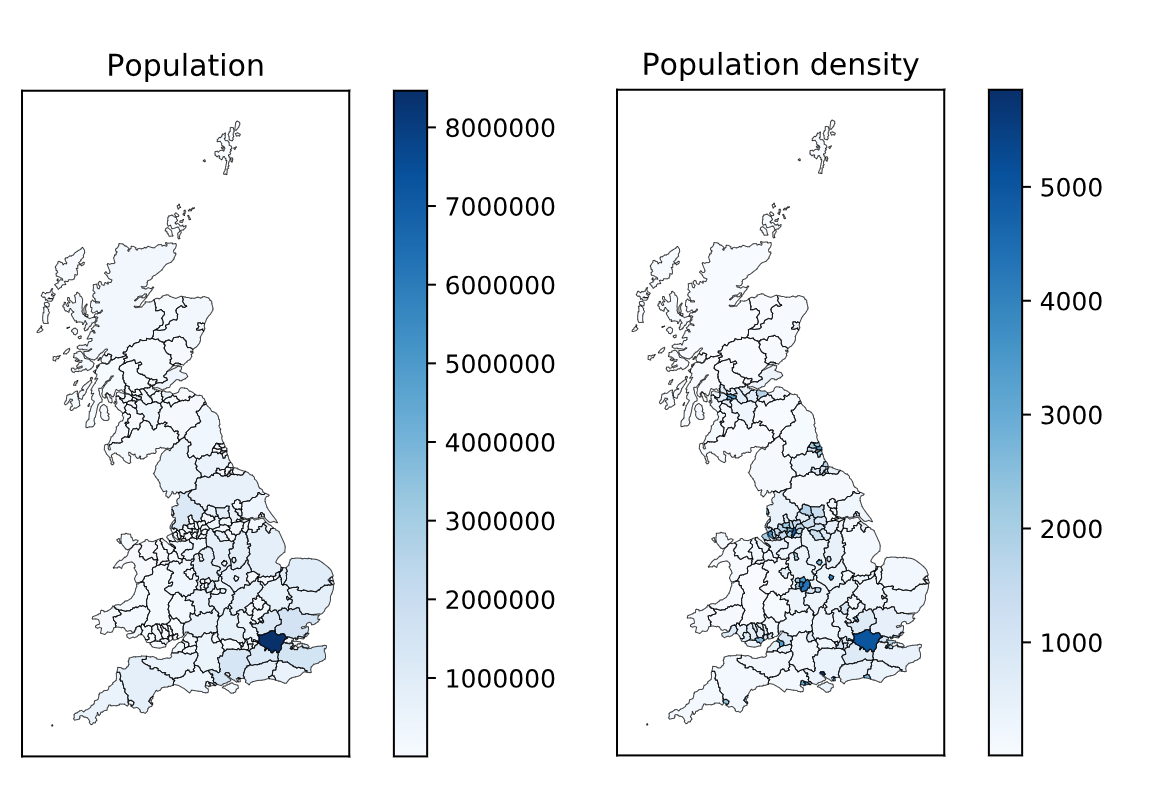
\includegraphics[width=0.95\textwidth]{./media/image40.png}
		\caption{Map. Population and population density. Source: Author}
	\end{Center}
\end{figure}


%%%%%%%%%%%%%%%%%%%% Figure/Image No: 1 Ends here %%%%%%%%%%%%%%%%%%%%

As it can be seen, the population is clearly higher in the London LAD, while the rest of the country have more similar population values (figure on the left). On the contrary, when we consider population density at the LAD, other regions in the UK become more important, matching with most of the important cities of the country: Manchester, Liverpool, Birmingham, Sheffield, Glasgow, etc. \par

In the following sections, I  present the simulations of different scenarios with different capacity expansion strategies and coverage obligation options. First, we evaluate the new capacity expansion strategy, 700 MHz densification. Then, we compare all the capacity expansion strategies and extract the key advantages and disadvantages of each of them. Finally, we test the coverage obligation options using two different strategies in the simulation to analyse how different coverage obligations affect the telecom operator in different ways depending on the strategy.\par


\section{700 MHz densification}
%\subsection*{700 MHz densification}
%\addcontentsline{toc}{subsection}{700 MHz densification}
700 MHz densification is the new intervention created in this Master Thesis. It consists in integrating the 700 MHz band in the existing base stations in the area and, once all of them have 700 MHz carriers, the intervention builds new base stations until the capacity demanded is reached, the coverage obligations are fulfilled, or the maximum site density is reached.\par

After that, I have created a new capacity expansion strategy, the �\textit{700 MHz densification�} that is only allowed to use the �\textit{700 MHz densification�} strategy.\textit{ }The following figures show the effects that using this capacity strategy has on the development of the mobile telecommunications network. \par

\subsection*{Investment}
%\addcontentsline{toc}{subsection}{Investment}
The cost distribution is the first of the two most important outputs to analyse of a simulation. The investment graph shows the evolution of the investment over the years and produces several important results: (i) It allows to check how much it has been spent per year, (ii) how many years the telecom operator exhausted all its budget, (iii) when the capacity cannot be further increased because it has reached the limit of the technology. \par

The following graph represents the investment made by the telecom operator per year to build new assets in all the country. The green line shows in which year the telecom operator starts to invest to satisfy the demand instead of investing to fulfil the coverage obligations. This test uses the baseline population growth scenario, the baseline user-speed growth scenario, and the \textit{�More profitable first�} coverage obligation option with a speed of 2 Mbps. \par



%%%%%%%%%%%%%%%%%%%% Figure/Image No: 2 starts here %%%%%%%%%%%%%%%%%%%%

\begin{figure}[H]
	\begin{Center}
		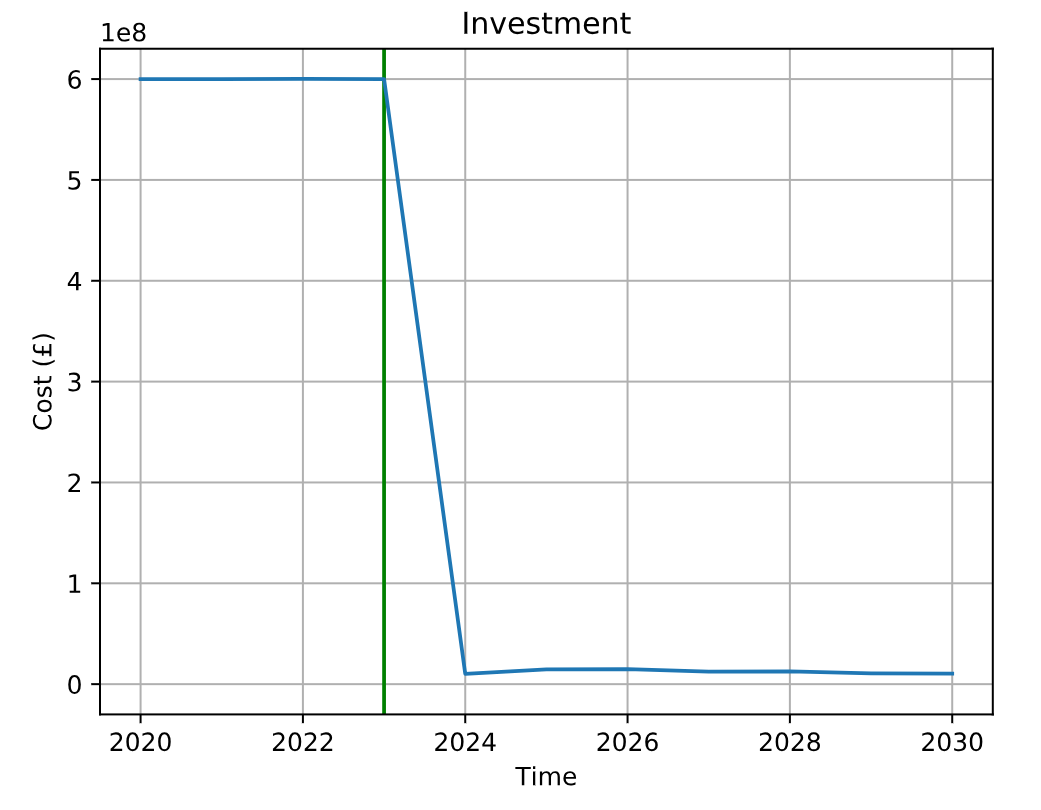
\includegraphics[width=0.85\textwidth]{./media/image41.png}
		\caption{700 MHz densification. Graph: Investment. Source: Author}
	\end{Center}
\end{figure}


%%%%%%%%%%%%%%%%%%%% Figure/Image No: 2 Ends here %%%%%%%%%%%%%%%%%%%%

As it can be seen, the investment is not the same every year. For the first 4 years (from 2020 to 2023) the telecom operator invests all the budget that it has: around �600,000,000. In the year 2023 the investment rate decreases to less than 10$\%$  of the maximum, two things could happen: (i) the telecom operator determines that is fulfilling the coverage obligations and stops investing, (ii) despite some regions still need more investment, it is not possible due to technical limitations. We need the population covered analysis to determine which is the case.\par

Another output that is important is the cost of increasing the population covered using this strategy. It is not linear since each geotype have different propagation characteristics. The following graph shows information related to this output:\par



%%%%%%%%%%%%%%%%%%%% Figure/Image No: 3 starts here %%%%%%%%%%%%%%%%%%%%

\begin{figure}[H]
	\begin{Center}
		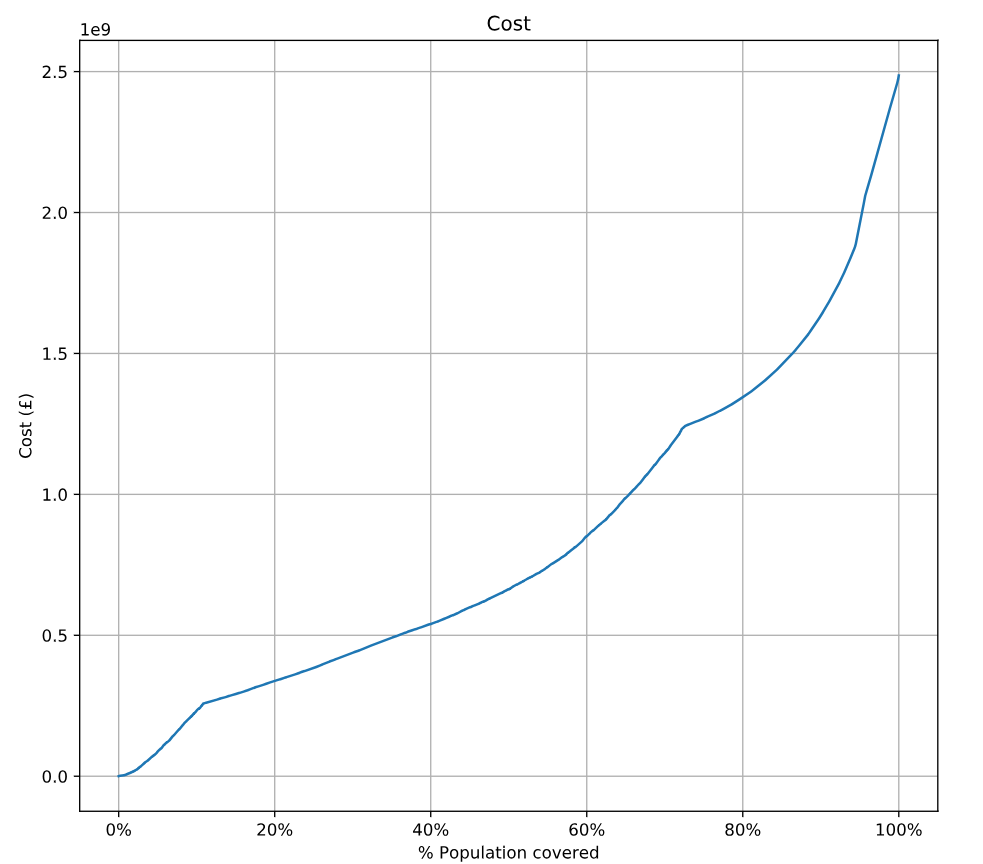
\includegraphics[width=0.95\textwidth]{./media/image42.png}
		\caption{700 MHz densification. Graph: Cost. Source: Author}
	\end{Center}
\end{figure}


%%%%%%%%%%%%%%%%%%%% Figure/Image No: 3 Ends here %%%%%%%%%%%%%%%%%%%%

This test uses the baseline population growth scenario, the baseline user-speed growth scenario, and the \textit{�More profitable first�} coverage obligation option with a speed of 2 Mbps. The graph represents the cumulative costs of having a certain percentage of population covered. It shows an increasing growth of the marginal costs as the coverage increases. The reason is that \textit{�More profitable first�} orders all the PCDs from most to least densely populated, which means that urban PCDs are first and rural PCDs are the last.\par

There are three main parts in which rates of cost increase could be divided: (i) Urban areas (circa 0$\%$  to 10$\%$ ), (ii) suburban areas (circa 10$\%$  to 75$\%$ ), and (iii) rural areas (circa 75$\%$  to 100$\%$ ). Despite the slope of the curve is not constant inside each part, in general terms, the slope is steeper for the rural areas because the population density is so low that the operator has to add ever more antennas. This is not because of capacity needs, but because of the limitation in range of coverage due to the attenuation losses. On the contrary, in highly populated areas, the operator is forced to build a lot of assets, because it needs a lot of capacity, but this strategy raises the costs significantly.\par

Finally, the following coloured map represents the distribution of costs across the country and how the most populated areas, especially London area, receive more investments during all the years:\par



%%%%%%%%%%%%%%%%%%%% Figure/Image No: 4 starts here %%%%%%%%%%%%%%%%%%%%

\begin{figure}[H]
	\begin{Center}
		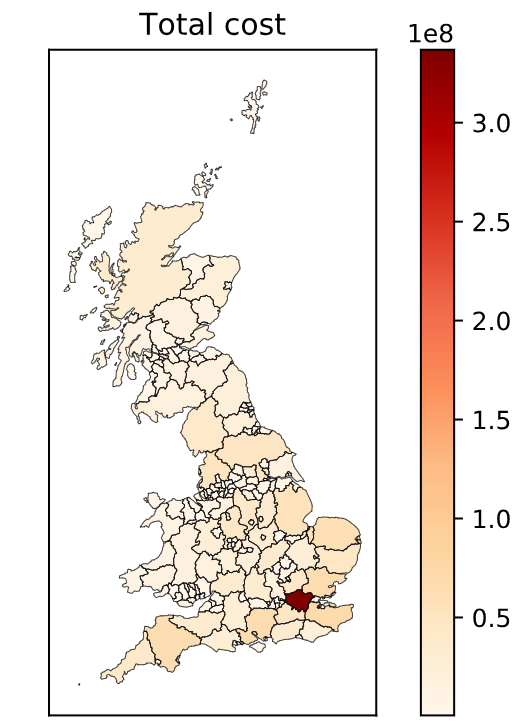
\includegraphics[width=0.65\textwidth]{./media/image43.png}
		\caption{700 MHz densification. Map: Total cost. Source: Author}
	\end{Center}
\end{figure}


%%%%%%%%%%%%%%%%%%%% Figure/Image No: 4 Ends here %%%%%%%%%%%%%%%%%%%%

\subsection*{Population covered}
%\addcontentsline{toc}{subsection}{Population covered}
The population covered over time is the second most important outputs to analyse. The detail per year produces three important results: (I) How the population is covered year by year, (II) If the given run is good enough to satisfy the demand and the coverage obligations in ten years, (III) If there are regions that simply cannot have enough capacity due to several reasons. The following map shows the evolution over time of the percentage of users that have at least the 2Mbps that the coverage obligation forces:\par



%%%%%%%%%%%%%%%%%%%% Figure/Image No: 5 starts here %%%%%%%%%%%%%%%%%%%%

\begin{figure}[H]
	\begin{Center}
		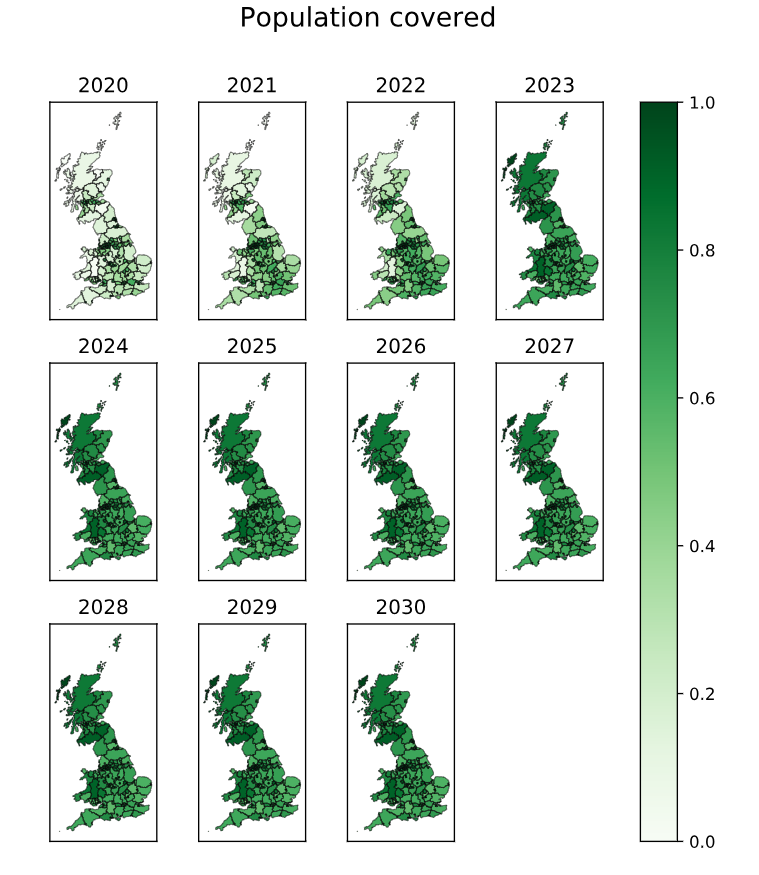
\includegraphics[width=0.95\textwidth]{./media/image44.png}
		\caption{700 MHz densification. Map: Population covered. Source: Author}
	\end{Center}
\end{figure}


%%%%%%%%%%%%%%%%%%%% Figure/Image No: 5 Ends here %%%%%%%%%%%%%%%%%%%%

This map only shows information at a LAD level, but this information will be covered in higher detail in the following graphs. This test uses the baseline population growth scenario, the baseline user-speed growth scenario, and the \textit{�More profitable first�} coverage obligation with a speed of 2 Mbps.\par

As it can be seen, most of the regions do not have enough capacity installed in the beginning and the most populated regions (those that have a bigger percentage) had a larger percentage of population covered. This is where telecom operators normally invest because it is generally more profitable (As the population density is higher, people concentrate in bigger cities and telecom operators can reach more people just with one base station).\par

With this capacity expansion strategy, coverage growths quickly at first, while from 2023 to 2030 it remains approximately similar. The final percentage is considerably better than at the beginning, but it is not 100$\%$  in all the regions. The following histogram shows the distribution of the coverage obligation percentage at the end with a higher detail since it represents the probability of a PCD of having a specific population covered percentage:\par



%%%%%%%%%%%%%%%%%%%% Figure/Image No: 6 starts here %%%%%%%%%%%%%%%%%%%%

\begin{figure}[H]
	\begin{Center}
		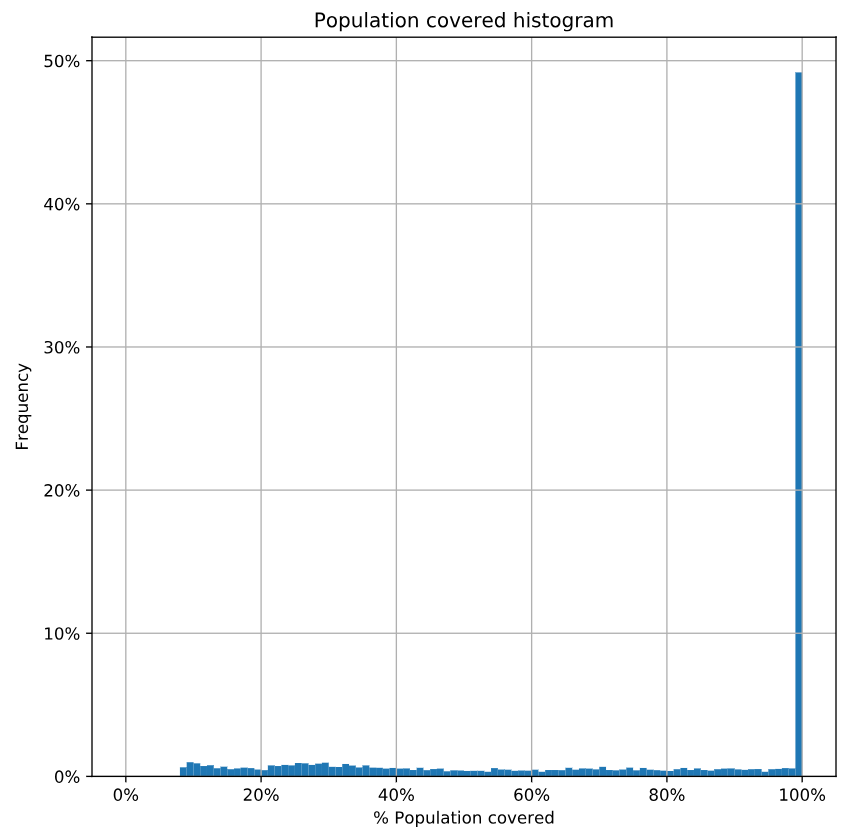
\includegraphics[width=0.80\textwidth]{./media/image45.png}
		\caption{700 MHz densification. Histogram: Population covered. Source: Author}
	\end{Center}
\end{figure}


%%%%%%%%%%%%%%%%%%%% Figure/Image No: 6 Ends here %%%%%%%%%%%%%%%%%%%%

This test uses the baseline population growth scenario, the baseline user-speed growth scenario, and the \textit{�More profitable first�} coverage obligation option with a speed of 2 Mbps. As it can be seen in the histogram, almost half of the PCDs fulfil their coverage obligations completely, but the other half cannot.\par

Combining the results of the histogram with the investment per year graph, it can be inferred that the telecom operator has enough budget to continue with the investments, but it cannot due to technical limitations. In this case, the telecom operator can only use the 700 MHz band and its capacity is limited. Half of the PCDs demand less than the maximum capacity of the band and the rest have only a portion of the coverage obligation fulfilled.\par

\subsection*{Technology upgrades}
%\addcontentsline{toc}{subsection}{Technology upgrades}
The code also allows one to see the technology upgrades of every region of the country. The following chart represents the technology upgrades made using the 700 MHz intervention. It uses the baseline population growth scenario, the baseline user-speed growth scenario, and the \textit{�More profitable first�} coverage obligation with a speed of 2 Mbps. As can be seen, the distribution of the deployment of base stations is not homogeneous since the London region is much more populated than areas from Wales or Scotland.\par



%%%%%%%%%%%%%%%%%%%% Figure/Image No: 7 starts here %%%%%%%%%%%%%%%%%%%%

\begin{figure}[H]
	\begin{Center}
		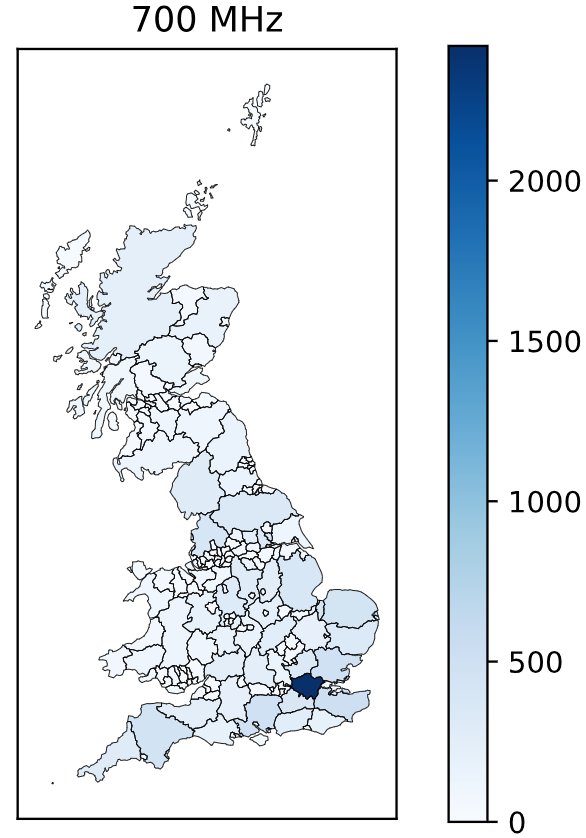
\includegraphics[width=0.50\textwidth]{./media/image46.png}
		\caption{700 MHz densification. Map: Technology upgrades. Source: Author}
	\end{Center}
\end{figure}


%%%%%%%%%%%%%%%%%%%% Figure/Image No: 7 Ends here %%%%%%%%%%%%%%%%%%%%

\subsection*{Capacity margin}
%\addcontentsline{toc}{subsection}{Capacity margin}
The section �Population Covered� discussed the\ relation between the capacity installed and the coverage obligation. Now, we study the capacity and demand parameters and its relation, the capacity margin.  The following coloured map represents the evolution of the capacity along the years.\par



%%%%%%%%%%%%%%%%%%%% Figure/Image No: 8 starts here %%%%%%%%%%%%%%%%%%%%

\begin{figure}[H]
	\begin{Center}
		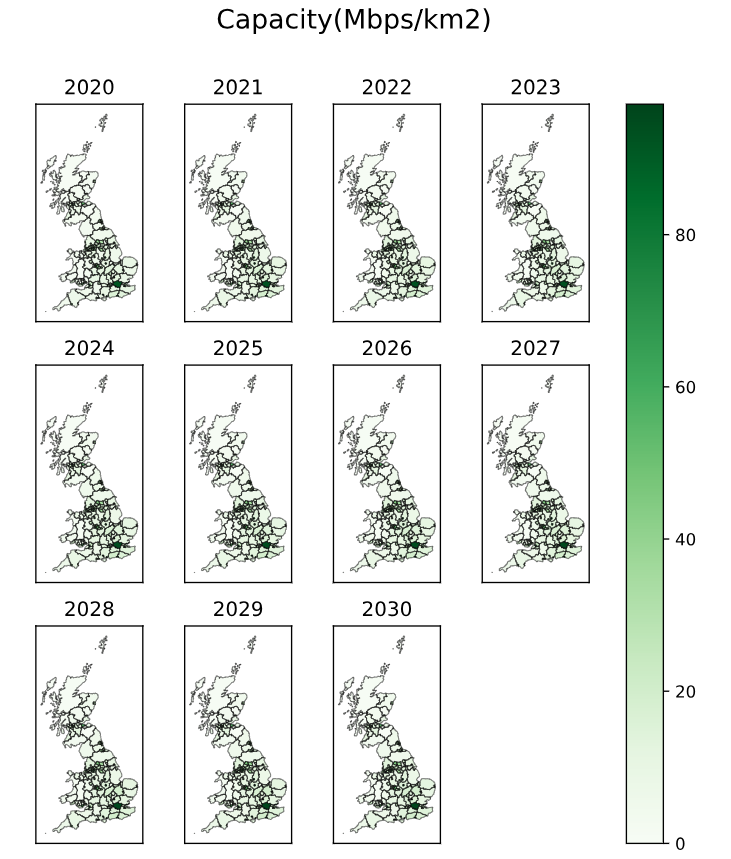
\includegraphics[width=0.9\textwidth]{./media/image47.png}
		\caption{700 MHz densification. Map: Capacity evolution. Source: Author}
	\end{Center}
\end{figure}


%%%%%%%%%%%%%%%%%%%% Figure/Image No: 8 Ends here %%%%%%%%%%%%%%%%%%%%

This map is calculated using the baseline population growth scenario, the baseline user-speed growth scenario, and the \textit{�More profitable first�} coverage obligation with a speed of 2 Mbps. It represents the capacity in Mbps per km\textsuperscript{2} installed at the end of each year and allows to see the evolution of the investment but also to see how much capacity was installed in each region at the beginning of the simulation. Note that if the reader wants to back-calculate the maximum population that could be satisfied using a capacity of 50 Mbps per km\textsuperscript{2} the conversion is not direct since they should consider the overbooking factor, the market share of the operator, etc. The following map represents the evolution of the demand over the years using the same simulation:\par



%%%%%%%%%%%%%%%%%%%% Figure/Image No: 9 starts here %%%%%%%%%%%%%%%%%%%%

\begin{figure}[H]
	\begin{Center}
		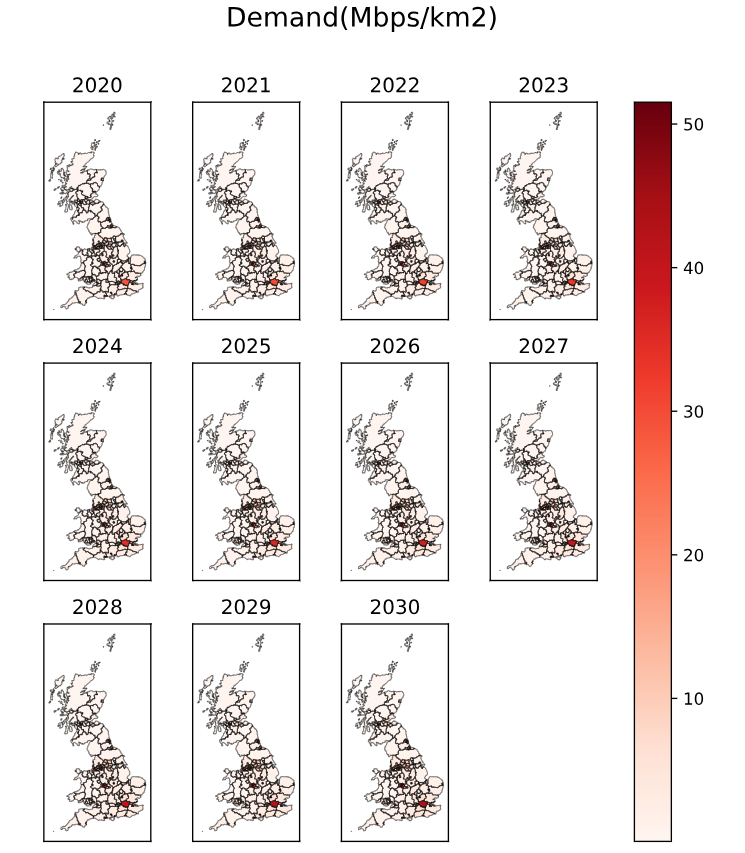
\includegraphics[width=0.90\textwidth]{./media/image48.png}
		\caption{700 MHz densification. Map: Demand evolution. Source: Author}
	\end{Center}
\end{figure}


%%%%%%%%%%%%%%%%%%%% Figure/Image No: 9 Ends here %%%%%%%%%%%%%%%%%%%%

Finally, the following coloured map calculates the subtraction of the demand from the capacity values and represents the amount of capacity in Mbps per km\textsuperscript{2} that each region lacks or has extra. This is the value that, without coverage obligations, the telecom operators normally use to check which are the highest priority areas to invest.\par


%%%%%%%%%%%%%%%%%%%% Figure/Image No: 10 starts here %%%%%%%%%%%%%%%%%%%%

\begin{figure}[H]
	\begin{Center}
		\includegraphics[width=0.90\textwidth]{./media/image49.png}
		\caption{700 MHz densification. Map: Capacity margin evolution. Source: Author}
	\end{Center}
\end{figure}


%%%%%%%%%%%%%%%%%%%% Figure/Image No: 10 Ends here %%%%%%%%%%%%%%%%%%%%
\subsection*{Total costs}
%\addcontentsline{toc}{subsection}{Total costs}
The previous analysis was executed considering that the telecom operator has a limited amount of money available to invest every year. As we want to be sure if the operator is limited by investment force or technical requirements, I have run a new execution of the code without limits in the annual budget and the results are the same. The problem of using only the 700 MHz band is that telecom operators cannot satisfy the demand.\par

\section{Capacity expansion strategies comparison}
%\subsection*{Capacity expansion strategies comparison}
%\addcontentsline{toc}{section}{Capacity expansion strategies comparison}
The previous section was related to the analysis of just the capacity expansion strategy created in this work. Now I am going to compare it to the rest of them and to test the impact that different capacity expansion strategies have on the development of the telecommunication infrastructure. The capacity expansion strategies are: �\textit{Minimum intervention�, �Spectrum integration�, �700 MHz spectrum integration�, �Small cells strategy�, �Hybrid strategy� }and\textit{ �700 MHz densification�}. These tests will use the baseline population growth scenario, the baseline user-speed growth scenario, and the \textit{�More profitable first�} coverage obligation with a speed of 2 Mbps.\par

\subsection*{Population covered}
%\addcontentsline{toc}{subsection}{Population covered}
The population covered is the first output that we analyse. The following graph represents the evolution of the percentage covered per year and gives us an idea of the maximum percentage that the capacity expansion strategy is capable of providing in the given scenario. \par

%%%%%%%%%%%%%%%%%%%% Figure/Image No: 11 starts here %%%%%%%%%%%%%%%%%%%%

\begin{figure}[H]
	\begin{Center}
		\includegraphics[width=0.95\textwidth]{./media/image50.png}
		\caption{Capacity strategies comparison. Graph: Population covered. Source: Author}
	\end{Center}
\end{figure}


%%%%%%%%%%%%%%%%%%%% Figure/Image No: 11 Ends here %%%%%%%%%%%%%%%%%%%%

This graph represents the population covered after the interventions of any one year. This way, the starting percentage is 32$\%$  and is the same for all the interventions. As can be seen in the plot, not all the lines reach 100$\%$  of the population covered by 2030. Apart from �\textit{Minimum intervention�}, that cannot build new assets and, therefore, does not increase the population covered, there are two main groups of strategies: those that can build new assets (\textit{�700 MHz densification�}, \textit{�Small cells strategy� }and \textit{�Hybrid strategy�}) and those that cannot (\textit{�Spectrum integration� }and \textit{�700 MHz spectrum integration �}).\par

In the graph, only \textit{�Small cells strategy� }and \textit{�Hybrid strategy�} could potentially reach the 100$\%$  population covered while the rest only raise the percentage from 32$\%$  to 70-90$\%$ . This is because, while the small cells related strategies increase the percentage of population covered during the whole simulation, the rest stop growing around 2023-24. This is because of two factors: (I) the extremely good capacity of the small cells in the model and (II) that MINERVA allows densification strategies, which means creating more sites for small cells until all the demand is satisfied. If these strategies really achieve the 100$\%$  population covered will be studied later.\par

\textit{�700 MHz densification�} is also allowed to create new sites, but the 700 MHz band has less bandwidth than 3.7 GHz and, therefore, using only this band is not enough to meet the demand in some regions. Finally, the rest of the strategies are not allowed to create new sites, just to upgrade those sites that already have legacy technologies (Such as 2G and 3G). These strategies cannot satisfy the demand either but due to two different factors:\par

\begin{itemize}
	\item Checking the list of assets provided in the original model, there is a part of the PCDs that have no assets at the beginning of the execution in the whole PCD. This is not an issue of the behaviour of the code, but of the database from which this information was obtained for the NISMOD project. Half of the interventions (Except \textit{�Small cells strategy�, �Hybrid strategy� and �700 MHz densification�}) cannot build new assets, and, therefore, strategies that only use this type of interventions are affected by this limitation.\par

	\item The other factor is that there is a limit to the capacity that one band can provide. Strategies that only use one or two bands, such as \textit{�700 MHz spectrum integration �} and \textit{�700 MHz densification�} are mainly affected by this limitation in the most densely populated regions.
\end{itemize}\par

\textit{�Spectrum integration�} strategy grows with the similar rate than the other macrocell related strategies, but when they stop growing, the \textit{�Spectrum integration� }strategy continues the rise a little bit more and manages to reach around the 90$\%$  of the population. This is because it is the only strategy allowed to build assets with the 3,500 MHz band which has the bigger bandwidth and hence provides more capacity.\par

\subsection*{Investment}
%\addcontentsline{toc}{subsection}{Investment}
The second output that we will review is the comparison of costs. The following graph compares the investment effort that the telecom operator would make depending on the capacity expansion strategy. This graph also uses the baseline population growth scenario, the baseline user-speed growth scenario, and the \textit{�More profitable first�} coverage obligation option with a speed of 2 Mbps.\par


%%%%%%%%%%%%%%%%%%%% Figure/Image No: 12 starts here %%%%%%%%%%%%%%%%%%%%

\begin{figure}[H]
	\begin{Center}
		\includegraphics[width=0.95\textwidth]{./media/image51.png}
		\caption{Capacity strategies comparison. Graph: Total cost. Source: Author}
	\end{Center}
\end{figure}


%%%%%%%%%%%%%%%%%%%% Figure/Image No: 12 Ends here %%%%%%%%%%%%%%%%%%%%

The given graph represents the cost that takes to reach a specific population covered percentage for each capacity strategy. As can be seen in the plot, none of the lines reaches 100$\%$  since they cannot cover the whole population by 2030.\par

From the beginning to 75$\%$  covered, which are the urban and suburban areas, the marginal cost to increase by 1$\%$  is similar for most of the strategies. The $``$Small cells$"$  strategy is a little bit more expensive since it starts building small cells directly, while the rest of strategies use LTE or 700 MHz bands before. After 75$\%$  of the population, the cost of both small cells strategies grows drastically and makes it not affordable.\par

The graph also reflects the differences between all the strategies that only use macrocell bands (700, 800, 2,600, 3,500 MHz). \textit{�Spectrum integration�} is the best strategy since can use all the bands and the only one that can use the 3,500 MHz band. Hence, the gap from 85$\%$  of the population covered to 95$\%$  is just thanks to adding this band, which helps in those regions where the rest of the bands combined were not enough. \textit{�700 MHz spectrum integration� }has LTE and 700 MHz, while \textit{�700 MHz densification�} only uses the 700 MHz. For this reason, despite \textit{�700 MHz densification�} can create new sites and can provide connectivity in places where it is not possible with the other strategies, \textit{�700 MHz spectrum integration� }is capable of covering much more population at the end of the execution. It is important to remember that these strategies are not limited by the budget of the operator, but by the technical issues explained above.\par


\subsection*{Capacity margin}
%\addcontentsline{toc}{subsubsection}{Capacity margin}
The capacity margin is the third and last output that we are going to evaluate, and it is related to the difference between the absolute value of the capacity of the network and the absolute value of the demand of the network in Mbps/km\textsuperscript{2}. This is not related to the coverage obligations, but to the estimated demand of the population. The following graph uses the baseline population growth scenario, the baseline user-speed growth scenario, and the \textit{�More profitable first�} coverage obligation option with a speed of 2 Mbps.\par



%%%%%%%%%%%%%%%%%%%% Figure/Image No: 13 starts here %%%%%%%%%%%%%%%%%%%%

\begin{figure}[H]
	\begin{Center}
		\includegraphics[width=0.95\textwidth]{./media/image52.png}
		\caption{Capacity strategies comparison. Graph: Capacity margin. Source: Author}
	\end{Center}
\end{figure}


%%%%%%%%%%%%%%%%%%%% Figure/Image No: 13 Ends here %%%%%%%%%%%%%%%%%%%%

The most interesting strategy for a telecom operator is to have high population covered, with the minimum cost possible and with a positive capacity margin but as small as possible. Otherwise, it would mean that the operator made a big investment that is not been harnessed. \par

This graph shows the same differences that we could see before. There is a strong difference between strategies that use the small cells intervention and those that do not. Small cells are good but expensive and using just small cells comprise a huge waste of budget in the less populated areas.\par

\subsection*{Total costs }
%\addcontentsline{toc}{subsection}{Total costs }
The model calculates that a telecom operator with a market share of 30$\%$  of the population that use mobile broadband services have approximately �600,000,000 per year to invest in new assets and operate them. The purpose of this section is to verify which of the limitations that we found in the previous charts are due to technical or monetary restrictions. In the case of the limitations that were because of the budget, this model also shows the total amount of money that would be needed.\par

The following chart represents the same information as the cost section, which is the cost that takes to achieve certain population covered, but removing the budget limitations:\par



%%%%%%%%%%%%%%%%%%%% Figure/Image No: 14 starts here %%%%%%%%%%%%%%%%%%%%

\begin{figure}[H]
	\begin{Center}
		\includegraphics[width=0.95\textwidth]{./media/image53.png}
		\caption{Capacity strategies comparison. Graph: Total cost without budget limitation. Source: Author}
	\end{Center}
\end{figure}


%%%%%%%%%%%%%%%%%%%% Figure/Image No: 14 Ends here %%%%%%%%%%%%%%%%%%%%

As can be seen, the graph is similar to the previous one, but now the \textit{�Small cells strategy�} and the \textit{�Hybrid strategy�} strategies reach the 100$\%$  population covered, which confirms the previous analysis. \par

The maximum budget that the operator can spend in 11 years (From 2020 to 2030) is �6,600,000,000 which was the maximum value of the Y-axis in the budget limited cost chart. Now, the total cost is �20,600,000,000 which is three times the budget that the operator has. In fact, it is also important to remark that rising the population covered from 90$\%$  to 100$\%$  implies spending more than two times of what it took to rise from the original coverage to 90$\%$ .\par

The rest of strategies are not modified since they were not limited by budget but by technical constraints.\par

The capacity margin is also affected in this case and the results are not good for the small cells since the final capacity margin is too big. The following graph represents the capacity margin per year. As the budget is not limited, the operator builds all the assets in 2020, but it shows the differences between strategies clearly. \par



%%%%%%%%%%%%%%%%%%%% Figure/Image No: 15 starts here %%%%%%%%%%%%%%%%%%%%

\begin{figure}[H]
	\begin{Center}
		\includegraphics[width=0.95\textwidth]{./media/image54.png}
		\caption{Capacity strategies comparison. Graph: Capacity margin without budget limitation. Source: Author}
	\end{Center}
\end{figure}


%%%%%%%%%%%%%%%%%%%% Figure/Image No: 15 Ends here %%%%%%%%%%%%%%%%%%%%

The important point of this graph is that it allows us to see which is the maximum capacity margin for each capacity expansion strategy. In the previous capacity margin graph, the small cells related strategies did not stop growing their margin. In this graph, we can see the real final value of the strategies. However, the rest of the strategies do not increase their margin in spite of having an unlimited budget. This is mainly because these strategies have a technical limitation, not a budget limitation. \par


\section{Coverage obligation sets}
%\subsection*{Coverage obligation options}
%\addcontentsline{toc}{section}{Coverage obligation sets}
In this section, a detailed study of the coverage obligation sets will be provided. The aim is to be able to understand the implications that each of them has in the development of the new mobile broadband assets deployment in the country. In the previous chapter, we analysed the �\textit{More profitable first�} option, which is the original version. Now, four new sets are analysed: �\textit{Priority areas first�, �Less profitable areas first�, �Only rural areas� and �Nation-balanced�.} Finally, we will compare them using two types of capacity expansion strategies to assess the advantages and disadvantages of each of them.\par

\subsection{Priority areas first}
This is the first of the coverage obligation sets and divides all the PCDs into two sections: First, it invests in the 18$\%$  less densely populated PCDs, starting in the most densely populated of those and later it invests in the rest of them, starting in the most densely populated of this subgroup. It is explained in higher detail in the previous chapter. We are going to analyse how it behaves using two different capacity expansion strategies: (I) \textit{�Hybrid strategy�}, which makes use of all the possible interventions, and (II) \textit{�700 MHz densification�}, which is the strategy that I have designed in this thesis.\par

\subsubsection*{�Hybrid strategy�}
%\addcontentsline{toc}{subsubsection}{�Hybrid strategy�}
The first graph that we are going to analyse is the cost that takes to increment the population covered. As \textit{�Priority areas first�} starts in with the 18$\%$  less densely populated and, therefore, less profitable, the graph has a different shape than the one that had with \textit{�Most profitable first�:}\par



%%%%%%%%%%%%%%%%%%%% Figure/Image No: 1 starts here %%%%%%%%%%%%%%%%%%%%

\begin{figure}[H]
	\begin{Center}
		\includegraphics[width=1\textwidth]{./media/image55.png}
		\caption{Priority areas first - Hybrid strategy. Graph: Cost. Source: Author}
	\end{Center}
\end{figure}


%%%%%%%%%%%%%%%%%%%% Figure/Image No: 1 Ends here %%%%%%%%%%%%%%%%%%%%

First, we have to cover the most rural areas and, therefore, the curve is so steep. After the 18$\%$  population is covered, the slope of the curve gets reduced immediately, because we start to cover the most densely populated. When it reaches the 90$\%$  of the population, the marginal cost escalates because we change to the rural geotype again, which have worse propagation properties.\par

This combination of coverage obligation set and capacity strategy has two main disadvantages: (i) it forces the operator to invest in all of the PCDs, but starting in the less-profitable 18$\%$  and (ii) the only option for those PCDs that have no assets deployed at the beginning is to create a full small cells network, which has an exorbitant cost. The result is that the percentage of population covered raises just a little, despite the operator invests all it can for eleven years:\par



%%%%%%%%%%%%%%%%%%%% Figure/Image No: 2 starts here %%%%%%%%%%%%%%%%%%%%

\begin{figure}[H]
	\begin{Center}
		\includegraphics[width=0.95\textwidth]{./media/image56.png}
		\caption{Priority areas first - Hybrid strategy. Graph: Population covered (left) and investment (right). Source: Author}
	\end{Center}
\end{figure}


%%%%%%%%%%%%%%%%%%%% Figure/Image No: 2 Ends here %%%%%%%%%%%%%%%%%%%%

The evolution of the capacity margin over the years is also an important output when it is combined with the investment effort. If the investment effort is huge, as it is here, the capacity margin should raise, reflecting it. In this case, it does not happen since the effort is done in the least profitable areas. The following chart represents how little this output grows nationwide:\par



%%%%%%%%%%%%%%%%%%%% Figure/Image No: 3 starts here %%%%%%%%%%%%%%%%%%%%

\begin{figure}[H]
	\begin{Center}
		\includegraphics[width=0.70\textwidth]{./media/image57.png}
		\caption{Priority areas first - Hybrid strategy. Graph: Capacity margin. Source: Author}
	\end{Center}
\end{figure}


%%%%%%%%%%%%%%%%%%%% Figure/Image No: 3 Ends here %%%%%%%%%%%%%%%%%%%%


The problem of the previous graph is that it aggregates the capacity margin of all the areas and it does not help us to see the differences between areas. The following two histograms represent the probability of a specific capacity margin and its cumulative distribution function, which represent the probability of having at least a specific margin in each PCD: \par



%%%%%%%%%%%%%%%%%%%% Figure/Image No: 4 starts here %%%%%%%%%%%%%%%%%%%%

\begin{figure}[H]
	\begin{Center}
		\includegraphics[width=0.95\textwidth]{./media/image58.png}
		\caption{Priority areas first - Hybrid strategy. Histogram: Capacity margin (left) and CDF (right). Source: Author}
	\end{Center}
\end{figure}


%%%%%%%%%%%%%%%%%%%% Figure/Image No: 4 Ends here %%%%%%%%%%%%%%%%%%%%

As it can be seen in the graph, the distribution function of the capacity margin has two main parts: (I) A Gaussian with the mean in 0 and low variance and (II) a group of PCDs whose capacity margin is around 600 Mbps/km2. This is a clear indicator of the low suitability of this combination since, instead of gradually giving more capacity to all the PCDs, it gives a huge capacity to only some of them, creating two distinct groups.\par

The distribution of the percentage of population covered along the PCDs is another value that we are going to consider, and we will see that its distribution is quite similar to the capacity margin one. \par



%%%%%%%%%%%%%%%%%%%% Figure/Image No: 5 starts here %%%%%%%%%%%%%%%%%%%%

\begin{figure}[H]
	\begin{Center}
		\includegraphics[width=0.95\textwidth]{./media/image59.png}
		\caption{Priority areas first - Hybrid strategy. Histogram: Population covered (left) and CDF (right). Source: Author}
	\end{Center}
\end{figure}


%%%%%%%%%%%%%%%%%%%% Figure/Image No: 5 Ends here %%%%%%%%%%%%%%%%%%%%

The problem with the population covered is that, as we spend a lot of resources in the priority areas, there is no more budget for the more profitable ones. Fifty per cent of the PCDs has 0$\%$  population covered since no money is invested there. Almost 30$\%$  of the areas have more than the capacity needed and are covered at 100$\%$  and the rest have an intermediate capacity thanks to the assets that they had already built before the execution of the simulation.\par

Now, we are going to evaluate these parameters using some coloured maps, so we can see exactly the differences between regions in the UK map. First, we are going to see the investment per year and LAD. It is important to notice that the most densely populated regions never receive investments, while the money is spent only in some regions.\par



%%%%%%%%%%%%%%%%%%%% Figure/Image No: 6 starts here %%%%%%%%%%%%%%%%%%%%

\begin{figure}[H]
	\begin{Center}
		\includegraphics[width=0.85\textwidth]{./media/image60.png}
		\caption{Priority areas first - Hybrid strategy. Map: Cost. Source: Author}
	\end{Center}
\end{figure}


%%%%%%%%%%%%%%%%%%%% Figure/Image No: 6 Ends here %%%%%%%%%%%%%%%%%%%%


This distribution of the investment has an impact on two metrics: the population covered and the capacity margin. These maps represent the evolution of those over the years. As it can be seen in the capacity margin maps, it gets too high in some regions (200Mbps/km\textsuperscript{2} in some cases), while it remains as it was at the beginning in the ones that have more population.\par



%%%%%%%%%%%%%%%%%%%% Figure/Image No: 7 starts here %%%%%%%%%%%%%%%%%%%%

\begin{figure}[H]
	\begin{Center}
		\includegraphics[width=0.95\textwidth]{./media/image61.png}
		\caption{Priority areas first - Hybrid strategy. Map: Capacity margin. Source: Author}
	\end{Center}
\end{figure}


%%%%%%%%%%%%%%%%%%%% Figure/Image No: 7 Ends here %%%%%%%%%%%%%%%%%%%%

The following map represents the evolution of the population covered parameter. As it can be seen, this output improves over the course of time, but not with the same growth rate that other capacity expansion strategies have.\par


%%%%%%%%%%%%%%%%%%%% Figure/Image No: 8 starts here %%%%%%%%%%%%%%%%%%%%

\begin{figure}[H]
	\begin{Center}
		\includegraphics[width=1\textwidth]{./media/image62.png}
		\caption{Priority areas first - Hybrid strategy. Map: Population covered. Source: Author}
	\end{Center}
\end{figure}


%%%%%%%%%%%%%%%%%%%% Figure/Image No: 8 Ends here %%%%%%%%%%%%%%%%%%%%


\paragraph*{No budget limitation}
%\addcontentsline{toc}{paragraph}{No budget limitation}
Using the same strategy than above, but removing the budget limitation allows us to see how much it would really cost to cover all the population with the obligation and to satisfy the end-user speed demand. The following graph represents the marginal cost that increasing the percentage of population covered implies:\par



%%%%%%%%%%%%%%%%%%%% Figure/Image No: 9 starts here %%%%%%%%%%%%%%%%%%%%

\begin{figure}[H]
	\begin{Center}
		\includegraphics[width=0.7\textwidth]{./media/image63.png}
		\caption{Priority areas first - Hybrid strategy. Graph: Cost without budget limitation. Source: Author}
	\end{Center}
\end{figure}


%%%%%%%%%%%%%%%%%%%% Figure/Image No: 9 Ends here %%%%%%%%%%%%%%%%%%%%


This graph shows that reaching the 100$\%$  is possible using this combination, but the problem is that at the beginning it makes a strong effort in developing regions that are not so profitable. The total costs are around 3 times more than the budget of the telecom operator and, with the real budget, it would only reach the 42$\%$ .\par

\subsubsection*{�700 MHz densification� }
%\addcontentsline{toc}{subsubsection}{�700 MHz densification� }
Now, we are going to test how good the \textit{�700 MHz densification�} strategy works in conjunction with the �\textit{Priority areas first�} coverage obligation set. The major advantage of this strategy is that it can only create assets in the 700 MHz and that the maximum site density of this band is considerably lower than in the case of the small cells. As it can be seen in the following chart, in this case, the investment is not equally during the whole period. \par



%%%%%%%%%%%%%%%%%%%% Figure/Image No: 10 starts here %%%%%%%%%%%%%%%%%%%%

\begin{figure}[H]
	\begin{Center}
		\includegraphics[width=0.55\textwidth]{./media/image64.png}
		\caption{Priority areas first - 700 MHz densification. Graph: Investment. Source: Author}
	\end{Center}
\end{figure}


%%%%%%%%%%%%%%%%%%%% Figure/Image No: 10 Ends here %%%%%%%%%%%%%%%%%%%%


This strategy meets the coverage obligations� investment in the fourth year and after that, it only needs to invest to satisfy the end-user speed demand. However, this graph cannot be understood without analysing the evolution of the capacity margin and population covered. The following graphs represent these values aggregated by year:\par



%%%%%%%%%%%%%%%%%%%% Figure/Image No: 11 starts here %%%%%%%%%%%%%%%%%%%%

\begin{figure}[H]
	\begin{Center}
		\includegraphics[width=0.9\textwidth]{./media/image65.png}
		\caption{Priority areas first - 700 MHz densification. Graph: Capacity margin (left) and population covered (right). Source: Author}
	\end{Center}
\end{figure}


%%%%%%%%%%%%%%%%%%%% Figure/Image No: 11 Ends here %%%%%%%%%%%%%%%%%%%%

Both outputs show better values than with the �\textit{Hybrid strategy�} strategy since, using less budget, the capacity margin does not growth so much. This means that all the investment effort is done in those areas that need it, but the population covered percentage grows faster and further than in the previous case. The following histograms also show the distribution of the capacity and the percentage of the population covered across the country. The graph on the left shows the CDF of the capacity margin histogram and the one on the right is the histogram of the population covered.\par



%%%%%%%%%%%%%%%%%%%% Figure/Image No: 12 starts here %%%%%%%%%%%%%%%%%%%%

\begin{figure}[H]
	\begin{Center}
		\includegraphics[width=0.9\textwidth]{./media/image66.png}
		\caption{Priority areas first - 700 MHz densification. Graph: Capacity margin CDF (left) and population covered histogram (right). Source: Author}
	\end{Center}
\end{figure}


%%%%%%%%%%%%%%%%%%%% Figure/Image No: 12 Ends here %%%%%%%%%%%%%%%%%%%%


The result is that the capacity margin is mainly around the 0 Mbps/km\textsuperscript{2} which is not a bad result since only 30$\%$  of the PCDs have less margin than 0 Mbps/km\textsuperscript{2} and only 8$\%$  are over it. The population covered histogram represents that all the PCDs received some investment. For half of them, the capacity installed was not enough and require more frequency bands in order to have enough capacity to satisfy the coverage obligation requirements. Despite this, the overall population coverage percentage is really good and most of the PCDs have 100$\%$  or values near to this:\par



%%%%%%%%%%%%%%%%%%%% Figure/Image No: 13 starts here %%%%%%%%%%%%%%%%%%%%

\begin{figure}[H]
	\begin{Center}
		\includegraphics[width=0.95\textwidth]{./media/image67.png}
		\caption{Priority areas first - 700 MHz densification. Map: Population covered. Source: Author}
	\end{Center}
\end{figure}


%%%%%%%%%%%%%%%%%%%% Figure/Image No: 13 Ends here %%%%%%%%%%%%%%%%%%%%


This coloured map is significantly better in terms of coverage than the results of the \textit{�Hybrid strategy�}.\par

Finally, the following graph shows the cost of incrementing the percentage of population covered. It is important to stress that the differences in the results between this graph and the one in section 4.1 are only because of the selected coverage obligation set. In this case, investment starts in some of the less-profitable PCDs and, therefore, the graph starts with a higher slope. Then, after the 18$\%$ , the slope is reduced.\par


%%%%%%%%%%%%%%%%%%%% Figure/Image No: 14 starts here %%%%%%%%%%%%%%%%%%%%

\begin{figure}[H]
	\begin{Center}
		\includegraphics[width=0.75\textwidth]{./media/image68.png}
		\caption{Priority areas first - 700 MHz densification. Graph: Population covered vs. cost. Source: Author}
	\end{Center}
\end{figure}


%%%%%%%%%%%%%%%%%%%% Figure/Image No: 14 Ends here %%%%%%%%%%%%%%%%%%%%


The 700 MHz band is aimed at covering large portions of fields with lower costs and not at providing huge end-user speeds. Hence, this capacity expansion strategy has better results in this situation, where the coverage obligation set starts investing in the less populated areas.\par

\paragraph*{No budget limitation}
\addcontentsline{toc}{paragraph}{No budget limitation}
In this case, there is no difference between having a budget limitation or not since not all the budget is spent even when there is a budget limit. Therefore, almost all the graphs in the previous section also apply to this situation. Obviously, the only graphs that do not match are those that are related to the evolution over the years since, in this case, all the investment is done the first year.\par





















\subsection{Less profitable areas first}
Now, we are going to analyse the second coverage obligation set developed in this study. This strategy allows the telecom operator to build new assets in a PCD only if it has already invested in all of the PCDs with less population density. We are going to test how it behaves for two different capacity expansion strategies: \textit{�Hybrid strategy�} and \textit{�700 MHz densification�.}\par

\subsubsection*{�Hybrid strategy�}
%\addcontentsline{toc}{subsubsection}{�Hybrid strategy�}
Although I am not showing the investment evolution again, the situation is similar as in \textit{�Priority areas first�. }Using the �\textit{Hybrid strategy}� the telecom operator invests to the fullest capacity for all the years and even then, the results are not what was expected. The following graphs represent the evolution of the capacity margin, on the left, and the population covered over the years, on the right:\par



%%%%%%%%%%%%%%%%%%%% Figure/Image No: 15 starts here %%%%%%%%%%%%%%%%%%%%

\begin{figure}[H]
	\begin{Center}
		\includegraphics[width=0.90\textwidth]{./media/image69.png}
		\caption{Less profitable areas first - Hybrid strategy. Graph: Capacity margin (left) and population covered (right). Source: Author}
	\end{Center}
\end{figure}


%%%%%%%%%%%%%%%%%%%% Figure/Image No: 15 Ends here %%%%%%%%%%%%%%%%%%%%

Capacity margin grows less than in the previous coverage obligation set. This could be because the telecom operator is investing in the most interesting places, but the reason is that resources are so wasted that capacity margin does not grow either. Population covered has similar values as in the previous obligation. \par



%%%%%%%%%%%%%%%%%%%% Figure/Image No: 16 starts here %%%%%%%%%%%%%%%%%%%%

\begin{figure}[H]
	\begin{Center}
		\includegraphics[width=0.90\textwidth]{./media/image70.png}
		\caption{Less profitable areas first - Hybrid strategy. Graph: Capacity margin CDF (left) and population covered histogram (right). Source: Author}
	\end{Center}
\end{figure}


%%%%%%%%%%%%%%%%%%%% Figure/Image No: 16 Ends here %%%%%%%%%%%%%%%%%%%%


As it can be seen, the situation is very similar to the previous coverage obligation set. Capacity margin per PCD is mainly about the 0Mbps/km\textsuperscript{2}, although there is a group of 10$\%$  of the PCDs that have too high capacity margin, about 600Mbps/km\textsuperscript{2} and this waste of resources is what penalizes this strategy. Moreover, we can see in the graph on the right that more than 40$\%$  of the PCDs received no investment and that only 35$\%$  of the PCDs have all of its population with the 2Mbps that the coverage obligation demands.\par

The following coloured map shows the money that has been spent in each LAD during all the execution time. It represents the problem of the unbalanced investment clearly: Most of the investment effort was made in PCDs that are not the most important nor the most densely populated.\par


%%%%%%%%%%%%%%%%%%%% Figure/Image No: 17 starts here %%%%%%%%%%%%%%%%%%%%

\begin{figure}[H]
	\begin{Center}
		\includegraphics[width=0.55\textwidth]{./media/image71.png}
		\caption{Less profitable areas first - Hybrid strategy. Map: Total cost. Source: Author}
	\end{Center}
\end{figure}


%%%%%%%%%%%%%%%%%%%% Figure/Image No: 17 Ends here %%%%%%%%%%%%%%%%%%%%


This leads us to the graph that compares the population covered by the cost that takes to reach this specific percentage of population covered. As it can be seen, starting with 35$\%$  of the population already fulfilling the coverage obligations, this strategy just increments the coverage by 10$\%$  while it is investing all the resources available.\par



%%%%%%%%%%%%%%%%%%%% Figure/Image No: 18 starts here %%%%%%%%%%%%%%%%%%%%

\begin{figure}[H]
	\begin{Center}
		\includegraphics[width=0.73\textwidth]{./media/image72.png}
		\caption{Less profitable areas first - Hybrid strategy. Graph: Population covered vs. cost. Source: Author}
	\end{Center}
\end{figure}


%%%%%%%%%%%%%%%%%%%% Figure/Image No: 18 Ends here %%%%%%%%%%%%%%%%%%%%


In order to have a full picture of this case, the following coloured maps represent the evolution of the coverage obligations over the years and how the investment effort was focused on the bigger LADs, which have normally less population density.\par



%%%%%%%%%%%%%%%%%%%% Figure/Image No: 19 starts here %%%%%%%%%%%%%%%%%%%%

\begin{figure}[H]
	\begin{Center}
		\includegraphics[width=0.75\textwidth]{./media/image73.png}
		\caption{Less profitable areas first - Hybrid strategy. Map: Population covered. Source: Author}
	\end{Center}
\end{figure}


%%%%%%%%%%%%%%%%%%%% Figure/Image No: 19 Ends here %%%%%%%%%%%%%%%%%%%%


As a summary, this coverage obligation set has the same investment effort than �\textit{Priority areas first�} and the increment of the percentage of population covered is similar, but the capacity margin does not increase as much as it does in the other set. Hence, this combination is even less interesting for the telecom operator and the policymakers than the previous one.\par

\paragraph*{No budget limitation}
%\addcontentsline{toc}{paragraph}{No budget limitation}
As it happens with the previous coverage obligation set, using this capacity expansion strategy and disabling the budget limit would allow the telecom operator to invest until it reaches the 100$\%$  of the population covered. The reason why this strategy does not reach the 100$\%$  with the budget limit is that its investments are not efficient and, therefore, the normal budget is not enough. The following graph represents the total investment needed to reach the 100$\%$  of the population covered:\par



%%%%%%%%%%%%%%%%%%%% Figure/Image No: 20 starts here %%%%%%%%%%%%%%%%%%%%

\begin{figure}[H]
	\begin{Center}
		\includegraphics[width=0.75\textwidth]{./media/image74.png}
		\caption{Less profitable areas first - Hybrid strategy. Graph: Population covered vs. cost with budget limit. Source: Author}
	\end{Center}
\end{figure}


%%%%%%%%%%%%%%%%%%%% Figure/Image No: 20 Ends here %%%%%%%%%%%%%%%%%%%%


As it can be seen, the operator would need approximately 3 times the budget estimated for the period. It is also interesting to point out that the curve is smooth, without drastic changes in the direction of the curve, since all the PCDs are ordered according to the population density.\par

\subsubsection*{�700 MHz densification�}
%\addcontentsline{toc}{subsubsection}{�700 MHz densification�}
In this section, we are going to evaluate the most interesting outputs of the \textit{�700 MHz densification� }strategy combined with the\textit{ �Less profitable first� }coverage obligation set. The main outputs are similar to the ones that we had when we combined this strategy with the �\textit{Priority areas first�} obligation since they order PCDs in the same way. For example, aggregation of the capacity margin, the investment and the population covered are similar:\par



%%%%%%%%%%%%%%%%%%%% Figure/Image No: 21 starts here %%%%%%%%%%%%%%%%%%%%

\begin{figure}[H]
	\begin{Center}
		\includegraphics[width=0.95\textwidth]{./media/image75.png}
		\caption{Less profitable areas first - 700 MHz densification. Graph: Capacity margin (left) and population covered (right). Source: Author}
	\end{Center}
\end{figure}


%%%%%%%%%%%%%%%%%%%% Figure/Image No: 21 Ends here %%%%%%%%%%%%%%%%%%%%


It is important to highlight that capacity margin growths during the years that the telecom operator has to invest to meet the coverage obligation and, then, this value goes down again. It is not beneficial for the telecom operator to have a high capacity margin if only 70$\%$  of the people have enough end-user speed to fulfil the coverage obligations.\par

The rest of the graphs are similar to the ones presented in the �\textit{Priority areas first�} coverage obligation, so it makes no sense to repeat them. The following coloured maps represent the evolution of the coverage obligations over the years:\par



%%%%%%%%%%%%%%%%%%%% Figure/Image No: 22 starts here %%%%%%%%%%%%%%%%%%%%

\begin{figure}[H]
	\begin{Center}
		\includegraphics[width=0.95\textwidth]{./media/image76.png}
		\caption{Less profitable areas first - 700 MHz densification. Map: Population covered. Source: Author}
	\end{Center}
\end{figure}


%%%%%%%%%%%%%%%%%%%% Figure/Image No: 22 Ends here %%%%%%%%%%%%%%%%%%%%


Despite the population covered in 2030 is the same, the evolution and the prioritization of LADs to invest first changes between these two coverage obligation sets, since the order in which the algorithm invests is different. As this algorithm starts with the very less profitable PCD, it focuses on the LADs of Scotland and Wales, investing in most regions of England later. However, the overall result is similar.\par

The last output that we are going to analyse is the relation between a certain percentage of population covered and the cost that it takes to obtain it. The following graph represents this relation:\par



%%%%%%%%%%%%%%%%%%%% Figure/Image No: 23 starts here %%%%%%%%%%%%%%%%%%%%

\begin{figure}[H]
	\begin{Center}
		\includegraphics[width=0.75\textwidth]{./media/image77.png}
		\caption{Less profitable areas first - 700 MHz densification. Graph: Population covered vs. cost. Source: Author}
	\end{Center}
\end{figure}


%%%%%%%%%%%%%%%%%%%% Figure/Image No: 23 Ends here %%%%%%%%%%%%%%%%%%%%


The results are similar to the previous ones, the curve is smooth, and it only reaches 70$\%$  of the population.\par

\paragraph*{No budget limitation}
%\addcontentsline{toc}{paragraph}{No budget limitation}
As it happens in the previous coverage obligation, the budget is not the limitation of this coverage obligation. Therefore, despite removing the budget limitation, the results are the same and the population covered vs cost graph has the same values.\par


































\subsection{Only rural areas}
This coverage obligation set defines two groups of PCDs according to their population: (I) PCDS with less than 800 inhabitants (Rural PCDs) and (II) PCDS with more than that (Urban and suburban). Then, operators have to invest first in all the PCDS of the group I before being allowed to build new assets in the group II. As we did before, we are going to see the results of simulations of this coverage obligation set using two different capacity expansion strategies with and without a budget limitation.\par

\subsubsection*{�Hybrid strategy� }
\addcontentsline{toc}{subsubsection}{�Hybrid strategy� }
This coverage obligation set is characterized by its less stringent requirements, which gives the opportunity to the telecom operators to focus earlier in building assets to satisfy the demand instead of using most of its budget in building resources to fulfil the coverage obligations. All the graphs in this section represent a simulation in which the telecom operator creates new assets to meet end-user speed demand after building all the assets of the coverage obligation.\par

The first graphs represent the evolution of the capacity margin and population covered over the years. It is important to remember that, in this simulation, the telecom operator invests all the budget available every year.\par



%%%%%%%%%%%%%%%%%%%% Figure/Image No: 24 starts here %%%%%%%%%%%%%%%%%%%%

\begin{figure}[H]
	\begin{Center}
		\includegraphics[width=0.95\textwidth]{./media/image78.png}
		\caption{Only rural areas - Hybrid strategy. Graph: Capacity margin (left) and population covered (right). Source: Author}
	\end{Center}
\end{figure}


%%%%%%%%%%%%%%%%%%%% Figure/Image No: 24 Ends here %%%%%%%%%%%%%%%%%%%%

As it can be seen, the evolution of both parameters is much better than in previous coverage obligations. Capacity margin grows rapidly, but this is not bad since the operator invests just where it considers that their users are lack of capacity (The green line represents the change from coverage obligations to demand). The percentage of population covered grows fast, as well, which is even better than the capacity margin. Note that, in this case, as coverage obligations affect so little part of the population of the country, the values of the population covered are calculated as if obligations would affect the whole country. Moreover, the reader should notice that the slope decreases as time goes by since the operator invests first in the more profitable PCDs and then continues with the less profitable ones.\par

Now, we are going to analyse the CDF of the histogram of the capacity margin and the histogram of the population covered, to see how these values are distributed along the territory and check the inequality between territories:\par



%%%%%%%%%%%%%%%%%%%% Figure/Image No: 25 starts here %%%%%%%%%%%%%%%%%%%%

\begin{figure}[H]
	\begin{Center}
		\includegraphics[width=0.95\textwidth]{./media/image79.png}
		\caption{Only rural areas - Hybrid strategy. Graph: Capacity margin CDF (left) and population covered histogram (right). Source: Author}
	\end{Center}
\end{figure}


%%%%%%%%%%%%%%%%%%%% Figure/Image No: 25 Ends here %%%%%%%%%%%%%%%%%%%%


As can be noted from the above charts, after eleven years of investment, the capacity margin of all the regions is at 0 Mbps/km\textsuperscript{2} (50$\%$  of the PCDs) or above (50$\%$  of the PCDs). Even, some of them (25$\%$ ) have a really big capacity margin, which is around 600Mbps/km\textsuperscript{2}. The problem comes with the population covered histogram since results are different from the other executions. In this case, 20$\%$  of the PCDs have no population covered since they received no investment from the telecom operator. On the contrary, almost 80$\%$  of the PCDs have a coverage percentage of 100$\%$ .\par

Now, we are going to see the evolution of the capacity margin and the percentage of population covered. This allows seeing the distribution of these parameters along the national territory:\par



%%%%%%%%%%%%%%%%%%%% Figure/Image No: 26 starts here %%%%%%%%%%%%%%%%%%%%

\begin{figure}[H]
	\begin{Center}
		\includegraphics[width=0.95\textwidth]{./media/image80.png}
		\caption{Only rural areas - Hybrid strategy. Map: Capacity margin. Source: Author}
	\end{Center}
\end{figure}


%%%%%%%%%%%%%%%%%%%% Figure/Image No: 26 Ends here %%%%%%%%%%%%%%%%%%%%


The evolution of the capacity margin is very good. Capacity margin reaches 600Mbps/km\textsuperscript{2} in some LADs, which is a lot and no LAD has the capacity margin below 0. It is important to notice that there are more improvements in England instead of been homogeneous in all the countries. The following coloured map represents the evolution of the coverage obligation:\par



%%%%%%%%%%%%%%%%%%%% Figure/Image No: 27 starts here %%%%%%%%%%%%%%%%%%%%

\begin{figure}[H]
	\begin{Center}
		\includegraphics[width=0.95\textwidth]{./media/image81.png}
		\caption{Only rural areas - Hybrid strategy. Map: Population covered. Source: Author}
	\end{Center}
\end{figure}


%%%%%%%%%%%%%%%%%%%% Figure/Image No: 27 Ends here %%%%%%%%%%%%%%%%%%%%


This time, something similar to the capacity margin happens with the percentage of population covered in each LAD: Values are better than using other coverage obligation sets, but they are focused on England, while values in Scotland and Wales are smaller.\par

Finally, we are going to analyse the population covered vs. cost graph. As it can be seen, coverage obligations only affect a little part of the whole population of the country. After an almost-vertical slope of 1$\%$  or 2$\%$  of the population, the telecom operator has fulfilled the coverage obligations and starts investing in prioritizing the profitability.\par



%%%%%%%%%%%%%%%%%%%% Figure/Image No: 28 starts here %%%%%%%%%%%%%%%%%%%%

\begin{figure}[H]
	\begin{Center}
		\includegraphics[width=0.75\textwidth]{./media/image82.png}
		\caption{Only rural areas - Hybrid strategy. Graph: Population covered vs. cost. Source: Author}
	\end{Center}
\end{figure}


%%%%%%%%%%%%%%%%%%%% Figure/Image No: 28 Ends here %%%%%%%%%%%%%%%%%%%%


In general, results are not bad, but the reality is that they are similar to the ones obtained when there are no coverage obligation sets and the policymaker allows telecom operators to decide which are the most suitable PCDs to invest. \par

\paragraph*{No budget limitation}
%\addcontentsline{toc}{paragraph}{No budget limitation}
Now we are going to see how removing the budget limitation affects the population covered. The following graph represents the same values as above, but in a simulation where there is no budget limitation.\par



%%%%%%%%%%%%%%%%%%%% Figure/Image No: 29 starts here %%%%%%%%%%%%%%%%%%%%

\begin{figure}[H]
	\begin{Center}
		\includegraphics[width=0.75\textwidth]{./media/image83.png}
		\caption{Only rural areas - Hybrid strategy. Graph: Population covered vs. cost without budget limitation. Source: Author}
	\end{Center}
\end{figure}


%%%%%%%%%%%%%%%%%%%% Figure/Image No: 29 Ends here %%%%%%%%%%%%%%%%%%%%


As it can be seen, the limitations where only due to the budget and removing this limitation, the remaining 12$\%$  of the population can be covered using almost 30$\%$  more budget.\par

\subsubsection*{�700 MHz densification�}
%\addcontentsline{toc}{subsubsection}{�700 MHz densification�}
In this section, we are going to evaluate how the \textit{�700 MHz densification�} capacity expansion strategy behaves with the �\textit{Only rural areas�} coverage obligation. As we have done in the previous analysis, we are going to check if the telecom operator builds assets at its maximum capacity during the whole execution:\par



%%%%%%%%%%%%%%%%%%%% Figure/Image No: 30 starts here %%%%%%%%%%%%%%%%%%%%

\begin{figure}[H]
	\begin{Center}
		\includegraphics[width=0.75\textwidth]{./media/image84.png}
		\caption{Only rural areas - 700 MHz densification. Graph: Investment. Source: Author}
	\end{Center}
\end{figure}


%%%%%%%%%%%%%%%%%%%% Figure/Image No: 30 Ends here %%%%%%%%%%%%%%%%%%%%


As we can see in the graph, the telecom operator does not maximize its investment capabilities. This could be due to technical issues or because it has fulfilled the coverage obligations before the end of the execution. In the following graphs we can see the evolution of the capacity margin and the population covered:\par



%%%%%%%%%%%%%%%%%%%% Figure/Image No: 31 starts here %%%%%%%%%%%%%%%%%%%%

\begin{figure}[H]
	\begin{Center}
		\includegraphics[width=0.95\textwidth]{./media/image85.png}
		\caption{Only rural areas - 700 MHz densification. Graph: Capacity margin and population covered. Source: Author}
	\end{Center}
\end{figure}


%%%%%%%%%%%%%%%%%%%% Figure/Image No: 31 Ends here %%%%%%%%%%%%%%%%%%%%


As it can be seen, the evolution is similar to the previous executions. The capacity margin remains stable during the whole execution since the telecom operator invests only where there is a capacity deficit. On the contrary, the percentage of population covered grows until almost 70$\%$ . As we have seen before, this is the capacity limit of this band.  The histograms of capacity margin and percentage of population covered have a higher detail analysis:\par



%%%%%%%%%%%%%%%%%%%% Figure/Image No: 32 starts here %%%%%%%%%%%%%%%%%%%%

\begin{figure}[H]
	\begin{Center}
		\includegraphics[width=0.95\textwidth]{./media/image86.png}
		\caption{Only rural areas - 700 MHz densification. Histogram: Capacity margin and population covered. Source: Author}
	\end{Center}
\end{figure}


%%%%%%%%%%%%%%%%%%%% Figure/Image No: 32 Ends here %%%%%%%%%%%%%%%%%%%%


As it can be seen, the capacity margin has low dispersion and all the values are around 0 Mbps/km\textsuperscript{2}, which is a good output. It means that all the capacity installed in the network is been harnessed and that capacity is increased on demand. On the contrary, the population covered histogram shows that more than half of the PCDs have some population that does not have enough capacity to fulfil the coverage obligations.\par

The following graph represents the comparison between investment and population covered. The graph shows that the first 2$\%$  of the population is so expensive since they are the most rural PCDs and after that, the telecom operator starts investing in the most profitable PCDs and then continues with the rest of them.\par



%%%%%%%%%%%%%%%%%%%% Figure/Image No: 33 starts here %%%%%%%%%%%%%%%%%%%%

\begin{figure}[H]
	\begin{Center}
		\includegraphics[width=0.75\textwidth]{./media/image87.png}
		\caption{Only rural areas - 700 MHz densification. Graph: Population covered vs. cost. Source: Author}
	\end{Center}
\end{figure}


%%%%%%%%%%%%%%%%%%%% Figure/Image No: 33 Ends here %%%%%%%%%%%%%%%%%%%%


Finally, we are going to check the evolution of the capacity margin and population covered for year and LAD to compare it with the other capacity expansion strategy:\par


%%%%%%%%%%%%%%%%%%%% Figure/Image No: 33 starts here %%%%%%%%%%%%%%%%%%%%

\begin{figure}[H]
	\begin{Center}
		\includegraphics[width=0.95\textwidth]{./media/image88.png}
		\caption{Only rural areas - 700 MHz densification. Map: Capacity margin. Source: Author}
	\end{Center}
\end{figure}


%%%%%%%%%%%%%%%%%%%% Figure/Image No: 33 Ends here %%%%%%%%%%%%%%%%%%%%


As it can be seen, the capacity margin is considerably lower using this strategy instead of the \textit{�Hybrid strategy�} and this is because of the technical limitations of the 700 MHz band. The previous strategy is allowed to combine several bands and, therefore, obtains a higher capacity. The following coloured maps represent the evolution of the population covered:\par


%%%%%%%%%%%%%%%%%%%% Figure/Image No: 33 starts here %%%%%%%%%%%%%%%%%%%%

\begin{figure}[H]
	\begin{Center}
		\includegraphics[width=0.95\textwidth]{./media/image89.png}
		\caption{Only rural areas - 700 MHz densification. Map: Population covered. Source: Author}
	\end{Center}
\end{figure}


%%%%%%%%%%%%%%%%%%%% Figure/Image No: 33 Ends here %%%%%%%%%%%%%%%%%%%%


This graph shows a more homogeneous distribution of the population covered since this strategy invests in all the areas (We can know it looking to the investment graph, that shows that has more budget available and not used), but most of the regions do not have 100$\%$  of coverage.\par

As a conclusion, we can observe here that as the issue with this capacity expansion strategy is related to the maximum capacity of the 700 MHz band, enabling the telecom operator to decide in which PCDs it can focus gives no big advantage compared to not enforcing any coverage obligation.\par

\paragraph*{No budget limitation}
%\addcontentsline{toc}{paragraph}{No budget limitation}
The result of the execution when there is no budget limitation is the same as when it is limited. The problem with this capacity expansion strategy is that it only has one band to give all the capacity that the country needs.\par

%%%%%%%%%%%%%%%%%%%% Figure/Image No: 33 starts here %%%%%%%%%%%%%%%%%%%%

\begin{figure}[H]
	\begin{Center}
		\includegraphics[width=0.75\textwidth]{./media/image90.png}
		\caption{Only rural areas - 700 MHz densification. Graph: Population covered vs. cost without budget limitation. Source: Author}
	\end{Center}
\end{figure}


%%%%%%%%%%%%%%%%%%%% Figure/Image No: 33 Ends here %%%%%%%%%%%%%%%%%%%%































\subsection{Nation-balanced}
This is the last coverage obligation set that we are going to study. It orders all the PCDs from more profitable to less and forces the telecom operator to invest until 95$\%$  of the population of each nation has at least the capacity that the coverage obligation demand.\par

\subsubsection*{�Hybrid strategy� }
%\addcontentsline{toc}{subsubsection}{�Hybrid strategy� }
This strategy, as it happens before, does not stop building new assets in all the time of execution. This effort results in the following evolution of the total capacity margin and population covered:\par


%%%%%%%%%%%%%%%%%%%% Figure/Image No: 33 starts here %%%%%%%%%%%%%%%%%%%%

\begin{figure}[H]
	\begin{Center}
		\includegraphics[width=0.95\textwidth]{./media/image91.png}
		\caption{Nation-balanced - Hybrid strategy. Graph: Capacity margin and population covered. Source: Author}
	\end{Center}
\end{figure}


%%%%%%%%%%%%%%%%%%%% Figure/Image No: 33 Ends here %%%%%%%%%%%%%%%%%%%%
As it can be seen, capacity margin grows faster than in all the previous execution and reaches more than 200 Mbps/km\textsuperscript{2} at the end of the execution. The population covered percentage also evolves very well and grows from 32$\%$  of the population covered (Before the year 2020) to approximately 85$\%$  which is more than doubling its original value. However, before stating that this is the best combination, it is important to see the distribution of the capacity along the territory. First, we are going to analyse the capacity margin and population covered histograms:\par


%%%%%%%%%%%%%%%%%%%% Figure/Image No: 33 starts here %%%%%%%%%%%%%%%%%%%%

\begin{figure}[H]
	\begin{Center}
		\includegraphics[width=0.95\textwidth]{./media/image92.png}
		\caption{Nation-balanced - Hybrid strategy. Graph: Capacity margin CDF (left) and population covered histogram (right). Source: Author}
	\end{Center}
\end{figure}


%%%%%%%%%%%%%%%%%%%% Figure/Image No: 33 Ends here %%%%%%%%%%%%%%%%%%%%
The capacity margin histogram represents good results since only 5$\%$  of the population is under 0 Mbps/km\textsuperscript{2}, but also shows that more than 30$\%$  of the PCDs have more than 150 Mbps/km\textsuperscript{2} of capacity overflow, which is a waste of resources and budget. This waste is especially harmful when we consider the histogram of the population covered, too. This histogram shows that more than 20$\%$  of the PCDs have 0$\%$  of the population covered, which means that they received no investment in their region. This is a clear signal of an unbalanced investment across the territory.\par

The next graph shows the cost of increasing the percentage of population covered. As it can be seen, the graph has a very interesting shape for the telecom operators since the cost of the first part is very low and just when there is a significant part of the population covered, the cost of raising the population covered percentage turns prohibitive.\par


%%%%%%%%%%%%%%%%%%%% Figure/Image No: 33 starts here %%%%%%%%%%%%%%%%%%%%

\begin{figure}[H]
	\begin{Center}
		\includegraphics[width=0.75\textwidth]{./media/image93.png}
		\caption{Nation-balanced - Hybrid strategy. Graph: Population covered vs. cost. Source: Author}
	\end{Center}
\end{figure}


%%%%%%%%%%%%%%%%%%%% Figure/Image No: 33 Ends here %%%%%%%%%%%%%%%%%%%%
To see the real impact on the territory, we are going to analyse two groups of coloured maps. The first shows the evolution of the population covered and the second one shows the evolution of the percentage of population covered:\par


%%%%%%%%%%%%%%%%%%%% Figure/Image No: 33 starts here %%%%%%%%%%%%%%%%%%%%

\begin{figure}[H]
	\begin{Center}
		\includegraphics[width=0.95\textwidth]{./media/image94.png}
		\caption{Nation-balanced - Hybrid strategy. Map: Capacity margin. Source: Author}
	\end{Center}
\end{figure}


%%%%%%%%%%%%%%%%%%%% Figure/Image No: 33 Ends here %%%%%%%%%%%%%%%%%%%%
As it can be seen, using this combination of coverage obligation and capacity strategy increases the differences along the country. Those regions that are more densely populated (They are mainly in England) receive more investment and, hence, are able to increase their capacity installed even well above their demand. On the country, the most rural areas received no investment and cannot develop and grow their telecommunications infrastructure. Now we are going to see how the percentage of population covered evolves:\par


%%%%%%%%%%%%%%%%%%%% Figure/Image No: 33 starts here %%%%%%%%%%%%%%%%%%%%

\begin{figure}[H]
	\begin{Center}
		\includegraphics[width=0.95\textwidth]{./media/image95.png}
		\caption{Nation-balanced - Hybrid strategy. Map: Population covered. Source: Author}
	\end{Center}
\end{figure}


%%%%%%%%%%%%%%%%%%%% Figure/Image No: 33 Ends here %%%%%%%%%%%%%%%%%%%%
The evolution of the percentage of the population covered is similar to the evolution of the capacity margin. Less densely populated areas, especially some LADs of Scotland, would receive no investment and its capacity does not grow.\par

The conclusion of this strategy is that it encourages reducing the technological and capacity gap just by enforcing a minimum percentage of population covered in each nation, but it only works if the telecom operator has enough budget to invest in all of them. As is does not change the order of the PCDs, this coverage obligation set has no effect in combination with the \textit{�Hybrid strategy� }strategy. \par

\paragraph*{No budget limitation}
%\addcontentsline{toc}{paragraph}{No budget limitation}
Removing the budget limitation does help in reducing the gap between regions. As the only limitation was the budget, at the end of this execution, all the population has the minimum end-user speed that the coverage obligation demands. This graph relates the cost and the percentage of population covered:\par


%%%%%%%%%%%%%%%%%%%% Figure/Image No: 33 starts here %%%%%%%%%%%%%%%%%%%%

\begin{figure}[H]
	\begin{Center}
		\includegraphics[width=0.75\textwidth]{./media/image96.png}
		\caption{Nation-balanced - Hybrid strategy. Graph: Population covered vs. cost without budget limitation. Source: Author}
	\end{Center}
\end{figure}


%%%%%%%%%%%%%%%%%%%% Figure/Image No: 33 Ends here %%%%%%%%%%%%%%%%%%%%
\subsubsection*{�700 MHz densification�}
%\addcontentsline{toc}{subsubsection}{�700 MHz densification�}
Now we are going to analyse how the infrastructure of the country evolves using the \textit{�700 MHz densification�} capacity expansion strategy and the �\textit{Nation/balanced}� coverage obligation set. The values of end-user speed and capacity margin in 2030 are exactly the same as in the previous coverage obligation set. The reason is that in both simulations, the operator does not use all the budget because it is limited by the capacity that the 700 MHz band can provide. As the maximum capacity of the 700 MHz, the population and demand, and the budget are similar, the result does not vary.\par

For this reason, we are just going to analyse the coloured map that represents the percentage of the population that has access to at least 2Mbps per year and LAD. Comparing this result with the same picture of the previous coverage obligation set, the reader can see the differences during the first years of simulation. For example, the percentage in the northern part of Scotland is approximately 50$\%$  with the previous obligation set while with this simulation it is less than 10$\%$ .\par


%%%%%%%%%%%%%%%%%%%% Figure/Image No: 33 starts here %%%%%%%%%%%%%%%%%%%%

\begin{figure}[H]
	\begin{Center}
		\includegraphics[width=0.95\textwidth]{./media/image97.png}
		\caption{Nation-balanced - 700 MHz densification. Map: Population covered. Source: Author}
	\end{Center}
\end{figure}


%%%%%%%%%%%%%%%%%%%% Figure/Image No: 33 Ends here %%%%%%%%%%%%%%%%%%%%
\paragraph*{No budget limitation}
\addcontentsline{toc}{paragraph}{No budget limitation}
As it happened before, there are no differences when there is no budget limitation.\par

























\subsection{Comparison: �Hybrid strategy� }
Previous sections were focused on analysing each of the coverage obligation sets separately. Now a comparison between coverage obligations will be presented so that the reader could have a better understanding of the advantages and disadvantages of each obligation. In this section, all the coverage obligation sets will be compared using the \textit{�Hybrid strategy�} with a coverage obligation speed of 2mbps and the medium population and demand growth scenarios. The two main results of the simulations will be analysed: the percentage of population covered and the investment.\par

The following graph shows the evolution of the percentage of the population covered per year.\par


%%%%%%%%%%%%%%%%%%%% Figure/Image No: 1 starts here %%%%%%%%%%%%%%%%%%%%

\begin{figure}[H]
	\begin{Center}
		\includegraphics[width=0.95\textwidth]{./media/image98.png}
		\caption{Hybrid strategy comparison. Graph: Population covered. Source: Author}
	\end{Center}
\end{figure}


%%%%%%%%%%%%%%%%%%%% Figure/Image No: 1 Ends here %%%%%%%%%%%%%%%%%%%%


Results show that the percentage of the population covered have two possible trends. As it was explained in the detailed sections, coverage obligations that primarily let the telecom operator decide where to invest maximize significantly this metric. \textit{�Hybrid strategy�} allows the operator to build new assets in every region, but costs are too high when there are just a few people in the area. This makes this strategy not interesting when the operator is forced to invest first in areas that are not so profitable, but really interesting when it is not.\par

The \textit{�More profitable first�} and \textit{�Nation-balanced�} strategies are practically similar during the first three years, but after that, they distance themselves a little bit. This is caused by the obligation of investing in a balanced way in all the nations of the UK. This makes \textit{�Nation-balanced�} have approximately 2-3$\%$  less of the population covered at the end.\par

There is also a slight difference between the \textit{�Only rural areas�} and the pair \textit{�More profitable first�} and \textit{�Nation-balanced�}. This distinction is due to the coverage obligations. The first has to invest in rural areas during the first year of investment. This makes it start with a certain disadvantage that gradually reduces year after year.\par

The second graph is the comparison between the percentage of population covered and the cost that it takes to reach a given percentage. The following graph was produced using the same simulation sets detailed above:\par



%%%%%%%%%%%%%%%%%%%% Figure/Image No: 2 starts here %%%%%%%%%%%%%%%%%%%%

\begin{figure}[H]
	\begin{Center}
		\includegraphics[width=0.95\textwidth]{./media/image99.png}
		\caption{Hybrid strategy comparison. Graph: Cost. Source: Author}
	\end{Center}
\end{figure}


%%%%%%%%%%%%%%%%%%%% Figure/Image No: 2 Ends here %%%%%%%%%%%%%%%%%%%%

The results show that the same difference identified above applies to this graph, too. There are two groups of coverage obligation sets with clearly different results. None of the obligations reaches 100$\%$ , despite they could because they are limited by the budget (approximately �6.6billions in 11 years).\par

As all the simulations are limited by the economic restrictions, the graph does not show the real cost of increasing the percentage of population covered to reach the 100$\%$ . The following graph shows the same simulations as before but removing the budget limitation. Consequently, the telecom operator can invest as much as it needs until reaching the total amount of population covered.\par



%%%%%%%%%%%%%%%%%%%% Figure/Image No: 3 starts here %%%%%%%%%%%%%%%%%%%%

\begin{figure}[H]
	\begin{Center}
		\includegraphics[width=0.95\textwidth]{./media/image100.png}
		\caption{Hybrid strategy comparison. Graph: Cost without budget limitation. Source: Author}
	\end{Center}
\end{figure}


%%%%%%%%%%%%%%%%%%%% Figure/Image No: 3 Ends here %%%%%%%%%%%%%%%%%%%%


This graph shows the total investment that the telecom operator needs to cover all the population. Please note that the percentage of the population that the coverage obligation compels is different and that variations of 2-3$\%$  of the population depict higher changes in costs.\par

The results show again the distinction between both groups, but this time \textit{�Less profitable first�} and \textit{�Priority areas first�} present differences, as well, from 18$\%$  of the population. At this point, \textit{�Priority areas first�} starts its second investment phase and invests in the most profitable regions, which allows it to reduce costs compared to \textit{�Less profitable first�} and increase the percentage of population covered faster.\par

\textit{�More profitable first�} and \textit{�Nation-balanced�} have the same rate until they reach the 100$\%$ . They also share the same growth rate than \textit{�Only rural areas�} to the 80$\%$ . At this point, the costs of \textit{�Only rural areas�} decrease drastically. This is because this coverage obligation does no force the operator to invest in all the regions and it can adjust better the capacity margin to increase the percentage of population covered without raising too much the costs.\par

\subsection{Comparison: �700 MHz densification�}
This final section of the Analysis and results chapter repeats the same analysis as before, but using the \textit{�700 MHz densification�} strategy instead of \textit{�Hybrid strategy�}. This change shows the differences between both capacity expansion strategies. Hence, all the coverage obligation sets will be compared using a coverage obligation speed of 2mbps and the medium population and demand growth scenarios. The two main results of the simulations will be analysed: the percentage of population covered and the investment.\par

The following graph shows the evolution of the percentage of the population covered per year.\par



%%%%%%%%%%%%%%%%%%%% Figure/Image No: 4 starts here %%%%%%%%%%%%%%%%%%%%

\begin{figure}[H]
	\begin{Center}
		\includegraphics[width=0.95\textwidth]{./media/image101.png}
		\caption{700 MHz densification comparison. Graph: Population covered. Source: Author}
	\end{Center}
\end{figure}


%%%%%%%%%%%%%%%%%%%% Figure/Image No: 4 Ends here %%%%%%%%%%%%%%%%%%%%


This graph shows a different scenario compared to the \textit{�Hybrid strategy�}. In this case, all the coverage obligations reach almost the same percentage of the population (\textit{�Only rural areas�} is still growing by the end of 2030 and would reach the same percentage in the future). The telecom operator is not investing during all the simulation time since, as this strategy only has one radio frequency band available, the maximum capacity of the network is reached and building new assets does not add more capacity.\par

The most important part of the graph is in the first years, were curves are more different. \textit{�Less profitable first�} and \textit{�Priority areas first�} start investing in the less populated regions and, therefore, growth rate is lower. On the contrary, despite the other coverage obligations had some advantage and apparently could grow further, they stop at 70$\%$  due to the capacity limitations of the 700 MHz band.\par

In relation to the costs of reaching a certain percentage of population covered, the following graph presents these results of the same simulation:\par



%%%%%%%%%%%%%%%%%%%% Figure/Image No: 5 starts here %%%%%%%%%%%%%%%%%%%%

\begin{figure}[H]
	\begin{Center}
		\includegraphics[width=0.95\textwidth]{./media/image102.png}
		\caption{700 MHz densification comparison. Graph: Total cost. Source: Author}
	\end{Center}
\end{figure}


%%%%%%%%%%%%%%%%%%%% Figure/Image No: 5 Ends here %%%%%%%%%%%%%%%%%%%%

As it can be seen, this graph is consistent with the results obtained in the previous graph. Total investments of the coverage obligations are similar, but they follow different paths according to the obligation.\par

\chapter{Conclusion and future work}


Nowadays, decision-making processes are changing significantly. A wide range of tools is designed and created every day to help with this complex task. The project ITRC-Mistral aims to help policymakers, governments, businesses and stakeholders of the telecommunications sector to assess the performance and impact of long-term plans. This Master’s Thesis contributes to the model MINERVA to implement and test different coverage obligation sets for the 700 MHz band in the UK. \par

Firstly, the contributions to the project revolve around three main issues: the new capacity expansion strategy (\textit{«700 MHz densification»}), the coverage obligation sets inspired in the real obligations imposed with the allocation of 800 MHz spectrum («\textit{Priority areas first», «Less profitable areas first», «Only rural areas» and «Nation-balanced»}), and the new visualization module, which creates data files, diagrams, histograms, coloured maps and gifs automatically after the simulation.\par

Secondly, the implemented functions were tested to analyse how the coverage obligations influence the pace of the rollouts. An analysis of how the infrastructure is deployed when the telecom operator only has the 700 MHz band was carried out. Additionally, a comparison was performed with other capacity-expansion strategies, such as small cells, traditional telecommunication spectrum or a combination of both. This comparison allows assessing the impact that this radio frequency band may have on the deployment of future 5G networks.\par

Finally, the implications that coverage obligations have on the evolution of the capacity deployed and end-user speeds were tested. The results suggest that the sequence in which a telecom operator is compelled to invest can have a great impact on both the end-user speed and costs and on the differences across regions.\par




\subsubsection*{1. On the impact of new spectrum for the future rollout of 5G.}
\addcontentsline{toc}{subsubsection}{1. On the impact of new spectrum for the future rollout of 5G.}
According to the forecasted traffic growth, the demand that we expect in coming years is much higher than the capacity that current base stations can provide. To face this challenge, a telecom operator can either seek more spectrum in the following auctions or build more base stations, so that it can boost the capacity by increasing the density of the assets (and therefore reducing the number of users per base station).\par

Implications of both solutions are tested using several capacity-expansion strategies. \textit{«Spectrum integration»} and \textit{«700 MHz spectrum integration»} strategies cannot build new assets, but only add new spectrum bands to the existing ones. The \textit{«small cells strategy»} allow to create new assets, but only using small cells. Finally, the \textit{«hybrid strategy»} allows to create new assets as well as to upgrade existing ones, using all the spectrum bands allocated for telecommunication services. This work identified that no strategy considered the possibility of only creating assets of the 700 MHz band and, thus, the \textit{«700 MHz densification»} strategy was defined. \par

There is a technological limit to the network capacity expansion strategies that rely exclusively on 700 MHz. The results show that this band could not provide enough capacity in all the areas and should be deployed in combination to the bigger bandwidths of the 5G: The 50 MHz blocks of the 3.5 GHz and the 25 MHz blocks in the 3.7 GHz small cells. A strategy that combines these high bandwidths, especially the 3.5GHz band, and the \textit{«700 MHz densification»}, would reduce costs and have enough capacity to cover even the more dense populations. \par

In other words, according to the model used in this Thesis, it is not possible to satisfy the overall demand of capacity in ten years by just upgrading existing assets. Therefore, it becomes necessary to build any kind of new base station to densify the network, either using macrocells or small cells. Thus, there are two important conclusions for policy-makers. First, facilitation the creation of new base stations is highly relevant since this is a precondition to giving enough end-user speed to the whole country. Second, allocating frequency bands (such as 3.5 GHz) with larger bandwidth is equally important because they provide a wider capacity with the same site density than the traditional telecommunication bands.\par








\subsubsection*{2. On the impact of the coverage obligation options.}
\addcontentsline{toc}{subsubsection}{2. On the impact of the coverage obligation options.}
The second part of the work is focused on analysing the impact of the coverage obligation sets. A coverage obligation is a combination of settings that describe the commitments that a policy-maker could compel telecom operators to achieve.\par

This Thesis has developed and implemented five coverage obligation options, but the code allows to configure more. Four out of the five coverage obligations were inspired in the real commitments for 800MHz in Spain, the UK, France and Germany, and the fifth was already preconfigured in the original NISMOD project. \par

It is important to see the impact that coverage obligations have in the network capacity and, therefore, in the end-user speed. Telecom assets require a high investment. Consequently, telecom operators prefer to invest first in urban geotypes since they are the most profitable and leave rural geotypes least. This work considers that a telecom operator would start to invest in most populated regions and would sort them in descending order. For this reason, typically, the curve that represents the end-user speed as of the population density is as follows:\par


%%%%%%%%%%%%%%%%%%%% Figure/Image No: 1 starts here %%%%%%%%%%%%%%%%%%%%

\begin{figure}[H]
	\begin{Center}
		\includegraphics[width=4.29in,height=2.86in]{./media/image103.png}
		\caption{Impact of the coverage obligations in the end-user speed. Source: Author}
	\end{Center}
\end{figure}


%%%%%%%%%%%%%%%%%%%% Figure/Image No: 1 Ends here %%%%%%%%%%%%%%%%%%%%



In respect of the specific coverage obligation sets of the Thesis, the results show that they have a strong impact on the development of the regions. Coverage obligations can be divided into three groups according to the order of investment. The difference between them is that some of them (\textit{«Priority areas first»} and\textit{ «Less profitable areas first»}) oblige a minimum speed for a minimum percentage of the population and a specific order of deployment, while others (\textit{«More profitable first»} and \textit{«Nation-balanced»}) only enforce a minimum speed for a minimum percentage of the population.\textit{ «Only rural areas»} just include a small proportion of the population.\par

Conclusions in this chapter depend mainly on the capacity expansion strategy selected. For those strategies that are capped technically because they do not have enough radio frequency bands to use, or because they cannot build new assets in places that have no base stations, the order of investment is not the key for the development of the country’s network. As they can invest sooner or later in all the regions, because the budget is not their basic restriction, the capacity margin and the percentage of population covered in each region is pretty similar in all of them.\par

The differences between coverage obligation alternative become important while focusing on the evolution over the years. For instance, analysing the graphs of the \textit{«700 MHz densification»} strategy simulations, the differentiation of both types of coverage obligations becomes very clear. The final result is the same, but while the first group uses a third of the total investment (£1billion, which is the budget for 2 years) to invest in regions that have 10$\%$  of the population, the other strategies have already invested in regions that sum 60$\%$  of the population.\par

On the contrary, capacity expansion strategies that can cover 100$\%$  of the population are more affected by the coverage obligation order, since they could carry out significant investments in the less profitable regions. In fact, results of the simulations using the «Hybrid strategy» are completely different depending on the coverage obligation chosen. Strategies that force the operator to firstly invest a high amount in less-profitable areas are heavily penalized compared to strategies that allow the telecom operator to choose. For instance, the first group of obligations need all the budget to just raise the percentage until the 45$\%$  of the population, while the other group raises the percentage until 90$\%$ , just using the same budget. \par

\textit{A priori}, it seems more interesting to let the telecom operator decide in which regions it is better for it to start investing, provided they meet the obligations before the end of the period. In this case, obligations such as \textit{«More profitable first»} and \textit{«Nation-balanced»} would have better results. However, deploying a new telecommunications infrastructure is expensive and deadlines for coverage obligations are scheduled for several years. If there is no forced order and there are no intermediate milestones, policy-makers have no mechanism to compel the telecom operator to increment the investment rate.\par

On the other hand, coverage obligations such as \textit{«Priority areas first»,} \textit{«Only rural areas» }and\textit{ «Less profitable areas first»} oblige the telecom operator to reach a minimum percentage of population covered in a group of regions (normally the least profitable ones) before investing in the most profitable ones.\par

These strategies of the policy-maker penalise the development of the telecommunications network but have two significant advantages. First, the telecom operator is interested in deploying new assets as soon as possible, because the faster it invests in the less profitable areas, the quicker it starts investing in the more profitable ones. Second, these coverage obligations have intermediate milestones and, therefore, policy-makers do not have to wait until the end of the period to evaluate if they have to sanction the telecom operator.\par

As a final conclusion, policy-makers are responsible for choosing an option in order to fulfil coverage obligations. Additionally, it is important to note that this decision will have a great impact on the development of the telecommunication services infrastructure. In as much as coverage obligations are related to the price of the spectrum, depending on how aggressive they are, prices may be affected. \par

This approach would require considering three types of scenarios, which would depend on the extent on coverage obligations. Firstly, a fundraising scenario, in which there will not be any coverage obligations. Therefore, telecom operator would pay higher bids to receive spectrum. Secondly, a long-term scenario, where telecom operators would have to comply with a minimum end-user speed in a future date. In this scenario, telecom operators would need a smaller investment. Finally, a short-term scenario, in which the investment would be even smaller, to the extent that they would have to invest in prioritizing the less-profitable regions of the country.\par



%%%%%%%%%%%%%%%%%%%% Table No: 2 starts here %%%%%%%%%%%%%%%%%%%%


\begin{table}[H]
 			\centering
\begin{tabular}{p{1.05in}p{1.20in}p{1.15in}p{1.42in}}
\hline
%row no:1
\multicolumn{1}{|p{1.05in}}{\Centering \textbf{Scenario}} & 
\multicolumn{1}{|p{1.20in}}{\Centering \textbf{Expected bids}} & 
\multicolumn{1}{|p{1.15in}}{\Centering \textbf{Forced order}} & 
\multicolumn{1}{|p{1.42in}|}{\Centering \textbf{Equalising factor}} \\
\hhline{----}
%row no:2
\multicolumn{1}{|p{1.05in}}{\Centering Fundraising} & 
\multicolumn{1}{|p{1.20in}}{\Centering High} & 
\multicolumn{1}{|p{1.15in}}{\Centering No} & 
\multicolumn{1}{|p{1.42in}|}{\Centering Low} \\
\hhline{----}
%row no:3
\multicolumn{1}{|p{1.05in}}{\Centering Long-term} & 
\multicolumn{1}{|p{1.20in}}{\Centering Medium} & 
\multicolumn{1}{|p{1.15in}}{\Centering No} & 
\multicolumn{1}{|p{1.42in}|}{\Centering High} \\
\hhline{----}
%row no:4
\multicolumn{1}{|p{1.05in}}{\Centering Short-term} & 
\multicolumn{1}{|p{1.20in}}{\Centering Low} & 
\multicolumn{1}{|p{1.15in}}{\Centering Yes} & 
\multicolumn{1}{|p{1.42in}|}{\Centering High} \\
\hhline{----}

\end{tabular}
 \end{table}


%%%%%%%%%%%%%%%%%%%% Table No: 2 ends here %%%%%%%%%%%%%%%%%%%%











\vspace{\baselineskip}
\subsection*{Future work}
\addcontentsline{toc}{subsection}{Future work}
During the development of this Master’s Thesis, some lines for future work and some possible improvements applicable to the code have been identified.\par

First. MINERVA generalizes the profitability of the investment in each region and assumes that the more densely populated a region is, the more profitable are the investments. Nevertheless, the capacity obtained from the propagation model depends on the geotype and this assumption is not always true. This matter requires a detailed study so that the model can really estimate in which order would the telecom operator make the investments.\par

Second. This project uses three types of geotypes, sorted by their population density, and each geotype has been modelled with different propagation characteristics. The way that the capacity curves are calculated causes that, within each geotype, most densely populated areas have larger capacity deficits. Regions in the border have similar demand since they have a similar population density, but the most densely populated areas of each geotype have considerably lower capacity expectations because people are expected to be less concentrated than in bigger urban centres. A possible solution could be to define more geotypes, so differences between them become lower. \par

Third. For each year of the simulation, MINERVA compares the capacity of the assets of each region against the minimum end-user speed of the coverage obligation. Once all the regions are satisfied, it starts checking if the capacity is enough to satisfy the real demand of the population. In consequence, the model makes no investments to fulfil the second speed until every region has its obligations met. There are two more realistic approaches for this mechanism:\par

\begin{itemize}
	\item Set a minimum percentage of the budget that is only available for investments made to meet the real demand. Thus, even when coverage obligations are wide and investments start in the less profitable regions, the most-profitable ones can receive some investment from the first year. \par

	\item Use the variable time and distribute the investment equally or proportionally over the years that the coverage obligation lasts.
\end{itemize}\par

The following graph represents a realistic distribution of the investments over the years:\par



%%%%%%%%%%%%%%%%%%%% Figure/Image No: 2 starts here %%%%%%%%%%%%%%%%%%%%

\begin{figure}[H]
	\begin{Center}
		\includegraphics[width=4.6in,height=2.0in]{./media/image104.png}
		\caption{Impact of the coverage obligations in the end-user speed. Source: Author}

	\end{Center}
\end{figure}


%%%%%%%%%%%%%%%%%%%% Figure/Image No: 2 Ends here %%%%%%%%%%%%%%%%%%%%

\par

Fourth. Having information at a PCD level is not detailed enough for the propagation model. Obtaining information about the percentage of the urban, suburban and rural area of each PCD would allow MINERVA to have more precise simulations. The same issue applies to the percentage of penetration of mobile services. It is currently set at 80$\%$ , but this percentage shall depend on the geotype since they use mobile services for different use cases.\par

Fifth. This work only takes into account the traditional traffic generated by end users but does not consider the other possible use cases of the 5G networks: Massive machine-type communications and Ultra-reliable and low latency communications. Each use case conditions 5G networks in a different way and all of them should be considered in the model. Thus, MINERVA should consider issues such as that some traffic types will demand low rate connections and that IoT communications could exceed the maximum simultaneous connections allowed to a base station. MINERVA should include models of these types of traffic and consider them in the decision module.\par


\vspace{\baselineskip}











%%\vspace{\baselineskip}\section*{Conclusion}
%%\addcontentsline{toc}{section}{Conclusion}
%Nowadays, the decision-making process is changing significantly in every sector of the industry. A wide range of tools is designed and created every day to help with this key and risky task. The MINERVA project helps policymakers, governments, businesses and stakeholders of the telecommunications sector to assess the performance and impact of long-term plans. This Master’s Thesis is focused on two main topics: Contributing to the MINERVA project and benefit from the resources provided by the project, in order to draw worthwhile conclusions regarding it.\par
%
%First, three new features were included: the new capacity expansion strategy (\textit{«700 MHz densification»}), the coverage obligation options inspired in real obligations regarding the first digital dividend («\textit{Priority areas first», «Less profitable areas first», «Only rural areas» and «Nation-balanced»}), and the new visualization module, which creates data files, diagrams, histograms, coloured maps and gifs automatically after the simulation.\par
%
%Second, these features were applied to analyse its impact on the deployment speed.\ Hence, an analysis of how the infrastructure develops when the telecom operator only has the 700 MHz band was carried out.  Additionally, a comparison was performed with other band combination scenarios, such as using small cells, traditional telecommunication spectrum or a union of both, in order to understand which is the impact that this radio frequency band can have in the deployment of the 5G networks.\par
%
%Afterwards, the implications that coverage obligations have on the evolution of the capacity deployed and end-user speeds were tested. As we have already seen, the sequence in which a telecom operator is compelled to invest can make a great impact on reducing or increasing the end-user speed differences between regions.\par
%
%
%
%
%\subsubsection*{1. On the impact of deploying 5G at 700 MHzthe capacity expansion strategies.}
%\addcontentsline{toc}{subsubsection}{1. On the impact of the capacity expansion strategies.}
%A capacity expansion strategy is a set of radio frequency bands that the telecom operator could use combined with the preferred order in which it would like to start building new assets when there is a lack of capacity.\par
%
%During the development of the thesis, it was noted that the demand that we expect in some years is much higher than the capacity that current base stations can provide. Therefore, there are only two possible solutions for a telecom operator: Biding for more spectrum in the following auctions, so that it can increase the capacity using more bandwidth, or building more base stations, so that it can boost the capacity by increasing the density of the assets and reducing the number of users per base station.\par
%
%The capacity expansion strategies tested in this thesis have been selected to analyse the implications of both solutions. «Spectrum integration» and «700 MHz spectrum integration» cannot build new assets, they can just add new spectrum bands to the existing ones. «700 MHz densification» and «Small cells strategy» allow to create new assets, but they can only use the 700 MHz band and small cells technology, respectively. Finally, «Hybrid strategy» is a strategy which allows to create new assets as well as to upgrade existing ones, using all the spectrum bands allocated for telecommunication services.\par
%
%This thesis uses a predefined propagation model that estimates the capacity of the network depending on the site density, the geotype of the PCD and the bandwidth available. Capacity calculations with 700 MHz, 800 MHz and 2.6 GHz bands use a bandwidth of 2x10 MHz, which has capacity limitations compared to higher frequency bands. The 3.5 GHz band has a considerable available bandwidth, so estimations use blocks of 50 MHz and small cells use the 3.7 GHz band with blocks of 25 MHz. These high bandwidths make the capacity of these bands especially interesting for areas with a high demand for end-user speed, such as areas with a high population density.\par
%
%The\ first output of the simulations is that just using the 700, 800 and 2600 MHz bands is not enough to provide sufficient user-speed rates in some areas.  three types of geotypes have been used, sorted by their population density, and each geotype has been modelled with different propagation characteristics. This causes that the regions that are next to the limit to the upper geotype could experience some capacity limitations. The reason is that these regions have similar demand since they have a similar population density, but they have considerably lower capacity expectations because people are expected to be less concentrated than in great urban centres (Their geotype estimates less capacity).\par
%
%The impact of only enable the usage of the 700 MHz band would imply in the telecom operator was also tested. Outcomes show that this band could not provide enough capacity in some regions form all kinds of geotypes. After analysing the results, an unexpected conclusion was reached. In fact, regions from suburban and rural geotypes are more penalised than regions from the urban geotype, due to the propagation model.\par
%
%To sum up, the results show that, using the model of the thesis, it is not possible to satisfy the overall demand of capacity in ten years by just upgrading existing assets and that it is necessary to build any kind of new base station either using macrocells or small cells. Thus, there are two important issues that the telecom operator has to consider. First, it has to be permitted to create new base stations since this is the first requirement to give enough end-user speed to the whole country. Second, it should use at least one of the bands that have the larger bandwidth (macrocells with 3.5GHz or small cells with 3.7GHz) because they provide a wider capacity with the same site density than the traditional telecommunication bands.\par
%
%
%
%
%\subsubsection*{2. On the impact of the coverage obligation options.}
%\addcontentsline{toc}{subsubsection}{2. On the impact of the coverage obligation options.}
%The second part of the work is focused on analysing the impact of the coverage obligation options. A coverage obligation option is a combination of settings that describe the commitments that a policymaker could compel telecom operators to achieve.\par
%
%This thesis has five coverage obligation options predefined, but more can be configured. Four out of five of these obligations were inspired in the engagements of the 800MHz in Spain, the UK, France and Germany and the fifth was already preconfigured in the original NISMOD project. Policy-makers developed these coverage obligations aiming to reduce the end-user speed differences between regions of the same country. This paper focuses on testing how effective these obligations are and the advantages and disadvantages of each of these measures.\par
%
%Before beginning with the analysis of each coverage obligation, it is important to see the impact that coverage obligations have in the network capacity and, therefore, in the end-user speed. Telecom assets require a high investment. Consequently, telecom operators prefer to invest in those places that are profitable for them. According to the analysis of chapter 3, urban geotypes are the most profitable ones, while rural geotypes are the least. This paper considers that a telecom operator would start investing in regions with more population density and would sort them in descending order. For this reason, typically, the curve that represents the end-user speed of the inhabitants of a country depending on the population density of the area where they live can be represented using the following graph:\par
%
%
%
%%%%%%%%%%%%%%%%%%%%% Figure/Image No: 6 starts here %%%%%%%%%%%%%%%%%%%%
%
%\begin{figure}[H]
	%\begin{Center}
		%\includegraphics[width=4.29in,height=2.86in]{./media/image103.png}
		%\caption{Impact of the coverage obligations in the end-user speed. Source: Author}
	%\end{Center}
%\end{figure}
%
%
%%%%%%%%%%%%%%%%%%%%% Figure/Image No: 6 Ends here %%%%%%%%%%%%%%%%%%%%
%
%Generally, most of the inhabitants of the densely populated regions have higher end-user speeds than the minimum speed required by the coverage obligation and, therefore, coverage obligations have no benefits for them. By contrast, the regions that have less population and become more rural, have less access to the latest radio networks technology and, hence, have a worse internet connection. Coverage obligations decrease the internet access quality gap and homogenize the benefits of the telecommunications infrastructure along the country.\par
%
%In respect of the specific coverage obligation options of the thesis, results show that they have a strong impact on the development of the regions. Coverage obligations can be divided into three groups according to the order of investment. Firstly, those that bind a different order of investment than the suitable for the operator (\textit{«Priority areas first»} and\textit{ «Less profitable areas first»}). Secondly, those that let the operator decide (\textit{«More profitable first»} and \textit{«Nation-balanced»}). Thirdly, \textit{«Only rural areas»}, which does not belong completely to any of the groups since it just compels to begin by the rural areas, but they just include a small proportion of the population.\par
%
%The difference between them is that coverage obligations of the first group oblige a minimum speed for a minimum percentage of the population and a specific order of deployment, while the second group only enforces a minimum speed for a minimum percentage of the population.\par
%
%Conclusions in this chapter depend mainly on the capacity expansion strategy selected. For those strategies that are capped technically because they do not have enough radio frequency bands to use, or because they cannot build new assets in places that have no base stations, the order of investment is not the key for the development of the country’s network. As they can invest sooner or later in all the regions, because the budget is not their basic restriction, the capacity margin and the percentage of population covered in each region is pretty similar in all of them.\par
%
%The differences between coverage obligation alternative become important while focusing on the evolution over the years. For instance, analysing the graphs of the \textit{«700 MHz densification»} strategy simulations, the differentiation of both types of coverage obligations explained above becomes very clear. The final result is the same, but while the first group uses a third of the total investment (£1billion, which is the budget for 2 years) to invest in regions that have 10$\%$  of the population, the other strategies have already invested in regions that sum 60$\%$  of the population.\par
%
%On the contrary, capacity expansion strategies that can cover 100$\%$  of the population are more affected by the coverage obligation order, since they could carry out significant investments in the less profitable regions. In fact, results of the simulations using the «Hybrid strategy» are completely different depending on the coverage obligation chosen. Strategies that force the operator to firstly invest a high amount in less-profitable areas are heavily penalized compared to strategies that allow the telecom operator to choose. For instance, in the graphs of the previous chapter, the first group of obligations need all the budget to just raise the percentage until the 45$\%$  of the population, while the other group raises the percentage until 90$\%$ , just using the same budget. \par
%
%\textit{A priori}, it seems more interesting to let the telecom operator decide in which regions it is better for it to start investing, provided they meet the obligations before the end of the period. In this case, obligations such as \textit{«More profitable first»} and \textit{«Nation-balanced»} would have better results. However, deploying a new telecommunications infrastructure is expensive and deadlines for coverage obligations are scheduled for several years. If there is no forced order and there are no intermediate milestones, policy-makers have no mechanism to compel the telecom operator to increment the investment rate.\par
%
%On the other hand, coverage obligations such as \textit{«Priority areas first»,} \textit{«Only rural areas» }and\textit{ «Less profitable areas first»} oblige the telecom operator to reach a minimum percentage of population covered in a group of regions (normally the least profitable ones) before investing in the most profitable ones.\par
%
%These strategies of the policy-maker penalize the development of the telecommunications network but have two significant advantages. First, the telecom operator is interested in deploying new assets as soon as possible, because the faster it invests in the less profitable areas, the quicker it starts investing in the more profitable ones. Second, these coverage obligations have intermediate milestones and, therefore, policy-makers do not have to wait until the end of the period to evaluate if they have to sanction the telecom operator.\par
%
%As a final conclusion, the policymaker is responsible for choosing an option in order to fulfil coverage obligations. Additionally, it is important to note that this decision will have a great impact on the development of the telecommunication services infrastructure. In as much as coverage obligations are related to the price of the spectrum, depending on how aggressive they are, prices may be affected. \par
%
%This approach would require considering three types of scenarios, which would depend on the extent on coverage obligations. Firstly, a fundraising scenario, in which there will not be any coverage obligations. Therefore, telecom operator would pay higher bids to receive spectrum. Secondly, a long-term scenario, where telecom operators would have to comply with a minimum end-user speed in a future date. In this scenario, telecom operators would need a smaller investment. Finally, a short-term scenario, in which the investment would be even smaller, to the extent that they would have to invest in prioritizing the less-profitable regions of the country.\par
%
%
%
%%%%%%%%%%%%%%%%%%%%% Table No: 2 starts here %%%%%%%%%%%%%%%%%%%%
%
%
%\begin{table}[H]
 			%\centering
%\begin{tabular}{p{1.05in}p{1.20in}p{1.15in}p{1.42in}}
%\hline
%%row no:1
%\multicolumn{1}{|p{1.05in}}{\Centering \textbf{Scenario}} & 
%\multicolumn{1}{|p{1.20in}}{\Centering \textbf{Expected bids}} & 
%\multicolumn{1}{|p{1.15in}}{\Centering \textbf{Forced order}} & 
%\multicolumn{1}{|p{1.42in}|}{\Centering \textbf{Equalising factor}} \\
%\hhline{----}
%%row no:2
%\multicolumn{1}{|p{1.05in}}{\Centering Fundraising} & 
%\multicolumn{1}{|p{1.20in}}{\Centering High} & 
%\multicolumn{1}{|p{1.15in}}{\Centering No} & 
%\multicolumn{1}{|p{1.42in}|}{\Centering Low} \\
%\hhline{----}
%%row no:3
%\multicolumn{1}{|p{1.05in}}{\Centering Long-term} & 
%\multicolumn{1}{|p{1.20in}}{\Centering Medium} & 
%\multicolumn{1}{|p{1.15in}}{\Centering No} & 
%\multicolumn{1}{|p{1.42in}|}{\Centering Medium} \\
%\hhline{----}
%%row no:4
%\multicolumn{1}{|p{1.05in}}{\Centering Short-term} & 
%\multicolumn{1}{|p{1.20in}}{\Centering Low} & 
%\multicolumn{1}{|p{1.15in}}{\Centering Yes} & 
%\multicolumn{1}{|p{1.42in}|}{\Centering High} \\
%\hhline{----}
%
%\end{tabular}
 %\end{table}
%
%
%%%%%%%%%%%%%%%%%%%%% Table No: 2 ends here %%%%%%%%%%%%%%%%%%%%
%
%
%
%\vspace{\baselineskip}
%\subsection*{Future work}
%\addcontentsline{toc}{subsection}{Future work}
%During the development of this Master’s Thesis, some lines for future work and some possible improvements applicable to the code have been identified.\par
%
%First., MINERVA generalizes the profitability of the investment in each region and assumes that the more densely populated a region is, the more profitable are the investments. Nevertheless, the capacity obtained from the propagation model depends on the geotype and this assumption is not always true. This matter requires a detailed study so that the model can really estimate in which order would the telecom operator make the investments.\par
%
%Second. For each year of the simulation, MINERVA compares the capacity of the assets of each region against the minimum end-user speed of the coverage obligation. Once all the regions are satisfied, MINERVA starts checking if the capacity is enough to satisfy the real demand of the population. In consequence, MINERVA makes no investments to fulfil the second speed until every region has its obligation met. There are two more realistic approaches for this mechanism:\par
%
%\begin{itemize}
	%\item Set a minimum percentage of the budget that is only available for investments made to meet the real demand. Thus, even when coverage obligations are wide and investments start in the less profitable regions, the most-profitable ones can receive some investment from the first year. \par
%
	%\item Use the variable time and distribute the investment equally or proportionally over the years that the coverage obligation lasts.
%\end{itemize}\par
%
%The following graph represents a realistic distribution of the investments over the years:\par
%
%
%
%%%%%%%%%%%%%%%%%%%%% Figure/Image No: 7 starts here %%%%%%%%%%%%%%%%%%%%
%
%\begin{figure}[H]
	%\begin{Center}
		%\includegraphics[width=4.6in,height=2.0in]{./media/image104.png}
		%\caption{Impact of the coverage obligations in the end-user speed. Source: Author}
%
	%\end{Center}
%\end{figure}
%
%
%%%%%%%%%%%%%%%%%%%%% Figure/Image No: 7 Ends here %%%%%%%%%%%%%%%%%%%%
%
%\par
%
%Third. Having information at a PCD level is not detailed enough for the propagation model. Obtaining information about the percentage of the urban, suburban and rural area of each PCD would allow MINERVA to have more precise simulations. The same issue applies to the percentage of penetration of mobile services. It is currently set at 80$\%$ , but this percentage shall depend on the geotype since they use mobile services for different use cases.\par
%
%Fourth. This work only takes into account the traditional traffic generated by end users but does not consider the other possible use cases of the 5G networks: Massive machine-type communications and Ultra-reliable and low latency communications. Each use case conditions 5G networks in a different way and all of them should be considered in the model. Thus, MINERVA should consider issues such as that some traffic types will demand low rate connections and that IoT communications could exceed the maximum simultaneous connections allowed to a base station. MINERVA should include models of these types of traffic and consider them in the decision module.\par
%
%
%%Fifth. The model could also consider a more complex analysis of the consumer experience and Volker Stocker and Jason Whalley suggest in this paper.\par
%
%%\href{https://www.sciencedirect.com/science/article/pii/S0308596116302142}{https://www.sciencedirect.com/science/article/pii/S0308596116302142}\par
\vspace{\baselineskip}\chapter*{Appendix A: \\ Social, economic and environmental impact of the thesis}
\addcontentsline{toc}{chapter}{Appendix A: Social, economic and environmental impact of the thesis}
National infrastructure systems form the basis for the economy of a country. Building infrastructure is a long-term commitment that is very difficult to reverse, which means that infrastructure decisions have major implications for sustainability. Moreover, these types of investments require very significant capital that have long lead-times and lifetimes and, therefore, investments that are taking place right now will lock in patterns of development for decades to come. The ITRC project is creating a set of models to assist in the planning and design of national infrastructure.\par

NISMOD (National Infrastructure Systems MODel) is the infrastructure system of systems modelling platform of the ITRC and one of its models is MINERVA, which is in charge of modelling the communications subsystem and where this Master’s Thesis is framed.\par

Right now, complex decisions about future telecommunications networks are taken just using traditional deployment models that are isolated from other national infrastructures or constraints. This work is aimed to contribute to creating this great platform that will allow taking decisions with a much broader view.\par

From the economic point of view, this paper will contribute to a faster development of the telecom operators since they will have a better understanding of the impact of their long-term investments. Additionally, it will reduce the risks of carrying out some telecommunication services deployment in not-profitable areas, increasing the economic viability and, thus, bringing technology closer to people that live in small communities.\par

From the ethical perspective, this work will help in the just distribution of the radio spectrum, which is a limited good belonging to all since will help policy-makers to create better coverage obligations that will maximize the harnessing of it.\par

To sum up, this work also favours the general development of the society and, due to the enabling character of the telecommunications sector, it will help in making advances in virtually all technology sectors.\par


\vspace{\baselineskip}\chapter*{Appendix B: \\ Quotation of the project}
\addcontentsline{toc}{chapter}{Appendix B: Quotation of the project}
In this section, a detailed quotation of the project will be provided. The quotation will include the labour costs, the costs of the materials, the profit expected and the taxes. \par

The first cost and the most significant in the quotation is the labour cost. Two types of employees are required for the project. The first type is a telecommunication engineer with the role of technical advisor that designs the architecture of the code of the project and performs the analysis of the results of the simulations. These tasks are expected to be accomplished in two months working full-time.\par

The second role is a developer working for approximately four months and coding all the technical model designed by the technical advisor. This code has to return the graphs that the advisor will analyse.\par

In addition to that, there are some costs related to the workers that have to be taken into account: A personal computer for 6 months in total, a printer and the indirect costs related to the employees (Water and electricity consumption, cleaning, etc.). \par


\vspace{\baselineskip}


%%%%%%%%%%%%%%%%%%%% Table No: 3 starts here %%%%%%%%%%%%%%%%%%%%

%
%{
%\setlength\extrarowheight{3pt}
%\begin{longtable}{p{2.49in}p{-0.09in}p{-0.09in}p{0.26in}p{0.25in}p{0.68in}p{0.67in}p{0.73in}}
%
%\endfirsthead
%\multicolumn{8}{c}{\textit{continued from previous page}}\hline
%\endhead\hline
%\multicolumn{8}{r}{\textit{continued on next page}} \\
%\endfoot
%\hline 
%\endlastfoot%row no:1
%\multicolumn{5}{p{2.49in}}{\textbf{LABOUR COST}} & 
%\multicolumn{1}{p{0.68in}}{\Centering \textbf{Hours}} & 
%\multicolumn{1}{p{0.67in}}{\Centering \textbf{Cost/hour}} & 
%\multicolumn{1}{p{0.73in}}{\Centering \textbf{Total}} \\
%\hhline{~~~~~~~~}
%%row no:2
%\multicolumn{5}{p{2.49in}}{Developer} & 
%\multicolumn{1}{p{0.68in}}{\Centering 700} & 
%\multicolumn{1}{p{0.67in}}{£15} & 
%\multicolumn{1}{p{0.73in}}{\textbf{£10,500}} \\
%\hhline{~~~~~~~~}
%%row no:3
%\multicolumn{5}{p{2.49in}}{Technical advisor} & 
%\multicolumn{1}{p{0.68in}}{\Centering 300} & 
%\multicolumn{1}{p{0.67in}}{£20} & 
%\multicolumn{1}{p{0.73in}}{\textbf{£6,000}} \\
%\hhline{~~~~~~~~}
%%row no:4
%\multicolumn{1}{p{2.49in}}{} & 
%\multicolumn{4}{p{0.4in}}{} & 
%\multicolumn{1}{p{0.68in}}{} & 
%\multicolumn{1}{p{0.67in}}{} & 
%\multicolumn{1}{p{0.73in}}{} \\
%\hhline{~~~~~~~~}
%%row no:5
%\multicolumn{1}{p{2.49in}}{\textbf{COST OF MATERIALS}} & 
%\multicolumn{4}{p{0.4in}}{\Centering \textbf{Purchase } \par \Centering \textbf{price}} & 
%\multicolumn{1}{p{0.68in}}{\Centering \textbf{Months used}} & 
%\multicolumn{1}{p{0.67in}}{\Centering \textbf{Depreciation (years)}} & 
%\multicolumn{1}{p{0.73in}}{\textbf{Total}} \\
%\hhline{~~~~~~~~}
%%row no:6
%\multicolumn{1}{p{2.49in}}{Personal computer} & 
%\multicolumn{4}{p{0.4in}}{£1,500.00} & 
%\multicolumn{1}{p{0.68in}}{\Centering 2+4} & 
%\multicolumn{1}{p{0.67in}}{\Centering 5} & 
%\multicolumn{1}{p{0.73in}}{£150.00} \\
%\hhline{~~~~~~~~}
%%row no:7
%\multicolumn{1}{p{2.49in}}{Printer} & 
%\multicolumn{4}{p{0.4in}}{£500.00} & 
%\multicolumn{1}{p{0.68in}}{\Centering 2+4} & 
%\multicolumn{1}{p{0.67in}}{\Centering 5} & 
%\multicolumn{1}{p{0.73in}}{£50.00} \\
%\hhline{~~~~~~~~}
%%row no:8
%\multicolumn{1}{p{2.49in}}{} & 
%\multicolumn{4}{p{0.4in}}{} & 
%\multicolumn{1}{p{0.68in}}{} & 
%\multicolumn{1}{p{0.67in}}{} & 
%\multicolumn{1}{p{0.73in}}{} \\
%\hhline{~~~~~~~~}
%%row no:9
%\multicolumn{7}{p{2.77in}}{\textbf{TOTAL COST OF MATERIALS}} & 
%\multicolumn{1}{p{0.73in}}{\textbf{£200.00 }} \\
%\hhline{~~~~~~~~}
%%row no:10
%\multicolumn{1}{p{2.49in}}{} & 
%\multicolumn{3}{p{0.16in}}{} & 
%\multicolumn{2}{p{0.51in}}{} & 
%\multicolumn{1}{p{0.67in}}{} & 
%\multicolumn{1}{p{0.73in}}{} \\
%\hhline{~~~~~~~~}
%%row no:11
%\multicolumn{1}{p{2.49in}}{\textbf{GENERAL COSTS}} & 
%\multicolumn{3}{p{0.16in}}{\Centering 15$\%$ } & 
%\multicolumn{3}{p{0.98in}}{\Centering of the labour cost} & 
%\multicolumn{1}{p{0.73in}}{\textbf{£2,475.00}} \\
%\hhline{~~~~~~~~}
%%row no:12
%\multicolumn{1}{p{2.49in}}{\textbf{PROFIT}} & 
%\multicolumn{3}{p{0.16in}}{\Centering 6$\%$ } & 
%\multicolumn{3}{p{0.98in}}{\Centering of all the costs} & 
%\multicolumn{1}{p{0.73in}}{\textbf{£1,150.50}} \\
%\hhline{~~~~~~~~}
%%row no:13
%\multicolumn{1}{p{2.49in}}{} & 
%\multicolumn{3}{p{0.16in}}{} & 
%\multicolumn{2}{p{0.51in}}{} & 
%\multicolumn{1}{p{0.67in}}{} & 
%\multicolumn{1}{p{0.73in}}{} \\
%\hhline{~~~~~~~~}
%%row no:14
%\multicolumn{1}{p{2.49in}}{\textbf{CONSUMABLES}} & 
%\multicolumn{3}{p{0.16in}}{} & 
%\multicolumn{2}{p{0.51in}}{} & 
%\multicolumn{1}{p{0.67in}}{} & 
%\multicolumn{1}{p{0.73in}}{} \\
%\hhline{~~~~~~~~}
%%row no:15
%\multicolumn{7}{p{2.77in}}{Printing} & 
%\multicolumn{1}{p{0.73in}}{\textbf{£100.00}} \\
%\hhline{~~~~~~~~}
%%row no:16
%\multicolumn{7}{p{2.77in}}{Binding services} & 
%\multicolumn{1}{p{0.73in}}{\textbf{£300.00}} \\
%\hhline{~~~~~~~~}
%%row no:17
%\multicolumn{2}{p{2.49in}}{} & 
%\multicolumn{1}{p{-0.09in}}{} & 
%\multicolumn{3}{p{0.75in}}{} & 
%\multicolumn{1}{p{0.67in}}{} & 
%\multicolumn{1}{p{0.73in}}{} \\
%\hhline{~~~~~~~~}
%%row no:18
%\multicolumn{7}{p{2.77in}}{\textbf{TOTAL BEFORE TAXES}} & 
%\multicolumn{1}{p{0.73in}}{\textbf{£20,725.50}} \\
%\hhline{~~~~~~~~}
%%row no:19
%\multicolumn{6}{p{2.49in}}{\textbf{TAXES}} & 
%\multicolumn{1}{p{0.67in}}{\Centering 21$\%$ } & 
%\multicolumn{1}{p{0.73in}}{\textbf{£4,352.40}} \\
%\hhline{~~~~~~~~}
%%row no:20
%\multicolumn{2}{p{2.49in}}{} & 
%\multicolumn{1}{p{-0.09in}}{} & 
%\multicolumn{3}{p{0.75in}}{} & 
%\multicolumn{1}{p{0.67in}}{} & 
%\multicolumn{1}{p{0.73in}}{} \\
%\hhline{~~~~~~~~}
%%row no:21
%\multicolumn{7}{p{2.77in}}{\textbf{TOTAL QUOTE}} & 
%\multicolumn{1}{p{0.73in}}{\textbf{£25,077.90}} \\
%\hhline{~~~~~~~~}
%
%\end{longtable}}

%%%%%%%%%%%%%%%%%%%% Table No: 3 ends here %%%%%%%%%%%%%%%%%%%%

%%%%%%%%%%%%%%%%%%%% Figure/Image No: 7 starts here %%%%%%%%%%%%%%%%%%%%

\begin{figure}[H]
	\begin{Center}
		\includegraphics[width=1\textwidth]{./media/Screenshot_2.png}
	\end{Center}
\end{figure}


%%%%%%%%%%%%%%%%%%%% Figure/Image No: 7 Ends here %%%%%%%%%%%%%%%%%%%%


\vspace{\baselineskip}

\vspace{\baselineskip}\chapter*{Appendix C: \\ How to use the model}
\addcontentsline{toc}{chapter}{Appendix C: How to use the model}
This is a full guide intended to simplify the installation, configuration, and usage of the project. \par

\begin{enumerate}
	\item Anaconda/conda\par

Using Anaconda, for Windows, and conda, for Linux and macOS, is strongly recommended in order to have a cross-platform installation guide of the project. Anaconda/conda also makes use of the python virtual environments that allows to install and upgrade Python distribution packages without interfering with the behaviour of other Python applications running on the same system.\par

	\item Using conda\par

Once conda is installed you only have to create your first environment once:\par

{\fontsize{9pt}{10.8pt}\selectfont conda create --name <Environment Name> "python=3"\par}\par

After that, a new environment file system will be created under the "anaconda3/envs" folder and will store all the packages installations and updates. Each time a shell or cmd is launched, the following command must be typed to indicate anaconda to use a certain environment:\par

{\fontsize{9pt}{10.8pt}\selectfont $\#$  Linux and Mac distributions:\par}\par

{\fontsize{9pt}{10.8pt}\selectfont conda activate <Environment Name>\par}\par


\vspace{\baselineskip}
{\fontsize{9pt}{10.8pt}\selectfont $\#$  Windows:\par}\par

{\fontsize{9pt}{10.8pt}\selectfont source activate <Environment Name>\par}\par

	\item Setting up the project\par

Please check the following link to access the Github repository of the project: \href{https://github.com/alvarolop/digital\_comms/}{https://github.com/alvarolop/digital\_comms/}. The following commands can be used to download, install and configure the project:\par

{\fontsize{9pt}{10.8pt}\selectfont $\#$  1. Clone the repo\par}\par

{\fontsize{9pt}{10.8pt}\selectfont git clone \href{https://github.com/alvarolop/digital\_comms/}{https://github.com/alvarolop/digital\_comms/}\par}\par

{\fontsize{9pt}{10.8pt}\selectfont cd digital\_comms/\par}\par


\vspace{\baselineskip}
{\fontsize{9pt}{10.8pt}\selectfont $\#$  2. Target the correct input and output files in "./scripts/script\_config.ini":\par}\par


\vspace{\baselineskip}
{\fontsize{9pt}{10.8pt}\selectfont $\#$  - shapefile\_path: Path of the .shp files.\par}\par

{\fontsize{9pt}{10.8pt}\selectfont $\#$  - input\_folder: Path of the environment files.\par}\par

{\fontsize{9pt}{10.8pt}\selectfont $\#$  - output\_folder: Path where all the outputs will be stored. \par}\par


\vspace{\baselineskip}
{\fontsize{9pt}{10.8pt}\selectfont $\#$  3. Install the necessary dependencies using conda:\par}\par


\vspace{\baselineskip}
{\fontsize{9pt}{10.8pt}\selectfont conda update -n base conda\par}\par

{\fontsize{9pt}{10.8pt}\selectfont conda install -c conda-forge numpy\par}\par

{\fontsize{9pt}{10.8pt}\selectfont conda install -c conda-forge pyshp\par}\par

{\fontsize{9pt}{10.8pt}\selectfont conda install -c conda-forge imageio\par}\par


\vspace{\baselineskip}
{\fontsize{9pt}{10.8pt}\selectfont conda install -c plotly plotly\par}\par

{\fontsize{9pt}{10.8pt}\selectfont conda install -c anaconda basemap\par}\par


\vspace{\baselineskip}
{\fontsize{9pt}{10.8pt}\selectfont $\#$  4. Run this command once per machine to install the package :\par}\par

{\fontsize{9pt}{10.8pt}\selectfont cd digital\_comms/\par}\par

{\fontsize{9pt}{10.8pt}\selectfont python setup.py develop\par}\par


\vspace{\baselineskip}
{\fontsize{9pt}{10.8pt}\selectfont $\#$  5. Run this command to install the third party packages:\par}\par

{\fontsize{9pt}{10.8pt}\selectfont python setup.py install\par}\par


\vspace{\baselineskip}
	\item Running the project
\end{enumerate}\par

Use the following command to run the code:\par

{\fontsize{9pt}{10.8pt}\selectfont python .$\textbackslash$ scripts$\textbackslash$ run.py\par}\par


\vspace{\baselineskip}

\vspace{\baselineskip}

\listoffigures
\addcontentsline{toc}{part}{List of Figures} % To show it on the index
\listoftables
\addcontentsline{toc}{part}{List of Tables} % To show it on the index

%%%%%%%%%%%%%%%%%%%%%%%%%%%%%%%%%%%%%%%%%%%%%%%%%%%%%%
\backmatter

\cleardoublepage

\nocite{*}
\bibliographystyle{ieeetr} %unsrt %plainurl %ieeetr 
\bibliography{References}
\addcontentsline{toc}{part}{Bibliography}

\printindex

\cleardoublepage
\newpage
\vspace*{13cm}

\begin{center}
This page is left blank intentionally.
\end{center}
\end{document}